%! TEX encoding = utf8
\chapter{Odpowiedzi skokowe}

Rozważamy 5 różnych wartości skoku: \num{1.0}, \num{2.0}, \num{3.0}, \num{4.0}, \num{5.0}.

\section{Opowiedzi skokowe toru U-Y}

\begin{figure}[H]
\centering
% This file was created by matlab2tikz.
%
%The latest updates can be retrieved from
%  http://www.mathworks.com/matlabcentral/fileexchange/22022-matlab2tikz-matlab2tikz
%where you can also make suggestions and rate matlab2tikz.
%
\definecolor{mycolor1}{rgb}{0.00000,0.44700,0.74100}%
\definecolor{mycolor2}{rgb}{0.85000,0.32500,0.09800}%
\definecolor{mycolor3}{rgb}{0.92900,0.69400,0.12500}%
\definecolor{mycolor4}{rgb}{0.49400,0.18400,0.55600}%
\definecolor{mycolor5}{rgb}{0.46600,0.67400,0.18800}%
%
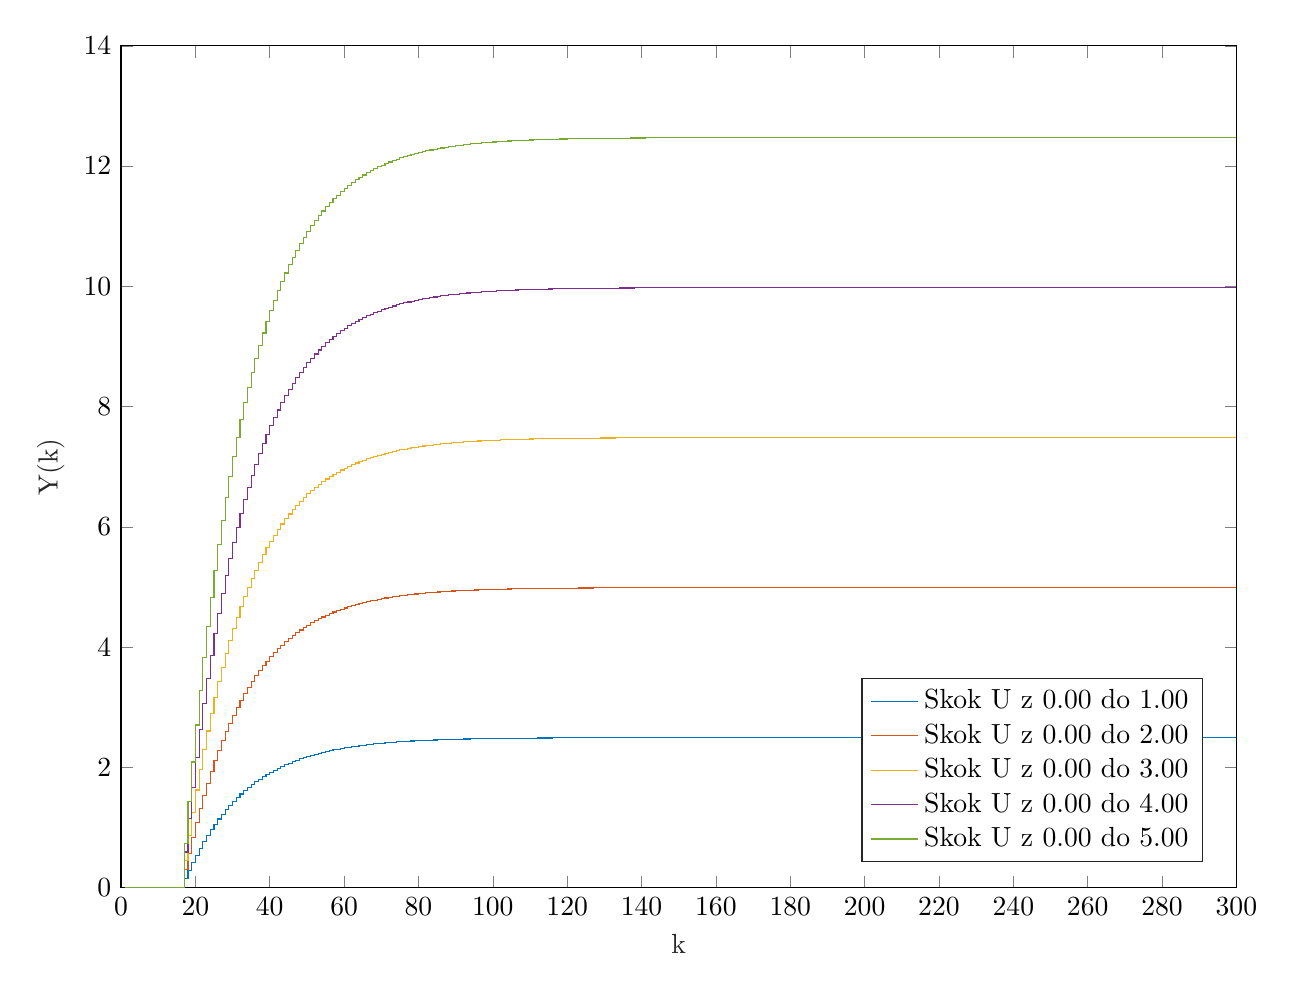
\begin{tikzpicture}

\begin{axis}[%
width=5.577in,
height=4.209in,
at={(0.768in,0.433in)},
scale only axis,
xmin=0,
xmax=300,
xlabel style={font=\color{white!15!black}},
xlabel={k},
ymin=0,
ymax=14,
ylabel style={font=\color{white!15!black}},
ylabel={Y(k)},
axis background/.style={fill=white},
legend style={at={(0.97,0.03)}, anchor=south east, legend cell align=left, align=left, draw=white!15!black}
]
\addplot[const plot, color=mycolor1] table[row sep=crcr] {%
1	0\\
2	0\\
3	0\\
4	0\\
5	0\\
6	0\\
7	0\\
8	0\\
9	0\\
10	0\\
11	0\\
12	0\\
13	0\\
14	0\\
15	0\\
16	0\\
17	0.14788\\
18	0.287003368\\
19	0.4178875887248\\
20	0.541019681620169\\
21	0.656857981328252\\
22	0.765833815583596\\
23	0.868353086271741\\
24	0.964797759090307\\
25	1.05552726696406\\
26	1.14087983209031\\
27	1.2211737112286\\
28	1.29670836859919\\
29	1.36776558051679\\
30	1.43461047566053\\
31	1.4974925146662\\
32	1.55664641252315\\
33	1.61229300706489\\
34	1.6646400766589\\
35	1.71388311002751\\
36	1.76020603096696\\
37	1.8037818805757\\
38	1.84477345945558\\
39	1.88333393220961\\
40	1.91960739642823\\
41	1.95372941823058\\
42	1.98582753630976\\
43	2.01602173631893\\
44	2.04442489733007\\
45	2.07114321199739\\
46	2.09627658196347\\
47	2.11991898995759\\
48	2.14215884995146\\
49	2.16307933665916\\
50	2.18275869559299\\
51	2.20127053481677\\
52	2.2186840994719\\
53	2.23506453008862\\
54	2.25047310563613\\
55	2.26496747220972\\
56	2.27860185820011\\
57	2.29142727674155\\
58	2.30349171618796\\
59	2.31484031932293\\
60	2.32551555196791\\
61	2.33555736161404\\
62	2.34500332666624\\
63	2.35388879685375\\
64	2.3622470253288\\
65	2.37010929294415\\
66	2.37750502517179\\
67	2.38446190209753\\
68	2.39100596190081\\
69	2.39716169820485\\
70	2.40295215165975\\
71	2.40839899609941\\
72	2.41352261959357\\
73	2.41834220069678\\
74	2.42287578017859\\
75	2.42714032850259\\
76	2.43115180930567\\
77	2.43492523911456\\
78	2.43847474352232\\
79	2.44181361003448\\
80	2.44495433778203\\
81	2.44790868428693\\
82	2.45068770945463\\
83	2.45330181695808\\
84	2.45576079316756\\
85	2.45807384377197\\
86	2.46024962822822\\
87	2.46229629216758\\
88	2.46422149788002\\
89	2.46603245299044\\
90	2.46773593743402\\
91	2.46933832883159\\
92	2.47084562635968\\
93	2.47226347320473\\
94	2.47359717768524\\
95	2.47485173312098\\
96	2.47603183652342\\
97	2.47714190617744\\
98	2.47818609817987\\
99	2.47916832199701\\
100	2.48009225509899\\
101	2.48096135672601\\
102	2.48177888083776\\
103	2.48254788829452\\
104	2.48327125831562\\
105	2.48395169925794\\
106	2.48459175875496\\
107	2.48519383325411\\
108	2.4857601769884\\
109	2.48629291041548\\
110	2.48679402815619\\
111	2.48726540646188\\
112	2.48770881023874\\
113	2.48812589965527\\
114	2.48851823635772\\
115	2.48888728931666\\
116	2.48923444032666\\
117	2.48956098917959\\
118	2.48986815853095\\
119	2.49015709847745\\
120	2.49042889086289\\
121	2.49068455332858\\
122	2.49092504312342\\
123	2.49115126068779\\
124	2.49136405302485\\
125	2.49156421687177\\
126	2.49175250168271\\
127	2.49192961243486\\
128	2.4920962122679\\
129	2.49225292496687\\
130	2.49240033729765\\
131	2.4925390012039\\
132	2.49266943587359\\
133	2.4927921296829\\
134	2.49290754202472\\
135	2.49301610502877\\
136	2.49311822517946\\
137	2.49321428483788\\
138	2.4933046436734\\
139	2.49338964001034\\
140	2.4934695920947\\
141	2.49354479928574\\
142	2.4936155431768\\
143	2.49368208864968\\
144	2.49374468486638\\
145	2.49380356620202\\
146	2.49385895312237\\
147	2.49391105300933\\
148	2.4939600609374\\
149	2.49400616040409\\
150	2.49404952401695\\
151	2.49409031413988\\
152	2.49412868350103\\
153	2.49416477576464\\
154	2.49419872606899\\
155	2.49423066153234\\
156	2.49426070172891\\
157	2.4942889591366\\
158	2.49431553955811\\
159	2.49434054251712\\
160	2.49436406163089\\
161	2.49438618496083\\
162	2.49440699534216\\
163	2.49442657069415\\
164	2.49444498431178\\
165	2.49446230514023\\
166	2.49447859803301\\
167	2.49449392399478\\
168	2.49450834040979\\
169	2.4945219012567\\
170	2.49453465731073\\
171	2.49454665633373\\
172	2.49455794325308\\
173	2.49456856032983\\
174	2.49457854731699\\
175	2.49458794160836\\
176	2.49459677837853\\
177	2.4946050907146\\
178	2.49461290974005\\
179	2.49462026473128\\
180	2.49462718322725\\
181	2.49463369113254\\
182	2.4946398128144\\
183	2.49464557119396\\
184	2.49465098783205\\
185	2.49465608300993\\
186	2.49466087580524\\
187	2.49466538416342\\
188	2.4946696249649\\
189	2.49467361408832\\
190	2.49467736646996\\
191	2.49468089615971\\
192	2.49468421637361\\
193	2.49468733954338\\
194	2.49469027736297\\
195	2.49469304083232\\
196	2.49469564029856\\
197	2.49469808549475\\
198	2.49470038557633\\
199	2.49470254915539\\
200	2.49470458433291\\
201	2.49470649872912\\
202	2.49470829951201\\
203	2.49470999342416\\
204	2.49471158680801\\
205	2.4947130856296\\
206	2.4947144955009\\
207	2.49471582170082\\
208	2.49471706919499\\
209	2.49471824265435\\
210	2.49471934647263\\
211	2.4947203847828\\
212	2.49472136147257\\
213	2.49472228019891\\
214	2.49472314440176\\
215	2.49472395731691\\
216	2.49472472198814\\
217	2.49472544127856\\
218	2.49472611788139\\
219	2.49472675432998\\
220	2.49472735300737\\
221	2.49472791615517\\
222	2.49472844588193\\
223	2.4947289441711\\
224	2.49472941288838\\
225	2.49472985378879\\
226	2.49473026852315\\
227	2.49473065864435\\
228	2.4947310256131\\
229	2.49473137080342\\
230	2.49473169550779\\
231	2.49473200094199\\
232	2.49473228824964\\
233	2.4947325585065\\
234	2.49473281272447\\
235	2.49473305185541\\
236	2.49473327679469\\
237	2.49473348838454\\
238	2.4947336874172\\
239	2.49473387463791\\
240	2.49473405074766\\
241	2.49473421640586\\
242	2.49473437223277\\
243	2.49473451881185\\
244	2.49473465669193\\
245	2.49473478638926\\
246	2.49473490838947\\
247	2.49473502314935\\
248	2.4947351310986\\
249	2.49473523264141\\
250	2.49473532815797\\
251	2.49473541800593\\
252	2.49473550252169\\
253	2.49473558202172\\
254	2.49473565680367\\
255	2.49473572714755\\
256	2.49473579331675\\
257	2.49473585555901\\
258	2.49473591410739\\
259	2.49473596918112\\
260	2.49473602098639\\
261	2.49473606971718\\
262	2.49473611555596\\
263	2.49473615867435\\
264	2.4947361992338\\
265	2.49473623738617\\
266	2.49473627327433\\
267	2.49473630703263\\
268	2.49473633878749\\
269	2.4947363686578\\
270	2.4947363967554\\
271	2.49473642318549\\
272	2.49473644804705\\
273	2.49473647143315\\
274	2.49473649343136\\
275	2.49473651412405\\
276	2.49473653358869\\
277	2.49473655189816\\
278	2.49473656912103\\
279	2.49473658532178\\
280	2.49473660056106\\
281	2.49473661489594\\
282	2.49473662838009\\
283	2.49473664106399\\
284	2.49473665299515\\
285	2.49473666421824\\
286	2.49473667477526\\
287	2.49473668470577\\
288	2.49473669404693\\
289	2.49473670283372\\
290	2.49473671109904\\
291	2.49473671887384\\
292	2.49473672618723\\
293	2.4947367330666\\
294	2.49473673953769\\
295	2.49473674562475\\
296	2.49473675135056\\
297	2.49473675673656\\
298	2.49473676180292\\
299	2.49473676656861\\
300	2.49473677105147\\
};
\addlegendentry{Skok U z 0.00 do 1.00}

\addplot[const plot, color=mycolor2] table[row sep=crcr] {%
1	0\\
2	0\\
3	0\\
4	0\\
5	0\\
6	0\\
7	0\\
8	0\\
9	0\\
10	0\\
11	0\\
12	0\\
13	0\\
14	0\\
15	0\\
16	0\\
17	0.29576\\
18	0.574006736\\
19	0.8357751774496\\
20	1.08203936324034\\
21	1.3137159626565\\
22	1.53166763116719\\
23	1.73670617254348\\
24	1.92959551818061\\
25	2.11105453392813\\
26	2.28175966418062\\
27	2.44234742245721\\
28	2.59341673719839\\
29	2.73553116103359\\
30	2.86922095132107\\
31	2.9949850293324\\
32	3.1132928250463\\
33	3.22458601412978\\
34	3.32928015331779\\
35	3.42776622005501\\
36	3.52041206193391\\
37	3.6075637611514\\
38	3.68954691891116\\
39	3.76666786441923\\
40	3.83921479285646\\
41	3.90745883646116\\
42	3.97165507261952\\
43	4.03204347263787\\
44	4.08884979466015\\
45	4.14228642399477\\
46	4.19255316392695\\
47	4.23983797991519\\
48	4.28431769990292\\
49	4.32615867331833\\
50	4.36551739118597\\
51	4.40254106963354\\
52	4.43736819894381\\
53	4.47012906017723\\
54	4.50094621127227\\
55	4.52993494441944\\
56	4.55720371640022\\
57	4.58285455348311\\
58	4.60698343237593\\
59	4.62968063864585\\
60	4.65103110393581\\
61	4.67111472322808\\
62	4.69000665333247\\
63	4.70777759370751\\
64	4.7244940506576\\
65	4.74021858588829\\
66	4.75501005034357\\
67	4.76892380419506\\
68	4.78201192380161\\
69	4.79432339640971\\
70	4.80590430331949\\
71	4.81679799219881\\
72	4.82704523918714\\
73	4.83668440139355\\
74	4.84575156035719\\
75	4.85428065700519\\
76	4.86230361861134\\
77	4.86985047822912\\
78	4.87694948704464\\
79	4.88362722006896\\
80	4.88990867556407\\
81	4.89581736857385\\
82	4.90137541890926\\
83	4.90660363391616\\
84	4.91152158633513\\
85	4.91614768754394\\
86	4.92049925645644\\
87	4.92459258433517\\
88	4.92844299576005\\
89	4.93206490598087\\
90	4.93547187486805\\
91	4.93867665766318\\
92	4.94169125271936\\
93	4.94452694640945\\
94	4.94719435537047\\
95	4.94970346624195\\
96	4.95206367304685\\
97	4.95428381235487\\
98	4.95637219635974\\
99	4.95833664399401\\
100	4.96018451019798\\
101	4.96192271345203\\
102	4.96355776167551\\
103	4.96509577658904\\
104	4.96654251663124\\
105	4.96790339851589\\
106	4.96918351750991\\
107	4.97038766650823\\
108	4.97152035397679\\
109	4.97258582083097\\
110	4.97358805631239\\
111	4.97453081292376\\
112	4.97541762047747\\
113	4.97625179931054\\
114	4.97703647271543\\
115	4.97777457863332\\
116	4.97846888065332\\
117	4.97912197835918\\
118	4.97973631706191\\
119	4.9803141969549\\
120	4.98085778172577\\
121	4.98136910665717\\
122	4.98185008624684\\
123	4.98230252137558\\
124	4.98272810604971\\
125	4.98312843374354\\
126	4.98350500336543\\
127	4.98385922486972\\
128	4.9841924245358\\
129	4.98450584993373\\
130	4.98480067459529\\
131	4.9850780024078\\
132	4.98533887174719\\
133	4.98558425936579\\
134	4.98581508404945\\
135	4.98603221005754\\
136	4.98623645035892\\
137	4.98642856967576\\
138	4.9866092873468\\
139	4.98677928002068\\
140	4.98693918418941\\
141	4.98708959857148\\
142	4.9872310863536\\
143	4.98736417729936\\
144	4.98748936973277\\
145	4.98760713240405\\
146	4.98771790624475\\
147	4.98782210601866\\
148	4.9879201218748\\
149	4.98801232080818\\
150	4.9880990480339\\
151	4.98818062827976\\
152	4.98825736700205\\
153	4.98832955152928\\
154	4.98839745213798\\
155	4.98846132306468\\
156	4.98852140345782\\
157	4.9885779182732\\
158	4.98863107911623\\
159	4.98868108503424\\
160	4.98872812326179\\
161	4.98877236992165\\
162	4.98881399068432\\
163	4.9888531413883\\
164	4.98888996862355\\
165	4.98892461028046\\
166	4.98895719606602\\
167	4.98898784798957\\
168	4.98901668081958\\
169	4.9890438025134\\
170	4.98906931462145\\
171	4.98909331266746\\
172	4.98911588650616\\
173	4.98913712065966\\
174	4.98915709463399\\
175	4.98917588321673\\
176	4.98919355675707\\
177	4.9892101814292\\
178	4.9892258194801\\
179	4.98924052946257\\
180	4.98925436645449\\
181	4.98926738226508\\
182	4.98927962562881\\
183	4.98929114238793\\
184	4.9893019756641\\
185	4.98931216601986\\
186	4.98932175161048\\
187	4.98933076832683\\
188	4.98933924992979\\
189	4.98934722817663\\
190	4.98935473293993\\
191	4.98936179231942\\
192	4.98936843274722\\
193	4.98937467908677\\
194	4.98938055472595\\
195	4.98938608166465\\
196	4.98939128059713\\
197	4.98939617098951\\
198	4.98940077115266\\
199	4.98940509831077\\
200	4.98940916866582\\
201	4.98941299745824\\
202	4.98941659902401\\
203	4.98941998684831\\
204	4.98942317361602\\
205	4.9894261712592\\
206	4.98942899100179\\
207	4.98943164340163\\
208	4.98943413838998\\
209	4.9894364853087\\
210	4.98943869294526\\
211	4.98944076956561\\
212	4.98944272294514\\
213	4.98944456039781\\
214	4.98944628880351\\
215	4.98944791463383\\
216	4.98944944397628\\
217	4.98945088255713\\
218	4.98945223576277\\
219	4.98945350865996\\
220	4.98945470601475\\
221	4.98945583231034\\
222	4.98945689176386\\
223	4.98945788834219\\
224	4.98945882577676\\
225	4.98945970757757\\
226	4.98946053704631\\
227	4.98946131728871\\
228	4.98946205122621\\
229	4.98946274160684\\
230	4.98946339101559\\
231	4.98946400188398\\
232	4.98946457649928\\
233	4.98946511701299\\
234	4.98946562544893\\
235	4.98946610371081\\
236	4.98946655358937\\
237	4.98946697676907\\
238	4.9894673748344\\
239	4.98946774927581\\
240	4.98946810149532\\
241	4.98946843281172\\
242	4.98946874446554\\
243	4.9894690376237\\
244	4.98946931338386\\
245	4.98946957277852\\
246	4.98946981677894\\
247	4.98947004629871\\
248	4.98947026219721\\
249	4.98947046528282\\
250	4.98947065631594\\
251	4.98947083601185\\
252	4.98947100504339\\
253	4.98947116404344\\
254	4.98947131360734\\
255	4.9894714542951\\
256	4.98947158663349\\
257	4.98947171111802\\
258	4.98947182821479\\
259	4.98947193836223\\
260	4.98947204197277\\
261	4.98947213943436\\
262	4.98947223111191\\
263	4.98947231734869\\
264	4.98947239846759\\
265	4.98947247477234\\
266	4.98947254654865\\
267	4.98947261406526\\
268	4.98947267757498\\
269	4.98947273731559\\
270	4.98947279351079\\
271	4.98947284637099\\
272	4.9894728960941\\
273	4.9894729428663\\
274	4.98947298686272\\
275	4.98947302824809\\
276	4.98947306717738\\
277	4.98947310379633\\
278	4.98947313824206\\
279	4.98947317064355\\
280	4.98947320112212\\
281	4.98947322979187\\
282	4.98947325676017\\
283	4.98947328212799\\
284	4.9894733059903\\
285	4.98947332843647\\
286	4.98947334955053\\
287	4.98947336941153\\
288	4.98947338809385\\
289	4.98947340566743\\
290	4.98947342219807\\
291	4.98947343774768\\
292	4.98947345237446\\
293	4.98947346613319\\
294	4.98947347907538\\
295	4.9894734912495\\
296	4.98947350270112\\
297	4.98947351347313\\
298	4.98947352360585\\
299	4.98947353313722\\
300	4.98947354210294\\
};
\addlegendentry{Skok U z 0.00 do 2.00}

\addplot[const plot, color=mycolor3] table[row sep=crcr] {%
1	0\\
2	0\\
3	0\\
4	0\\
5	0\\
6	0\\
7	0\\
8	0\\
9	0\\
10	0\\
11	0\\
12	0\\
13	0\\
14	0\\
15	0\\
16	0\\
17	0.44364\\
18	0.861010104\\
19	1.2536627661744\\
20	1.62305904486051\\
21	1.97057394398476\\
22	2.29750144675079\\
23	2.60505925881522\\
24	2.89439327727092\\
25	3.16658180089219\\
26	3.42263949627092\\
27	3.6635211336858\\
28	3.89012510579757\\
29	4.10329674155037\\
30	4.30383142698159\\
31	4.49247754399859\\
32	4.66993923756944\\
33	4.83687902119467\\
34	4.99392022997669\\
35	5.14164933008253\\
36	5.28061809290088\\
37	5.41134564172712\\
38	5.53432037836675\\
39	5.65000179662886\\
40	5.75882218928471\\
41	5.86118825469177\\
42	5.95748260892931\\
43	6.04806520895684\\
44	6.13327469199027\\
45	6.2134296359922\\
46	6.28882974589047\\
47	6.35975696987283\\
48	6.42647654985444\\
49	6.48923800997755\\
50	6.54827608677902\\
51	6.60381160445037\\
52	6.65605229841577\\
53	6.70519359026591\\
54	6.75141931690847\\
55	6.79490241662923\\
56	6.83580557460041\\
57	6.87428183022474\\
58	6.91047514856397\\
59	6.94452095796886\\
60	6.97654665590381\\
61	7.00667208484221\\
62	7.03500997999881\\
63	7.06166639056137\\
64	7.08674107598651\\
65	7.11032787883256\\
66	7.13251507551547\\
67	7.1533857062927\\
68	7.17301788570254\\
69	7.19148509461468\\
70	7.20885645497936\\
71	7.22519698829834\\
72	7.24056785878084\\
73	7.25502660209046\\
74	7.26862734053591\\
75	7.28142098550791\\
76	7.29345542791715\\
77	7.30477571734382\\
78	7.31542423056711\\
79	7.32544083010359\\
80	7.33486301334624\\
81	7.34372605286092\\
82	7.35206312836403\\
83	7.35990545087438\\
84	7.36728237950284\\
85	7.37422153131606\\
86	7.38074888468481\\
87	7.3868888765029\\
88	7.39266449364021\\
89	7.39809735897145\\
90	7.40320781230221\\
91	7.40801498649491\\
92	7.41253687907917\\
93	7.41679041961431\\
94	7.42079153305584\\
95	7.42455519936306\\
96	7.4280955095704\\
97	7.43142571853244\\
98	7.43455829453974\\
99	7.43750496599115\\
100	7.4402767652971\\
101	7.44288407017817\\
102	7.4453366425134\\
103	7.44764366488369\\
104	7.44981377494699\\
105	7.45185509777397\\
106	7.45377527626501\\
107	7.45558149976249\\
108	7.45728053096533\\
109	7.45887873124659\\
110	7.46038208446872\\
111	7.46179621938579\\
112	7.46312643071635\\
113	7.46437769896595\\
114	7.46555470907329\\
115	7.46666186795012\\
116	7.46770332098012\\
117	7.46868296753891\\
118	7.469604475593\\
119	7.47047129543249\\
120	7.4712866725888\\
121	7.47205365998589\\
122	7.47277512937041\\
123	7.47345378206351\\
124	7.4740921590747\\
125	7.47469265061545\\
126	7.47525750504827\\
127	7.47578883730472\\
128	7.47628863680383\\
129	7.47675877490073\\
130	7.47720101189306\\
131	7.47761700361183\\
132	7.4780083076209\\
133	7.47837638904881\\
134	7.47872262607429\\
135	7.47904831508643\\
136	7.47935467553849\\
137	7.47964285451375\\
138	7.47991393102032\\
139	7.48016892003114\\
140	7.48040877628423\\
141	7.48063439785733\\
142	7.48084662953051\\
143	7.48104626594916\\
144	7.48123405459927\\
145	7.48141069860619\\
146	7.48157685936724\\
147	7.48173315902812\\
148	7.48188018281232\\
149	7.48201848121238\\
150	7.48214857205097\\
151	7.48227094241976\\
152	7.4823860505032\\
153	7.48249432729405\\
154	7.4825961782071\\
155	7.48269198459715\\
156	7.48278210518687\\
157	7.48286687740994\\
158	7.48294661867448\\
159	7.4830216275515\\
160	7.48309218489282\\
161	7.48315855488262\\
162	7.48322098602663\\
163	7.48327971208259\\
164	7.48333495293548\\
165	7.48338691542084\\
166	7.48343579409918\\
167	7.48348177198451\\
168	7.48352502122954\\
169	7.48356570377027\\
170	7.48360397193234\\
171	7.48363996900136\\
172	7.4836738297594\\
173	7.48370568098966\\
174	7.48373564195114\\
175	7.48376382482525\\
176	7.48379033513576\\
177	7.48381527214396\\
178	7.4838387292203\\
179	7.483860794194\\
180	7.48388154968189\\
181	7.48390107339777\\
182	7.48391943844337\\
183	7.48393671358205\\
184	7.48395296349632\\
185	7.48396824902996\\
186	7.48398262741588\\
187	7.48399615249041\\
188	7.48400887489484\\
189	7.4840208422651\\
190	7.48403209941004\\
191	7.48404268847928\\
192	7.48405264912097\\
193	7.48406201863029\\
194	7.48407083208906\\
195	7.48407912249711\\
196	7.48408692089582\\
197	7.48409425648439\\
198	7.48410115672912\\
199	7.48410764746628\\
200	7.48411375299885\\
201	7.48411949618748\\
202	7.48412489853614\\
203	7.48412998027259\\
204	7.48413476042415\\
205	7.48413925688892\\
206	7.48414348650281\\
207	7.48414746510257\\
208	7.48415120758508\\
209	7.48415472796316\\
210	7.484158039418\\
211	7.48416115434852\\
212	7.48416408441782\\
213	7.48416684059683\\
214	7.48416943320537\\
215	7.48417187195085\\
216	7.48417416596453\\
217	7.48417632383579\\
218	7.48417835364426\\
219	7.48418026299005\\
220	7.48418205902223\\
221	7.48418374846562\\
222	7.48418533764591\\
223	7.4841868325134\\
224	7.48418823866526\\
225	7.48418956136648\\
226	7.48419080556958\\
227	7.48419197593319\\
228	7.48419307683943\\
229	7.48419411241039\\
230	7.48419508652351\\
231	7.48419600282611\\
232	7.48419686474906\\
233	7.48419767551962\\
234	7.48419843817353\\
235	7.48419915556635\\
236	7.48419983038419\\
237	7.48420046515374\\
238	7.48420106225173\\
239	7.48420162391385\\
240	7.48420215224311\\
241	7.48420264921771\\
242	7.48420311669845\\
243	7.48420355643569\\
244	7.48420397007592\\
245	7.48420435916792\\
246	7.48420472516855\\
247	7.4842050694482\\
248	7.48420539329596\\
249	7.48420569792437\\
250	7.48420598447406\\
251	7.48420625401794\\
252	7.48420650756524\\
253	7.48420674606532\\
254	7.48420697041117\\
255	7.48420718144281\\
256	7.4842073799504\\
257	7.48420756667718\\
258	7.48420774232233\\
259	7.4842079075435\\
260	7.48420806295931\\
261	7.48420820915169\\
262	7.48420834666802\\
263	7.48420847602319\\
264	7.48420859770154\\
265	7.48420871215867\\
266	7.48420881982313\\
267	7.48420892109805\\
268	7.48420901636262\\
269	7.48420910597354\\
270	7.48420919026634\\
271	7.48420926955663\\
272	7.48420934414129\\
273	7.48420941429959\\
274	7.48420948029422\\
275	7.48420954237228\\
276	7.4842096007662\\
277	7.48420965569462\\
278	7.48420970736322\\
279	7.48420975596545\\
280	7.4842098016833\\
281	7.48420984468793\\
282	7.48420988514038\\
283	7.4842099231921\\
284	7.48420995898558\\
285	7.48420999265482\\
286	7.48421002432591\\
287	7.48421005411741\\
288	7.48421008214089\\
289	7.48421010850126\\
290	7.48421013329722\\
291	7.48421015662163\\
292	7.4842101785618\\
293	7.4842101991999\\
294	7.48421021861319\\
295	7.48421023687436\\
296	7.48421025405179\\
297	7.4842102702098\\
298	7.48421028540888\\
299	7.48421029970594\\
300	7.48421031315451\\
};
\addlegendentry{Skok U z 0.00 do 3.00}

\addplot[const plot, color=mycolor4] table[row sep=crcr] {%
1	0\\
2	0\\
3	0\\
4	0\\
5	0\\
6	0\\
7	0\\
8	0\\
9	0\\
10	0\\
11	0\\
12	0\\
13	0\\
14	0\\
15	0\\
16	0\\
17	0.59152\\
18	1.148013472\\
19	1.6715503548992\\
20	2.16407872648068\\
21	2.62743192531301\\
22	3.06333526233438\\
23	3.47341234508696\\
24	3.85919103636123\\
25	4.22210906785626\\
26	4.56351932836123\\
27	4.88469484491441\\
28	5.18683347439677\\
29	5.47106232206718\\
30	5.73844190264213\\
31	5.9899700586648\\
32	6.2265856500926\\
33	6.44917202825956\\
34	6.65856030663558\\
35	6.85553244011003\\
36	7.04082412386783\\
37	7.21512752230281\\
38	7.37909383782231\\
39	7.53333572883846\\
40	7.67842958571292\\
41	7.81491767292232\\
42	7.94331014523904\\
43	8.06408694527573\\
44	8.1776995893203\\
45	8.28457284798954\\
46	8.3851063278539\\
47	8.47967595983037\\
48	8.56863539980585\\
49	8.65231734663665\\
50	8.73103478237195\\
51	8.80508213926708\\
52	8.87473639788762\\
53	8.94025812035446\\
54	9.00189242254454\\
55	9.05986988883888\\
56	9.11440743280045\\
57	9.16570910696622\\
58	9.21396686475185\\
59	9.2593612772917\\
60	9.30206220787162\\
61	9.34222944645615\\
62	9.38001330666495\\
63	9.41555518741502\\
64	9.44898810131521\\
65	9.48043717177659\\
66	9.51002010068714\\
67	9.53784760839011\\
68	9.56402384760322\\
69	9.58864679281941\\
70	9.61180860663898\\
71	9.63359598439762\\
72	9.65409047837429\\
73	9.6733688027871\\
74	9.69150312071437\\
75	9.70856131401037\\
76	9.72460723722269\\
77	9.73970095645824\\
78	9.75389897408929\\
79	9.76725444013793\\
80	9.77981735112814\\
81	9.7916347371477\\
82	9.80275083781851\\
83	9.81320726783231\\
84	9.82304317267026\\
85	9.83229537508789\\
86	9.84099851291288\\
87	9.84918516867034\\
88	9.85688599152009\\
89	9.86412981196175\\
90	9.87094374973609\\
91	9.87735331532637\\
92	9.88338250543872\\
93	9.8890538928189\\
94	9.89438871074095\\
95	9.89940693248391\\
96	9.9041273460937\\
97	9.90856762470975\\
98	9.91274439271948\\
99	9.91667328798803\\
100	9.92036902039596\\
101	9.92384542690405\\
102	9.92711552335103\\
103	9.93019155317807\\
104	9.93308503326248\\
105	9.93580679703178\\
106	9.93836703501983\\
107	9.94077533301646\\
108	9.94304070795359\\
109	9.94517164166193\\
110	9.94717611262477\\
111	9.94906162584753\\
112	9.95083524095495\\
113	9.95250359862107\\
114	9.95407294543087\\
115	9.95554915726663\\
116	9.95693776130663\\
117	9.95824395671835\\
118	9.95947263412381\\
119	9.9606283939098\\
120	9.96171556345154\\
121	9.96273821331433\\
122	9.96370017249369\\
123	9.96460504275116\\
124	9.96545621209942\\
125	9.96625686748709\\
126	9.96701000673085\\
127	9.96771844973944\\
128	9.9683848490716\\
129	9.96901169986746\\
130	9.96960134919058\\
131	9.9701560048156\\
132	9.97067774349438\\
133	9.97116851873158\\
134	9.97163016809889\\
135	9.97206442011508\\
136	9.97247290071784\\
137	9.97285713935151\\
138	9.9732185746936\\
139	9.97355856004137\\
140	9.97387836837882\\
141	9.97417919714295\\
142	9.97446217270719\\
143	9.97472835459872\\
144	9.97497873946554\\
145	9.9752142648081\\
146	9.9754358124895\\
147	9.97564421203733\\
148	9.97584024374961\\
149	9.97602464161635\\
150	9.9761980960678\\
151	9.97636125655952\\
152	9.9765147340041\\
153	9.97665910305856\\
154	9.97679490427596\\
155	9.97692264612935\\
156	9.97704280691564\\
157	9.9771558365464\\
158	9.97726215823245\\
159	9.97736217006848\\
160	9.97745624652357\\
161	9.9775447398433\\
162	9.97762798136865\\
163	9.97770628277659\\
164	9.97777993724711\\
165	9.97784922056091\\
166	9.97791439213204\\
167	9.97797569597914\\
168	9.97803336163917\\
169	9.97808760502681\\
170	9.9781386292429\\
171	9.97818662533493\\
172	9.97823177301232\\
173	9.97827424131932\\
174	9.97831418926797\\
175	9.97835176643345\\
176	9.97838711351413\\
177	9.9784203628584\\
178	9.97845163896019\\
179	9.97848105892513\\
180	9.97850873290899\\
181	9.97853476453016\\
182	9.97855925125761\\
183	9.97858228477586\\
184	9.97860395132821\\
185	9.97862433203973\\
186	9.97864350322096\\
187	9.97866153665367\\
188	9.97867849985959\\
189	9.97869445635327\\
190	9.97870946587986\\
191	9.97872358463884\\
192	9.97873686549444\\
193	9.97874935817353\\
194	9.9787611094519\\
195	9.97877216332929\\
196	9.97878256119425\\
197	9.97879234197901\\
198	9.97880154230532\\
199	9.97881019662154\\
200	9.97881833733163\\
201	9.97882599491648\\
202	9.97883319804802\\
203	9.97883997369663\\
204	9.97884634723204\\
205	9.9788523425184\\
206	9.97885798200359\\
207	9.97886328680326\\
208	9.97886827677995\\
209	9.9788729706174\\
210	9.97887738589051\\
211	9.97888153913121\\
212	9.97888544589028\\
213	9.97888912079563\\
214	9.97889257760703\\
215	9.97889582926766\\
216	9.97889888795257\\
217	9.97890176511425\\
218	9.97890447152554\\
219	9.97890701731992\\
220	9.9789094120295\\
221	9.97891166462068\\
222	9.97891378352773\\
223	9.97891577668438\\
224	9.97891765155352\\
225	9.97891941515514\\
226	9.97892107409261\\
227	9.97892263457742\\
228	9.97892410245241\\
229	9.97892548321369\\
230	9.97892678203117\\
231	9.97892800376797\\
232	9.97892915299857\\
233	9.97893023402599\\
234	9.97893125089786\\
235	9.97893220742163\\
236	9.97893310717875\\
237	9.97893395353814\\
238	9.97893474966879\\
239	9.97893549855162\\
240	9.97893620299063\\
241	9.97893686562343\\
242	9.97893748893108\\
243	9.9789380752474\\
244	9.97893862676772\\
245	9.97893914555705\\
246	9.97893963355788\\
247	9.97894009259742\\
248	9.97894052439442\\
249	9.97894093056563\\
250	9.97894131263188\\
251	9.97894167202371\\
252	9.97894201008678\\
253	9.97894232808688\\
254	9.97894262721468\\
255	9.97894290859021\\
256	9.97894317326699\\
257	9.97894342223604\\
258	9.97894365642957\\
259	9.97894387672446\\
260	9.97894408394555\\
261	9.97894427886872\\
262	9.97894446222382\\
263	9.97894463469738\\
264	9.97894479693518\\
265	9.97894494954469\\
266	9.9789450930973\\
267	9.97894522813053\\
268	9.97894535514996\\
269	9.97894547463119\\
270	9.97894558702159\\
271	9.97894569274198\\
272	9.9789457921882\\
273	9.9789458857326\\
274	9.97894597372544\\
275	9.97894605649619\\
276	9.97894613435475\\
277	9.97894620759265\\
278	9.97894627648412\\
279	9.9789463412871\\
280	9.97894640224423\\
281	9.97894645958375\\
282	9.97894651352034\\
283	9.97894656425597\\
284	9.97894661198061\\
285	9.97894665687294\\
286	9.97894669910106\\
287	9.97894673882307\\
288	9.9789467761877\\
289	9.97894681133486\\
290	9.97894684439615\\
291	9.97894687549535\\
292	9.97894690474892\\
293	9.97894693226638\\
294	9.97894695815077\\
295	9.978946982499\\
296	9.97894700540225\\
297	9.97894702694626\\
298	9.9789470472117\\
299	9.97894706627445\\
300	9.97894708420588\\
};
\addlegendentry{Skok U z 0.00 do 4.00}

\addplot[const plot, color=mycolor5] table[row sep=crcr] {%
1	0\\
2	0\\
3	0\\
4	0\\
5	0\\
6	0\\
7	0\\
8	0\\
9	0\\
10	0\\
11	0\\
12	0\\
13	0\\
14	0\\
15	0\\
16	0\\
17	0.7394\\
18	1.43501684\\
19	2.089437943624\\
20	2.70509840810085\\
21	3.28428990664126\\
22	3.82916907791798\\
23	4.3417654313587\\
24	4.82398879545153\\
25	5.27763633482032\\
26	5.70439916045154\\
27	6.10586855614302\\
28	6.48354184299597\\
29	6.83882790258398\\
30	7.17305237830268\\
31	7.48746257333101\\
32	7.78323206261577\\
33	8.06146503532447\\
34	8.32320038329451\\
35	8.56941555013757\\
36	8.80103015483482\\
37	9.01890940287855\\
38	9.22386729727793\\
39	9.41666966104811\\
40	9.59803698214119\\
41	9.76864709115294\\
42	9.92913768154884\\
43	10.0801086815947\\
44	10.2221244866504\\
45	10.355716059987\\
46	10.4813829098174\\
47	10.599594949788\\
48	10.7107942497574\\
49	10.8153966832959\\
50	10.913793477965\\
51	11.0063526740839\\
52	11.0934204973596\\
53	11.1753226504432\\
54	11.2523655281807\\
55	11.3248373610487\\
56	11.3930092910006\\
57	11.4571363837079\\
58	11.5174585809399\\
59	11.5742015966147\\
60	11.6275777598396\\
61	11.6777868080703\\
62	11.7250166333313\\
63	11.7694439842689\\
64	11.8112351266441\\
65	11.8505464647209\\
66	11.8875251258591\\
67	11.9223095104878\\
68	11.9550298095042\\
69	11.9858084910244\\
70	12.0147607582989\\
71	12.0419949804972\\
72	12.067613097968\\
73	12.0917110034841\\
74	12.1143789008931\\
75	12.1357016425132\\
76	12.1557590465285\\
77	12.174626195573\\
78	12.1923737176118\\
79	12.2090680501726\\
80	12.2247716889104\\
81	12.2395434214348\\
82	12.2534385472733\\
83	12.2665090847906\\
84	12.278803965838\\
85	12.29036921886\\
86	12.3012481411413\\
87	12.3114814608381\\
88	12.3211074894003\\
89	12.3301622649523\\
90	12.3386796871703\\
91	12.3466916441581\\
92	12.3542281317985\\
93	12.3613173660238\\
94	12.3679858884263\\
95	12.374258665605\\
96	12.3801591826172\\
97	12.3857095308873\\
98	12.3909304908995\\
99	12.3958416099852\\
100	12.4004612754951\\
101	12.4048067836302\\
102	12.4088944041889\\
103	12.4127394414727\\
104	12.4163562915782\\
105	12.4197584962899\\
106	12.4229587937749\\
107	12.4259691662707\\
108	12.4288008849421\\
109	12.4314645520775\\
110	12.4339701407811\\
111	12.4363270323096\\
112	12.4385440511938\\
113	12.4406294982765\\
114	12.4425911817887\\
115	12.4444364465834\\
116	12.4461722016334\\
117	12.4478049458981\\
118	12.4493407926549\\
119	12.4507854923874\\
120	12.4521444543146\\
121	12.4534227666431\\
122	12.4546252156173\\
123	12.4557563034391\\
124	12.4568202651244\\
125	12.457821084359\\
126	12.4587625084137\\
127	12.4596480621744\\
128	12.4604810613396\\
129	12.4612646248344\\
130	12.4620016864883\\
131	12.4626950060196\\
132	12.4633471793681\\
133	12.4639606484146\\
134	12.4645377101237\\
135	12.465080525144\\
136	12.4655911258974\\
137	12.4660714241895\\
138	12.4665232183671\\
139	12.4669482000518\\
140	12.4673479604736\\
141	12.4677239964288\\
142	12.4680777158841\\
143	12.4684104432485\\
144	12.468723424332\\
145	12.4690178310102\\
146	12.469294765612\\
147	12.4695552650467\\
148	12.4698003046871\\
149	12.4700308020205\\
150	12.4702476200848\\
151	12.4704515706995\\
152	12.4706434175052\\
153	12.4708238788233\\
154	12.470993630345\\
155	12.4711533076618\\
156	12.4713035086446\\
157	12.4714447956831\\
158	12.4715776977907\\
159	12.4717027125857\\
160	12.4718203081546\\
161	12.4719309248042\\
162	12.4720349767109\\
163	12.4721328534708\\
164	12.472224921559\\
165	12.4723115257012\\
166	12.4723929901651\\
167	12.472469619974\\
168	12.472541702049\\
169	12.4726095062836\\
170	12.4726732865537\\
171	12.4727332816687\\
172	12.4727897162655\\
173	12.4728428016492\\
174	12.472892736585\\
175	12.4729397080419\\
176	12.4729838918927\\
177	12.4730254535731\\
178	12.4730645487003\\
179	12.4731013236565\\
180	12.4731359161363\\
181	12.4731684556628\\
182	12.4731990640721\\
183	12.4732278559699\\
184	12.4732549391604\\
185	12.4732804150498\\
186	12.4733043790263\\
187	12.4733269208172\\
188	12.4733481248246\\
189	12.4733680704417\\
190	12.4733868323499\\
191	12.4734044807987\\
192	12.4734210818682\\
193	12.473436697717\\
194	12.473451386815\\
195	12.4734652041617\\
196	12.4734782014929\\
197	12.4734904274739\\
198	12.4735019278818\\
199	12.473512745777\\
200	12.4735229216646\\
201	12.4735324936457\\
202	12.4735414975601\\
203	12.4735499671209\\
204	12.4735579340401\\
205	12.4735654281481\\
206	12.4735724775046\\
207	12.4735791085042\\
208	12.473585345975\\
209	12.4735912132718\\
210	12.4735967323632\\
211	12.4736019239141\\
212	12.4736068073629\\
213	12.4736114009946\\
214	12.4736157220088\\
215	12.4736197865846\\
216	12.4736236099408\\
217	12.4736272063929\\
218	12.473630589407\\
219	12.47363377165\\
220	12.473636765037\\
221	12.4736395807759\\
222	12.4736422294098\\
223	12.4736447208556\\
224	12.473647064442\\
225	12.473649268944\\
226	12.4736513426159\\
227	12.4736532932219\\
228	12.4736551280656\\
229	12.4736568540172\\
230	12.4736584775391\\
231	12.4736600047101\\
232	12.4736614412483\\
233	12.4736627925326\\
234	12.4736640636225\\
235	12.4736652592772\\
236	12.4736663839736\\
237	12.4736674419228\\
238	12.4736684370861\\
239	12.4736693731897\\
240	12.4736702537385\\
241	12.4736710820295\\
242	12.473671861164\\
243	12.4736725940594\\
244	12.4736732834598\\
245	12.4736739319465\\
246	12.4736745419475\\
247	12.4736751157469\\
248	12.4736756554932\\
249	12.4736761632072\\
250	12.47367664079\\
251	12.4736770900298\\
252	12.4736775126086\\
253	12.4736779101088\\
254	12.4736782840185\\
255	12.4736786357379\\
256	12.4736789665839\\
257	12.4736792777952\\
258	12.4736795705371\\
259	12.4736798459057\\
260	12.4736801049321\\
261	12.473680348586\\
262	12.4736805777799\\
263	12.4736807933719\\
264	12.4736809961691\\
265	12.473681186931\\
266	12.4736813663718\\
267	12.4736815351633\\
268	12.4736816939376\\
269	12.4736818432891\\
270	12.4736819837771\\
271	12.4736821159276\\
272	12.4736822402354\\
273	12.4736823571659\\
274	12.4736824671569\\
275	12.4736825706203\\
276	12.4736826679435\\
277	12.4736827594909\\
278	12.4736828456053\\
279	12.473682926609\\
280	12.4736830028054\\
281	12.4736830744798\\
282	12.4736831419005\\
283	12.4736832053201\\
284	12.4736832649759\\
285	12.4736833210913\\
286	12.4736833738764\\
287	12.4736834235289\\
288	12.4736834702347\\
289	12.4736835141687\\
290	12.4736835554953\\
291	12.4736835943693\\
292	12.4736836309362\\
293	12.4736836653331\\
294	12.4736836976885\\
295	12.4736837281238\\
296	12.4736837567529\\
297	12.4736837836829\\
298	12.4736838090147\\
299	12.4736838328431\\
300	12.4736838552574\\
};
\addlegendentry{Skok U z 0.00 do 5.00}

\end{axis}
\end{tikzpicture}%
\caption{Wykresy odpowiedzi skokowych toru U-Y}
\end{figure}

Jak widać wartość skoku na wyjściu jest proporcjonalna wartości skoku wejścia.

\section{Opowiedzi skokowe toru Z-Y}

\begin{figure}[H]
\centering
% This file was created by matlab2tikz.
%
%The latest updates can be retrieved from
%  http://www.mathworks.com/matlabcentral/fileexchange/22022-matlab2tikz-matlab2tikz
%where you can also make suggestions and rate matlab2tikz.
%
\definecolor{mycolor1}{rgb}{0.00000,0.44700,0.74100}%
\definecolor{mycolor2}{rgb}{0.85000,0.32500,0.09800}%
\definecolor{mycolor3}{rgb}{0.92900,0.69400,0.12500}%
\definecolor{mycolor4}{rgb}{0.49400,0.18400,0.55600}%
\definecolor{mycolor5}{rgb}{0.46600,0.67400,0.18800}%
%
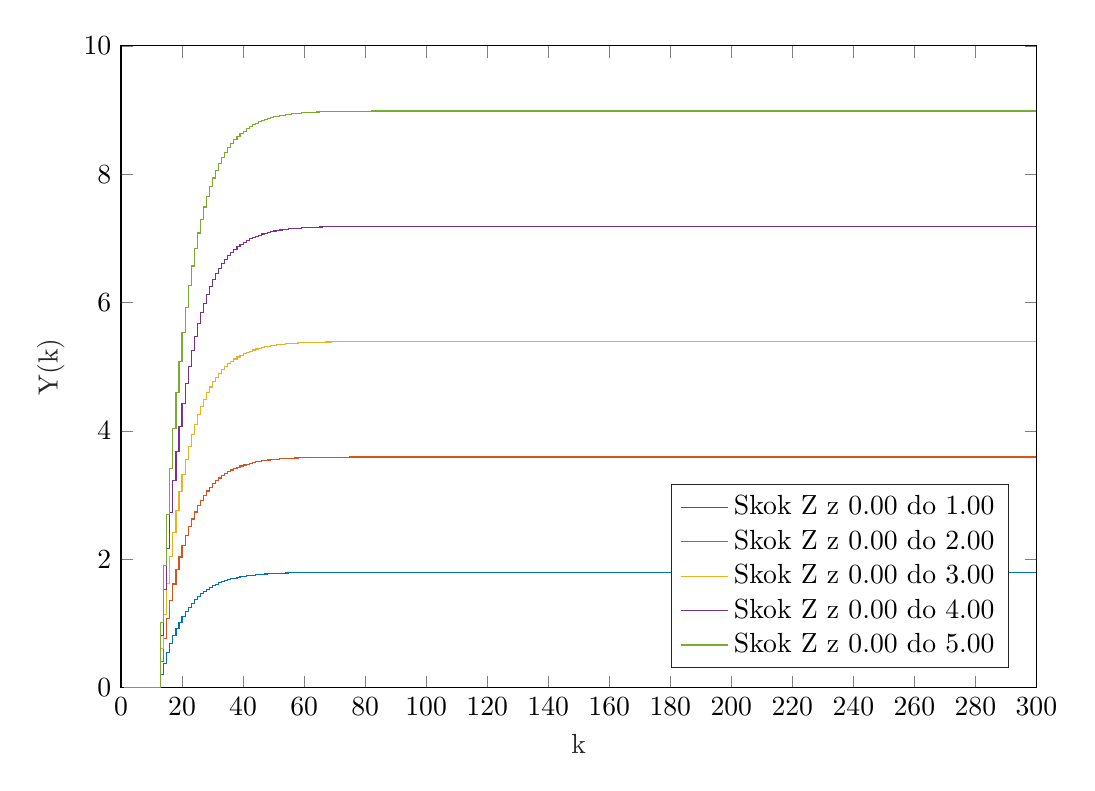
\begin{tikzpicture}

\begin{axis}[%
width=4.577in,
height=3.209in,
at={(0.768in,0.433in)},
scale only axis,
xmin=0,
xmax=300,
xlabel style={font=\color{white!15!black}},
xlabel={k},
ymin=0,
ymax=10,
ylabel style={font=\color{white!15!black}},
ylabel={Y(k)},
axis background/.style={fill=white},
legend style={at={(0.97,0.03)}, anchor=south east, legend cell align=left, align=left, draw=white!15!black}
]
\addplot[const plot, color=mycolor1] table[row sep=crcr] {%
1	0\\
2	0\\
3	0\\
4	0\\
5	0\\
6	0\\
7	0\\
8	0\\
9	0\\
10	0\\
11	0\\
12	0\\
13	0.20202\\
14	0.381363772\\
15	0.5405745884792\\
16	0.681910601930065\\
17	0.807376801662065\\
18	0.918753389257166\\
19	1.01762097400741\\
20	1.10538294469291\\
21	1.18328533412576\\
22	1.25243445742761\\
23	1.31381257352359\\
24	1.36829179137883\\
25	1.41664641767974\\
26	1.45956392062001\\
27	1.49765466487875\\
28	1.53146055549941\\
29	1.56146271294626\\
30	1.58808828791264\\
31	1.61171651228869\\
32	1.63268407189206\\
33	1.6512898769727\\
34	1.66779929798444\\
35	1.68244792655289\\
36	1.69544491485312\\
37	1.70697594064711\\
38	1.71720583993623\\
39	1.7262809444819\\
40	1.73433115727287\\
41	1.74147179531066\\
42	1.7478052257929\\
43	1.75342231885168\\
44	1.75840373740865\\
45	1.7628210824046\\
46	1.76673790961448\\
47	1.77021063244259\\
48	1.77328932347903\\
49	1.77601842616608\\
50	1.77843738665143\\
51	1.78058121477559\\
52	1.78248098213803\\
53	1.7841642642963\\
54	1.78565553336142\\
55	1.78697650655121\\
56	1.78814645563942\\
57	1.78918248168534\\
58	1.79009975893699\\
59	1.7909117513645\\
60	1.791630404893\\
61	1.79226631806014\\
62	1.7928288935179\\
63	1.7933264725271\\
64	1.79376645435222\\
65	1.79415540225022\\
66	1.79449913755705\\
67	1.79480282320733\\
68	1.7950710378724\\
69	1.79530784176955\\
70	1.79551683507687\\
71	1.79570120978355\\
72	1.79586379571225\\
73	1.79600710136771\\
74	1.79613335019233\\
75	1.79624451274432\\
76	1.79634233525612\\
77	1.79642836497965\\
78	1.79650397267911\\
79	1.79657037259177\\
80	1.79662864014108\\
81	1.7966797276547\\
82	1.79672447831156\\
83	1.79676363851692\\
84	1.79679786888231\\
85	1.79682775396694\\
86	1.79685381091999\\
87	1.79687649714742\\
88	1.79689621711284\\
89	1.79691332837016\\
90	1.79692814691417\\
91	1.79694095192608\\
92	1.79695198998197\\
93	1.79696147878477\\
94	1.79696961047339\\
95	1.79697655455666\\
96	1.79698246051441\\
97	1.79698746010321\\
98	1.79699166940006\\
99	1.79699519061374\\
100	1.79699811368989\\
101	1.79700051773321\\
102	1.79700247226746\\
103	1.79700403835162\\
104	1.79700526956837\\
105	1.79700621289954\\
106	1.79700690950111\\
107	1.79700739538939\\
108	1.79700770204824\\
109	1.79700785696642\\
110	1.797007884113\\
111	1.79700780435784\\
112	1.79700763584335\\
113	1.79700739431327\\
114	1.79700709340309\\
115	1.79700674489673\\
116	1.79700635895323\\
117	1.79700594430688\\
118	1.79700550844388\\
119	1.79700505775816\\
120	1.79700459768881\\
121	1.79700413284126\\
122	1.79700366709395\\
123	1.79700320369234\\
124	1.79700274533158\\
125	1.79700229422931\\
126	1.79700185218951\\
127	1.7970014206587\\
128	1.79700100077522\\
129	1.79700059341239\\
130	1.79700019921639\\
131	1.79699981863939\\
132	1.7969994519685\\
133	1.79699909935105\\
134	1.79699876081664\\
135	1.79699843629634\\
136	1.79699812563939\\
137	1.79699782862767\\
138	1.79699754498826\\
139	1.79699727440427\\
140	1.7969970165242\\
141	1.79699677096999\\
142	1.79699653734388\\
143	1.79699631523434\\
144	1.79699610422104\\
145	1.79699590387911\\
146	1.79699571378272\\
147	1.79699553350805\\
148	1.7969953626358\\
149	1.79699520075323\\
150	1.7969950474558\\
151	1.79699490234855\\
152	1.79699476504709\\
153	1.79699463517849\\
154	1.7969945123818\\
155	1.79699439630853\\
156	1.79699428662288\\
157	1.7969941830019\\
158	1.79699408513551\\
159	1.79699399272646\\
160	1.79699390549016\\
161	1.79699382315454\\
162	1.79699374545974\\
163	1.79699367215784\\
164	1.79699360301259\\
165	1.79699353779898\\
166	1.79699347630295\\
167	1.79699341832097\\
168	1.79699336365969\\
169	1.79699331213552\\
170	1.79699326357426\\
171	1.79699321781069\\
172	1.79699317468824\\
173	1.79699313405853\\
174	1.79699309578107\\
175	1.79699305972288\\
176	1.79699302575812\\
177	1.79699299376777\\
178	1.79699296363927\\
179	1.79699293526624\\
180	1.79699290854814\\
181	1.79699288339001\\
182	1.79699285970213\\
183	1.79699283739981\\
184	1.7969928164031\\
185	1.79699279663651\\
186	1.79699277802883\\
187	1.79699276051287\\
188	1.79699274402526\\
189	1.79699272850622\\
190	1.79699271389937\\
191	1.79699270015157\\
192	1.79699268721271\\
193	1.79699267503556\\
194	1.79699266357561\\
195	1.79699265279091\\
196	1.79699264264193\\
197	1.79699263309143\\
198	1.79699262410431\\
199	1.79699261564753\\
200	1.79699260768995\\
201	1.79699260020224\\
202	1.79699259315678\\
203	1.79699258652757\\
204	1.79699258029012\\
205	1.79699257442135\\
206	1.79699256889957\\
207	1.79699256370431\\
208	1.79699255881634\\
209	1.79699255421754\\
210	1.79699254989084\\
211	1.79699254582019\\
212	1.79699254199048\\
213	1.79699253838747\\
214	1.79699253499778\\
215	1.79699253180881\\
216	1.7969925288087\\
217	1.79699252598627\\
218	1.79699252333103\\
219	1.79699252083309\\
220	1.79699251848315\\
221	1.79699251627244\\
222	1.79699251419274\\
223	1.79699251223629\\
224	1.79699251039579\\
225	1.79699250866438\\
226	1.7969925070356\\
227	1.79699250550338\\
228	1.796992504062\\
229	1.79699250270607\\
230	1.79699250143053\\
231	1.79699250023063\\
232	1.79699249910187\\
233	1.79699249804005\\
234	1.7969924970412\\
235	1.79699249610159\\
236	1.7969924952177\\
237	1.79699249438624\\
238	1.79699249360409\\
239	1.79699249286833\\
240	1.79699249217621\\
241	1.79699249152515\\
242	1.79699249091271\\
243	1.7969924903366\\
244	1.79699248979466\\
245	1.79699248928488\\
246	1.79699248880533\\
247	1.79699248835424\\
248	1.79699248792991\\
249	1.79699248753075\\
250	1.79699248715528\\
251	1.79699248680208\\
252	1.79699248646984\\
253	1.79699248615731\\
254	1.79699248586332\\
255	1.79699248558678\\
256	1.79699248532664\\
257	1.79699248508194\\
258	1.79699248485176\\
259	1.79699248463524\\
260	1.79699248443157\\
261	1.79699248423998\\
262	1.79699248405976\\
263	1.79699248389023\\
264	1.79699248373076\\
265	1.79699248358076\\
266	1.79699248343965\\
267	1.79699248330692\\
268	1.79699248318207\\
269	1.79699248306463\\
270	1.79699248295415\\
271	1.79699248285023\\
272	1.79699248275248\\
273	1.79699248266053\\
274	1.79699248257403\\
275	1.79699248249267\\
276	1.79699248241613\\
277	1.79699248234414\\
278	1.79699248227642\\
279	1.79699248221272\\
280	1.7969924821528\\
281	1.79699248209644\\
282	1.79699248204342\\
283	1.79699248199354\\
284	1.79699248194663\\
285	1.7969924819025\\
286	1.79699248186099\\
287	1.79699248182194\\
288	1.79699248178521\\
289	1.79699248175066\\
290	1.79699248171816\\
291	1.79699248168759\\
292	1.79699248165883\\
293	1.79699248163178\\
294	1.79699248160634\\
295	1.7969924815824\\
296	1.79699248155989\\
297	1.79699248153871\\
298	1.79699248151878\\
299	1.79699248150005\\
300	1.79699248148242\\
};
\addlegendentry{Skok Z z 0.00 do 1.00}

\addplot[const plot, color=mycolor2] table[row sep=crcr] {%
1	0\\
2	0\\
3	0\\
4	0\\
5	0\\
6	0\\
7	0\\
8	0\\
9	0\\
10	0\\
11	0\\
12	0\\
13	0.40404\\
14	0.762727544\\
15	1.0811491769584\\
16	1.36382120386013\\
17	1.61475360332413\\
18	1.83750677851433\\
19	2.03524194801483\\
20	2.21076588938582\\
21	2.36657066825152\\
22	2.50486891485523\\
23	2.62762514704718\\
24	2.73658358275765\\
25	2.83329283535948\\
26	2.91912784124002\\
27	2.9953093297575\\
28	3.06292111099883\\
29	3.12292542589251\\
30	3.17617657582527\\
31	3.22343302457737\\
32	3.26536814378413\\
33	3.3025797539454\\
34	3.33559859596887\\
35	3.36489585310578\\
36	3.39088982970624\\
37	3.41395188129422\\
38	3.43441167987247\\
39	3.4525618889638\\
40	3.46866231454573\\
41	3.48294359062131\\
42	3.4956104515858\\
43	3.50684463770335\\
44	3.51680747481731\\
45	3.5256421648092\\
46	3.53347581922895\\
47	3.54042126488518\\
48	3.54657864695805\\
49	3.55203685233215\\
50	3.55687477330286\\
51	3.56116242955118\\
52	3.56496196427607\\
53	3.5683285285926\\
54	3.57131106672284\\
55	3.57395301310242\\
56	3.57629291127883\\
57	3.57836496337067\\
58	3.58019951787397\\
59	3.58182350272899\\
60	3.583260809786\\
61	3.58453263612028\\
62	3.5856577870358\\
63	3.58665294505419\\
64	3.58753290870444\\
65	3.58831080450043\\
66	3.58899827511411\\
67	3.58960564641467\\
68	3.5901420757448\\
69	3.5906156835391\\
70	3.59103367015375\\
71	3.59140241956711\\
72	3.5917275914245\\
73	3.59201420273541\\
74	3.59226670038466\\
75	3.59248902548864\\
76	3.59268467051224\\
77	3.59285672995929\\
78	3.59300794535821\\
79	3.59314074518353\\
80	3.59325728028216\\
81	3.59335945530941\\
82	3.59344895662311\\
83	3.59352727703384\\
84	3.59359573776463\\
85	3.59365550793388\\
86	3.59370762183999\\
87	3.59375299429483\\
88	3.59379243422568\\
89	3.59382665674032\\
90	3.59385629382835\\
91	3.59388190385216\\
92	3.59390397996394\\
93	3.59392295756954\\
94	3.59393922094678\\
95	3.59395310911333\\
96	3.59396492102883\\
97	3.59397492020641\\
98	3.59398333880011\\
99	3.59399038122748\\
100	3.59399622737978\\
101	3.59400103546641\\
102	3.59400494453492\\
103	3.59400807670323\\
104	3.59401053913674\\
105	3.59401242579907\\
106	3.59401381900222\\
107	3.59401479077878\\
108	3.59401540409647\\
109	3.59401571393284\\
110	3.59401576822601\\
111	3.59401560871567\\
112	3.59401527168671\\
113	3.59401478862655\\
114	3.59401418680618\\
115	3.59401348979346\\
116	3.59401271790646\\
117	3.59401188861377\\
118	3.59401101688776\\
119	3.59401011551631\\
120	3.59400919537762\\
121	3.59400826568252\\
122	3.5940073341879\\
123	3.59400640738467\\
124	3.59400549066316\\
125	3.59400458845862\\
126	3.59400370437902\\
127	3.59400284131741\\
128	3.59400200155044\\
129	3.59400118682477\\
130	3.59400039843277\\
131	3.59399963727877\\
132	3.593998903937\\
133	3.59399819870209\\
134	3.59399752163327\\
135	3.59399687259268\\
136	3.59399625127878\\
137	3.59399565725534\\
138	3.59399508997652\\
139	3.59399454880854\\
140	3.5939940330484\\
141	3.59399354193998\\
142	3.59399307468777\\
143	3.59399263046869\\
144	3.59399220844208\\
145	3.59399180775822\\
146	3.59399142756543\\
147	3.59399106701609\\
148	3.5939907252716\\
149	3.59399040150646\\
150	3.59399009491161\\
151	3.5939898046971\\
152	3.59398953009419\\
153	3.59398927035698\\
154	3.59398902476361\\
155	3.59398879261706\\
156	3.59398857324576\\
157	3.59398836600379\\
158	3.59398817027102\\
159	3.59398798545291\\
160	3.59398781098033\\
161	3.59398764630908\\
162	3.59398749091947\\
163	3.59398734431568\\
164	3.59398720602517\\
165	3.59398707559795\\
166	3.59398695260589\\
167	3.59398683664194\\
168	3.59398672731939\\
169	3.59398662427105\\
170	3.59398652714852\\
171	3.59398643562139\\
172	3.59398634937647\\
173	3.59398626811705\\
174	3.59398619156214\\
175	3.59398611944576\\
176	3.59398605151625\\
177	3.59398598753553\\
178	3.59398592727853\\
179	3.59398587053247\\
180	3.59398581709628\\
181	3.59398576678001\\
182	3.59398571940426\\
183	3.59398567479963\\
184	3.59398563280619\\
185	3.59398559327301\\
186	3.59398555605766\\
187	3.59398552102575\\
188	3.59398548805053\\
189	3.59398545701244\\
190	3.59398542779874\\
191	3.59398540030314\\
192	3.59398537442542\\
193	3.59398535007112\\
194	3.59398532715123\\
195	3.59398530558183\\
196	3.59398528528387\\
197	3.59398526618286\\
198	3.59398524820863\\
199	3.59398523129506\\
200	3.59398521537989\\
201	3.59398520040447\\
202	3.59398518631356\\
203	3.59398517305515\\
204	3.59398516058024\\
205	3.59398514884271\\
206	3.59398513779914\\
207	3.59398512740863\\
208	3.59398511763269\\
209	3.59398510843508\\
210	3.59398509978168\\
211	3.59398509164038\\
212	3.59398508398095\\
213	3.59398507677494\\
214	3.59398506999557\\
215	3.59398506361763\\
216	3.59398505761739\\
217	3.59398505197254\\
218	3.59398504666206\\
219	3.59398504166618\\
220	3.59398503696629\\
221	3.59398503254488\\
222	3.59398502838548\\
223	3.59398502447258\\
224	3.59398502079158\\
225	3.59398501732876\\
226	3.59398501407121\\
227	3.59398501100676\\
228	3.59398500812399\\
229	3.59398500541213\\
230	3.59398500286106\\
231	3.59398500046125\\
232	3.59398499820375\\
233	3.59398499608011\\
234	3.59398499408241\\
235	3.59398499220318\\
236	3.5939849904354\\
237	3.59398498877247\\
238	3.59398498720818\\
239	3.59398498573666\\
240	3.59398498435243\\
241	3.5939849830503\\
242	3.59398498182542\\
243	3.5939849806732\\
244	3.59398497958933\\
245	3.59398497856976\\
246	3.59398497761067\\
247	3.59398497670848\\
248	3.59398497585982\\
249	3.5939849750615\\
250	3.59398497431055\\
251	3.59398497360416\\
252	3.59398497293967\\
253	3.59398497231461\\
254	3.59398497172664\\
255	3.59398497117355\\
256	3.59398497065328\\
257	3.59398497016389\\
258	3.59398496970353\\
259	3.59398496927048\\
260	3.59398496886313\\
261	3.59398496847995\\
262	3.59398496811951\\
263	3.59398496778046\\
264	3.59398496746153\\
265	3.59398496716152\\
266	3.59398496687931\\
267	3.59398496661385\\
268	3.59398496636414\\
269	3.59398496612925\\
270	3.5939849659083\\
271	3.59398496570046\\
272	3.59398496550496\\
273	3.59398496532105\\
274	3.59398496514806\\
275	3.59398496498534\\
276	3.59398496483227\\
277	3.59398496468829\\
278	3.59398496455285\\
279	3.59398496442544\\
280	3.5939849643056\\
281	3.59398496419287\\
282	3.59398496408683\\
283	3.59398496398709\\
284	3.59398496389326\\
285	3.593984963805\\
286	3.59398496372198\\
287	3.59398496364388\\
288	3.59398496357042\\
289	3.59398496350132\\
290	3.59398496343632\\
291	3.59398496337518\\
292	3.59398496331766\\
293	3.59398496326356\\
294	3.59398496321267\\
295	3.5939849631648\\
296	3.59398496311977\\
297	3.59398496307741\\
298	3.59398496303757\\
299	3.59398496300009\\
300	3.59398496296484\\
};
\addlegendentry{Skok Z z 0.00 do 2.00}

\addplot[const plot, color=mycolor3] table[row sep=crcr] {%
1	0\\
2	0\\
3	0\\
4	0\\
5	0\\
6	0\\
7	0\\
8	0\\
9	0\\
10	0\\
11	0\\
12	0\\
13	0.60606\\
14	1.144091316\\
15	1.6217237654376\\
16	2.04573180579019\\
17	2.42213040498619\\
18	2.7562601677715\\
19	3.05286292202224\\
20	3.31614883407872\\
21	3.54985600237727\\
22	3.75730337228283\\
23	3.94143772057077\\
24	4.10487537413647\\
25	4.24993925303922\\
26	4.37869176186003\\
27	4.49296399463624\\
28	4.59438166649824\\
29	4.68438813883876\\
30	4.7642648637379\\
31	4.83514953686605\\
32	4.89805221567618\\
33	4.95386963091809\\
34	5.00339789395329\\
35	5.04734377965865\\
36	5.08633474455933\\
37	5.1209278219413\\
38	5.15161751980868\\
39	5.17884283344568\\
40	5.20299347181857\\
41	5.22441538593193\\
42	5.24341567737867\\
43	5.260266956555\\
44	5.27521121222593\\
45	5.28846324721377\\
46	5.30021372884339\\
47	5.31063189732773\\
48	5.31986797043704\\
49	5.32805527849818\\
50	5.33531215995424\\
51	5.34174364432672\\
52	5.34744294641406\\
53	5.35249279288886\\
54	5.35696660008422\\
55	5.36092951965359\\
56	5.3644393669182\\
57	5.36754744505597\\
58	5.37029927681091\\
59	5.37273525409344\\
60	5.37489121467895\\
61	5.37679895418037\\
62	5.37848668055364\\
63	5.37997941758123\\
64	5.38129936305661\\
65	5.3824662067506\\
66	5.38349741267111\\
67	5.38440846962195\\
68	5.38521311361715\\
69	5.38592352530859\\
70	5.38655050523056\\
71	5.3871036293506\\
72	5.38759138713669\\
73	5.38802130410305\\
74	5.38840005057693\\
75	5.38873353823289\\
76	5.38902700576829\\
77	5.38928509493887\\
78	5.38951191803725\\
79	5.38971111777523\\
80	5.38988592042316\\
81	5.39003918296404\\
82	5.39017343493459\\
83	5.39029091555068\\
84	5.39039360664686\\
85	5.39048326190074\\
86	5.3905614327599\\
87	5.39062949144216\\
88	5.39068865133843\\
89	5.39073998511039\\
90	5.39078444074244\\
91	5.39082285577817\\
92	5.39085596994583\\
93	5.39088443635424\\
94	5.3909088314201\\
95	5.39092966366992\\
96	5.39094738154318\\
97	5.39096238030955\\
98	5.39097500820011\\
99	5.39098557184116\\
100	5.39099434106961\\
101	5.39100155319956\\
102	5.39100741680232\\
103	5.3910121150548\\
104	5.39101580870506\\
105	5.39101863869855\\
106	5.39102072850327\\
107	5.39102218616811\\
108	5.39102310614466\\
109	5.3910235708992\\
110	5.39102365233896\\
111	5.39102341307346\\
112	5.39102290753001\\
113	5.39102218293977\\
114	5.39102128020922\\
115	5.39102023469014\\
116	5.39101907685963\\
117	5.39101783292059\\
118	5.39101652533158\\
119	5.3910151732744\\
120	5.39101379306637\\
121	5.39101239852372\\
122	5.39101100128179\\
123	5.39100961107694\\
124	5.39100823599468\\
125	5.39100688268786\\
126	5.39100555656846\\
127	5.39100426197605\\
128	5.39100300232561\\
129	5.3910017802371\\
130	5.3910005976491\\
131	5.39099945591811\\
132	5.39099835590544\\
133	5.39099729805309\\
134	5.39099628244986\\
135	5.39099530888897\\
136	5.39099437691813\\
137	5.39099348588297\\
138	5.39099263496474\\
139	5.39099182321277\\
140	5.39099104957257\\
141	5.39099031290994\\
142	5.39098961203162\\
143	5.390988945703\\
144	5.39098831266309\\
145	5.3909877116373\\
146	5.39098714134812\\
147	5.39098660052411\\
148	5.39098608790738\\
149	5.39098560225967\\
150	5.39098514236739\\
151	5.39098470704562\\
152	5.39098429514126\\
153	5.39098390553546\\
154	5.3909835371454\\
155	5.39098318892558\\
156	5.39098285986863\\
157	5.39098254900568\\
158	5.39098225540651\\
159	5.39098197817935\\
160	5.39098171647048\\
161	5.39098146946361\\
162	5.39098123637919\\
163	5.3909810164735\\
164	5.39098080903773\\
165	5.3909806133969\\
166	5.39098042890881\\
167	5.39098025496288\\
168	5.39098009097904\\
169	5.39097993640653\\
170	5.39097979072274\\
171	5.39097965343205\\
172	5.39097952406467\\
173	5.39097940217554\\
174	5.39097928734317\\
175	5.39097917916861\\
176	5.39097907727433\\
177	5.39097898130326\\
178	5.39097889091775\\
179	5.39097880579865\\
180	5.39097872564437\\
181	5.39097865016997\\
182	5.39097857910634\\
183	5.39097851219939\\
184	5.39097844920923\\
185	5.39097838990946\\
186	5.39097833408643\\
187	5.39097828153857\\
188	5.39097823207574\\
189	5.3909781855186\\
190	5.39097814169806\\
191	5.39097810045465\\
192	5.39097806163808\\
193	5.39097802510664\\
194	5.3909779907268\\
195	5.3909779583727\\
196	5.39097792792576\\
197	5.39097789927425\\
198	5.3909778723129\\
199	5.39097784694255\\
200	5.3909778230698\\
201	5.39097780060667\\
202	5.39097777947031\\
203	5.39097775958268\\
204	5.39097774087032\\
205	5.39097772326403\\
206	5.39097770669867\\
207	5.3909776911129\\
208	5.39097767644899\\
209	5.39097766265258\\
210	5.39097764967248\\
211	5.39097763746053\\
212	5.39097762597139\\
213	5.39097761516238\\
214	5.39097760499332\\
215	5.3909775954264\\
216	5.39097758642605\\
217	5.39097757795877\\
218	5.39097756999305\\
219	5.39097756249923\\
220	5.3909775554494\\
221	5.39097754881728\\
222	5.39097754257817\\
223	5.39097753670881\\
224	5.39097753118731\\
225	5.39097752599309\\
226	5.39097752110675\\
227	5.39097751651008\\
228	5.39097751218592\\
229	5.39097750811813\\
230	5.39097750429152\\
231	5.39097750069181\\
232	5.39097749730555\\
233	5.39097749412009\\
234	5.39097749112353\\
235	5.39097748830469\\
236	5.39097748565302\\
237	5.39097748315863\\
238	5.39097748081218\\
239	5.39097747860491\\
240	5.39097747652856\\
241	5.39097747457537\\
242	5.39097747273805\\
243	5.39097747100971\\
244	5.39097746938391\\
245	5.39097746785455\\
246	5.39097746641592\\
247	5.39097746506264\\
248	5.39097746378965\\
249	5.39097746259218\\
250	5.39097746146575\\
251	5.39097746040616\\
252	5.39097745940943\\
253	5.39097745847184\\
254	5.39097745758988\\
255	5.39097745676025\\
256	5.39097745597985\\
257	5.39097745524575\\
258	5.39097745455521\\
259	5.39097745390564\\
260	5.39097745329462\\
261	5.39097745271985\\
262	5.39097745217919\\
263	5.39097745167061\\
264	5.39097745119221\\
265	5.39097745074219\\
266	5.39097745031888\\
267	5.3909774499207\\
268	5.39097744954614\\
269	5.39097744919381\\
270	5.39097744886238\\
271	5.39097744855062\\
272	5.39097744825737\\
273	5.39097744798151\\
274	5.39097744772203\\
275	5.39097744747794\\
276	5.39097744724834\\
277	5.39097744703236\\
278	5.3909774468292\\
279	5.3909774466381\\
280	5.39097744645833\\
281	5.39097744628924\\
282	5.39097744613018\\
283	5.39097744598056\\
284	5.39097744583982\\
285	5.39097744570743\\
286	5.39097744558289\\
287	5.39097744546575\\
288	5.39097744535556\\
289	5.39097744525191\\
290	5.39097744515442\\
291	5.3909774450627\\
292	5.39097744497643\\
293	5.39097744489528\\
294	5.39097744481894\\
295	5.39097744474714\\
296	5.3909774446796\\
297	5.39097744461606\\
298	5.39097744455629\\
299	5.39097744450007\\
300	5.39097744444719\\
};
\addlegendentry{Skok Z z 0.00 do 3.00}

\addplot[const plot, color=mycolor4] table[row sep=crcr] {%
1	0\\
2	0\\
3	0\\
4	0\\
5	0\\
6	0\\
7	0\\
8	0\\
9	0\\
10	0\\
11	0\\
12	0\\
13	0.80808\\
14	1.525455088\\
15	2.1622983539168\\
16	2.72764240772026\\
17	3.22950720664826\\
18	3.67501355702866\\
19	4.07048389602965\\
20	4.42153177877163\\
21	4.73314133650304\\
22	5.00973782971045\\
23	5.25525029409437\\
24	5.47316716551531\\
25	5.66658567071897\\
26	5.83825568248005\\
27	5.99061865951499\\
28	6.12584222199766\\
29	6.24585085178502\\
30	6.35235315165055\\
31	6.44686604915475\\
32	6.53073628756826\\
33	6.60515950789081\\
34	6.67119719193775\\
35	6.72979170621157\\
36	6.78177965941247\\
37	6.82790376258843\\
38	6.86882335974494\\
39	6.90512377792761\\
40	6.93732462909147\\
41	6.96588718124262\\
42	6.99122090317161\\
43	7.01368927540671\\
44	7.03361494963462\\
45	7.05128432961841\\
46	7.06695163845791\\
47	7.08084252977036\\
48	7.09315729391611\\
49	7.1040737046643\\
50	7.11374954660572\\
51	7.12232485910235\\
52	7.12992392855214\\
53	7.1366570571852\\
54	7.14262213344568\\
55	7.14790602620484\\
56	7.15258582255766\\
57	7.15672992674135\\
58	7.16039903574795\\
59	7.16364700545798\\
60	7.16652161957199\\
61	7.16906527224057\\
62	7.17131557407159\\
63	7.17330589010838\\
64	7.17506581740889\\
65	7.17662160900087\\
66	7.17799655022821\\
67	7.17921129282934\\
68	7.18028415148961\\
69	7.1812313670782\\
70	7.18206734030749\\
71	7.18280483913422\\
72	7.183455182849\\
73	7.18402840547083\\
74	7.18453340076932\\
75	7.18497805097728\\
76	7.18536934102448\\
77	7.18571345991858\\
78	7.18601589071643\\
79	7.18628149036706\\
80	7.18651456056432\\
81	7.18671891061882\\
82	7.18689791324623\\
83	7.18705455406768\\
84	7.18719147552925\\
85	7.18731101586776\\
86	7.18741524367998\\
87	7.18750598858966\\
88	7.18758486845136\\
89	7.18765331348063\\
90	7.18771258765669\\
91	7.18776380770433\\
92	7.18780795992788\\
93	7.18784591513908\\
94	7.18787844189356\\
95	7.18790621822665\\
96	7.18792984205766\\
97	7.18794984041282\\
98	7.18796667760023\\
99	7.18798076245497\\
100	7.18799245475956\\
101	7.18800207093283\\
102	7.18800988906984\\
103	7.18801615340647\\
104	7.18802107827348\\
105	7.18802485159814\\
106	7.18802763800443\\
107	7.18802958155756\\
108	7.18803080819295\\
109	7.18803142786568\\
110	7.18803153645201\\
111	7.18803121743135\\
112	7.18803054337342\\
113	7.1880295772531\\
114	7.18802837361237\\
115	7.18802697958693\\
116	7.18802543581292\\
117	7.18802377722753\\
118	7.18802203377552\\
119	7.18802023103262\\
120	7.18801839075525\\
121	7.18801653136505\\
122	7.18801466837581\\
123	7.18801281476934\\
124	7.18801098132633\\
125	7.18800917691723\\
126	7.18800740875803\\
127	7.18800568263482\\
128	7.18800400310088\\
129	7.18800237364954\\
130	7.18800079686554\\
131	7.18799927455755\\
132	7.18799780787399\\
133	7.18799639740418\\
134	7.18799504326654\\
135	7.18799374518535\\
136	7.18799250255756\\
137	7.18799131451068\\
138	7.18799017995304\\
139	7.18798909761707\\
140	7.18798806609681\\
141	7.18798708387996\\
142	7.18798614937554\\
143	7.18798526093737\\
144	7.18798441688416\\
145	7.18798361551644\\
146	7.18798285513086\\
147	7.18798213403219\\
148	7.18798145054321\\
149	7.18798080301292\\
150	7.18798018982322\\
151	7.18797960939419\\
152	7.18797906018838\\
153	7.18797854071397\\
154	7.18797804952722\\
155	7.18797758523413\\
156	7.18797714649152\\
157	7.18797673200759\\
158	7.18797634054203\\
159	7.18797597090582\\
160	7.18797562196066\\
161	7.18797529261817\\
162	7.18797498183894\\
163	7.18797468863137\\
164	7.18797441205034\\
165	7.1879741511959\\
166	7.18797390521178\\
167	7.18797367328389\\
168	7.18797345463877\\
169	7.18797324854209\\
170	7.18797305429704\\
171	7.18797287124278\\
172	7.18797269875294\\
173	7.1879725362341\\
174	7.18797238312428\\
175	7.18797223889153\\
176	7.18797210303249\\
177	7.18797197507107\\
178	7.18797185455707\\
179	7.18797174106494\\
180	7.18797163419256\\
181	7.18797153356003\\
182	7.18797143880853\\
183	7.18797134959926\\
184	7.18797126561238\\
185	7.18797118654602\\
186	7.18797111211532\\
187	7.1879710420515\\
188	7.18797097610105\\
189	7.18797091402487\\
190	7.18797085559748\\
191	7.18797080060627\\
192	7.18797074885083\\
193	7.18797070014225\\
194	7.18797065430246\\
195	7.18797061116366\\
196	7.18797057056774\\
197	7.18797053236572\\
198	7.18797049641725\\
199	7.18797046259012\\
200	7.18797043075979\\
201	7.18797040080895\\
202	7.18797037262713\\
203	7.18797034611029\\
204	7.18797032116047\\
205	7.18797029768542\\
206	7.18797027559827\\
207	7.18797025481725\\
208	7.18797023526537\\
209	7.18797021687015\\
210	7.18797019956336\\
211	7.18797018328076\\
212	7.1879701679619\\
213	7.18797015354988\\
214	7.18797013999114\\
215	7.18797012723525\\
216	7.18797011523478\\
217	7.18797010394508\\
218	7.18797009332412\\
219	7.18797008333236\\
220	7.18797007393258\\
221	7.18797006508977\\
222	7.18797005677096\\
223	7.18797004894515\\
224	7.18797004158316\\
225	7.18797003465752\\
226	7.18797002814242\\
227	7.18797002201353\\
228	7.18797001624798\\
229	7.18797001082426\\
230	7.18797000572212\\
231	7.1879700009225\\
232	7.18796999640749\\
233	7.18796999216022\\
234	7.18796998816482\\
235	7.18796998440636\\
236	7.18796998087081\\
237	7.18796997754495\\
238	7.18796997441635\\
239	7.18796997147332\\
240	7.18796996870485\\
241	7.18796996610061\\
242	7.18796996365084\\
243	7.18796996134639\\
244	7.18796995917865\\
245	7.18796995713951\\
246	7.18796995522134\\
247	7.18796995341696\\
248	7.18796995171964\\
249	7.18796995012301\\
250	7.18796994862111\\
251	7.18796994720831\\
252	7.18796994587935\\
253	7.18796994462923\\
254	7.18796994345328\\
255	7.18796994234711\\
256	7.18796994130657\\
257	7.18796994032777\\
258	7.18796993940705\\
259	7.18796993854096\\
260	7.18796993772626\\
261	7.18796993695991\\
262	7.18796993623903\\
263	7.18796993556092\\
264	7.18796993492305\\
265	7.18796993432303\\
266	7.18796993375862\\
267	7.1879699332277\\
268	7.18796993272828\\
269	7.18796993225851\\
270	7.1879699318166\\
271	7.18796993140093\\
272	7.18796993100991\\
273	7.18796993064211\\
274	7.18796993029613\\
275	7.18796992997068\\
276	7.18796992966454\\
277	7.18796992937657\\
278	7.18796992910569\\
279	7.18796992885089\\
280	7.1879699286112\\
281	7.18796992838574\\
282	7.18796992817366\\
283	7.18796992797417\\
284	7.18796992778652\\
285	7.18796992761\\
286	7.18796992744395\\
287	7.18796992728776\\
288	7.18796992714084\\
289	7.18796992700264\\
290	7.18796992687264\\
291	7.18796992675035\\
292	7.18796992663532\\
293	7.18796992652712\\
294	7.18796992642534\\
295	7.1879699263296\\
296	7.18796992623954\\
297	7.18796992615483\\
298	7.18796992607514\\
299	7.18796992600018\\
300	7.18796992592967\\
};
\addlegendentry{Skok Z z 0.00 do 4.00}

\addplot[const plot, color=mycolor5] table[row sep=crcr] {%
1	0\\
2	0\\
3	0\\
4	0\\
5	0\\
6	0\\
7	0\\
8	0\\
9	0\\
10	0\\
11	0\\
12	0\\
13	1.0101\\
14	1.90681886\\
15	2.702872942396\\
16	3.40955300965033\\
17	4.03688400831033\\
18	4.59376694628583\\
19	5.08810487003707\\
20	5.52691472346454\\
21	5.9164266706288\\
22	6.26217228713806\\
23	6.56906286761795\\
24	6.84145895689412\\
25	7.08323208839869\\
26	7.29781960310004\\
27	7.48827332439372\\
28	7.65730277749704\\
29	7.80731356473124\\
30	7.94044143956314\\
31	8.05858256144339\\
32	8.16342035946026\\
33	8.25644938486344\\
34	8.33899648992211\\
35	8.41223963276438\\
36	8.4772245742655\\
37	8.53487970323544\\
38	8.58602919968106\\
39	8.63140472240939\\
40	8.67165578636421\\
41	8.70735897655314\\
42	8.73902612896437\\
43	8.76711159425823\\
44	8.79201868704311\\
45	8.81410541202285\\
46	8.83368954807222\\
47	8.85105316221278\\
48	8.86644661739496\\
49	8.88009213083021\\
50	8.89218693325697\\
51	8.90290607387777\\
52	8.91240491069001\\
53	8.92082132148134\\
54	8.92827766680695\\
55	8.9348825327559\\
56	8.94073227819693\\
57	8.94591240842655\\
58	8.9504987946848\\
59	8.95455875682235\\
60	8.95815202446487\\
61	8.96133159030059\\
62	8.96414446758939\\
63	8.96663236263538\\
64	8.96883227176102\\
65	8.97077701125101\\
66	8.9724956877852\\
67	8.97401411603662\\
68	8.97535518936197\\
69	8.97653920884771\\
70	8.97758417538435\\
71	8.97850604891776\\
72	8.97931897856124\\
73	8.98003550683853\\
74	8.98066675096166\\
75	8.98122256372161\\
76	8.9817116762806\\
77	8.98214182489824\\
78	8.98251986339555\\
79	8.98285186295884\\
80	8.98314320070541\\
81	8.98339863827354\\
82	8.9836223915578\\
83	8.98381819258462\\
84	8.98398934441158\\
85	8.98413876983471\\
86	8.98426905459998\\
87	8.98438248573708\\
88	8.9844810855642\\
89	8.9845666418508\\
90	8.98464073457087\\
91	8.98470475963041\\
92	8.98475994990986\\
93	8.98480739392386\\
94	8.98484805236697\\
95	8.98488277278333\\
96	8.98491230257209\\
97	8.98493730051605\\
98	8.98495834700031\\
99	8.98497595306874\\
100	8.98499056844949\\
101	8.98500258866607\\
102	8.98501236133734\\
103	8.98502019175813\\
104	8.9850263478419\\
105	8.98503106449771\\
106	8.98503454750557\\
107	8.98503697694698\\
108	8.98503851024121\\
109	8.98503928483212\\
110	8.98503942056504\\
111	8.9850390217892\\
112	8.98503817921679\\
113	8.98503697156639\\
114	8.98503546701548\\
115	8.98503372448367\\
116	8.98503179476617\\
117	8.98502972153443\\
118	8.98502754221941\\
119	8.98502528879079\\
120	8.98502298844407\\
121	8.98502066420633\\
122	8.98501833546978\\
123	8.9850160184617\\
124	8.98501372665794\\
125	8.98501147114657\\
126	8.98500926094758\\
127	8.98500710329357\\
128	8.98500500387615\\
129	8.98500296706198\\
130	8.98500099608199\\
131	8.984999093197\\
132	8.98499725984255\\
133	8.9849954967553\\
134	8.98499380408325\\
135	8.98499218148177\\
136	8.98499062819703\\
137	8.98498914313844\\
138	8.98498772494138\\
139	8.98498637202142\\
140	8.98498508262109\\
141	8.98498385485003\\
142	8.9849826867195\\
143	8.98498157617179\\
144	8.98498052110527\\
145	8.98497951939562\\
146	8.98497856891365\\
147	8.98497766754031\\
148	8.98497681317909\\
149	8.98497600376623\\
150	8.98497523727911\\
151	8.98497451174283\\
152	8.98497382523556\\
153	8.98497317589255\\
154	8.98497256190911\\
155	8.98497198154275\\
156	8.9849714331145\\
157	8.98497091500958\\
158	8.98497042567764\\
159	8.98496996363237\\
160	8.98496952745091\\
161	8.9849691157728\\
162	8.98496872729877\\
163	8.9849683607893\\
164	8.98496801506302\\
165	8.98496768899498\\
166	8.98496738151483\\
167	8.98496709160496\\
168	8.98496681829857\\
169	8.98496656067772\\
170	8.98496631787141\\
171	8.98496608905359\\
172	8.9849658734413\\
173	8.98496567029275\\
174	8.98496547890548\\
175	8.98496529861454\\
176	8.98496512879074\\
177	8.98496496883896\\
178	8.98496481819646\\
179	8.9849646763313\\
180	8.98496454274083\\
181	8.98496441695017\\
182	8.98496429851079\\
183	8.98496418699921\\
184	8.98496408201562\\
185	8.98496398318267\\
186	8.98496389014428\\
187	8.98496380256451\\
188	8.98496372012646\\
189	8.98496364253123\\
190	8.98496356949699\\
191	8.98496350075799\\
192	8.9849634360637\\
193	8.98496337517797\\
194	8.98496331787823\\
195	8.98496326395473\\
196	8.98496321320983\\
197	8.98496316545731\\
198	8.98496312052172\\
199	8.98496307823781\\
200	8.98496303844988\\
201	8.98496300101133\\
202	8.98496296578405\\
203	8.98496293263801\\
204	8.98496290145073\\
205	8.98496287210691\\
206	8.98496284449797\\
207	8.9849628185217\\
208	8.98496279408185\\
209	8.98496277108782\\
210	8.98496274945432\\
211	8.98496272910107\\
212	8.9849627099525\\
213	8.98496269193747\\
214	8.98496267498903\\
215	8.98496265904417\\
216	8.98496264404358\\
217	8.98496262993145\\
218	8.98496261665525\\
219	8.98496260416555\\
220	8.98496259241583\\
221	8.98496258136231\\
222	8.98496257096379\\
223	8.98496256118153\\
224	8.98496255197904\\
225	8.98496254332199\\
226	8.98496253517811\\
227	8.984962527517\\
228	8.98496252031007\\
229	8.98496251353042\\
230	8.98496250715274\\
231	8.98496250115321\\
232	8.98496249550944\\
233	8.98496249020035\\
234	8.98496248520609\\
235	8.98496248050802\\
236	8.98496247608857\\
237	8.98496247193124\\
238	8.98496246802049\\
239	8.9849624643417\\
240	8.98496246088112\\
241	8.98496245762581\\
242	8.9849624545636\\
243	8.98496245168304\\
244	8.98496244897337\\
245	8.98496244642444\\
246	8.98496244402672\\
247	8.98496244177125\\
248	8.98496243964959\\
249	8.9849624376538\\
250	8.98496243577642\\
251	8.98496243401043\\
252	8.98496243234921\\
253	8.98496243078656\\
254	8.98496242931662\\
255	8.9849624279339\\
256	8.98496242663323\\
257	8.98496242540973\\
258	8.98496242425882\\
259	8.98496242317622\\
260	8.98496242215785\\
261	8.9849624211999\\
262	8.9849624202988\\
263	8.98496241945117\\
264	8.98496241865384\\
265	8.98496241790382\\
266	8.9849624171983\\
267	8.98496241653465\\
268	8.98496241591038\\
269	8.98496241532316\\
270	8.98496241477078\\
271	8.98496241425118\\
272	8.98496241376242\\
273	8.98496241330266\\
274	8.98496241287019\\
275	8.98496241246337\\
276	8.9849624120807\\
277	8.98496241172074\\
278	8.98496241138214\\
279	8.98496241106363\\
280	8.98496241076403\\
281	8.9849624104822\\
282	8.9849624102171\\
283	8.98496240996773\\
284	8.98496240973316\\
285	8.98496240951251\\
286	8.98496240930496\\
287	8.98496240910972\\
288	8.98496240892607\\
289	8.98496240875332\\
290	8.98496240859082\\
291	8.98496240843796\\
292	8.98496240829417\\
293	8.98496240815892\\
294	8.98496240803169\\
295	8.98496240791202\\
296	8.98496240779944\\
297	8.98496240769355\\
298	8.98496240759394\\
299	8.98496240750024\\
300	8.9849624074121\\
};
\addlegendentry{Skok Z z 0.00 do 5.00}

\end{axis}
\end{tikzpicture}%
\caption{Wykresy odpowiedzi skokowych}
\end{figure}

Jak i w przypadku toru U-Y tutaj widzimy proporcjonalność.

\section{Charakterystyka statyczna}

Otrzymana charakterystyka statyczna z rozdzielczościa 50/1 (dla skoków 0,02, 0,04, 0,06 ...)


\begin{figure}[H]
\centering
% This file was created by matlab2tikz.
%
%The latest updates can be retrieved from
%  http://www.mathworks.com/matlabcentral/fileexchange/22022-matlab2tikz-matlab2tikz
%where you can also make suggestions and rate matlab2tikz.
%
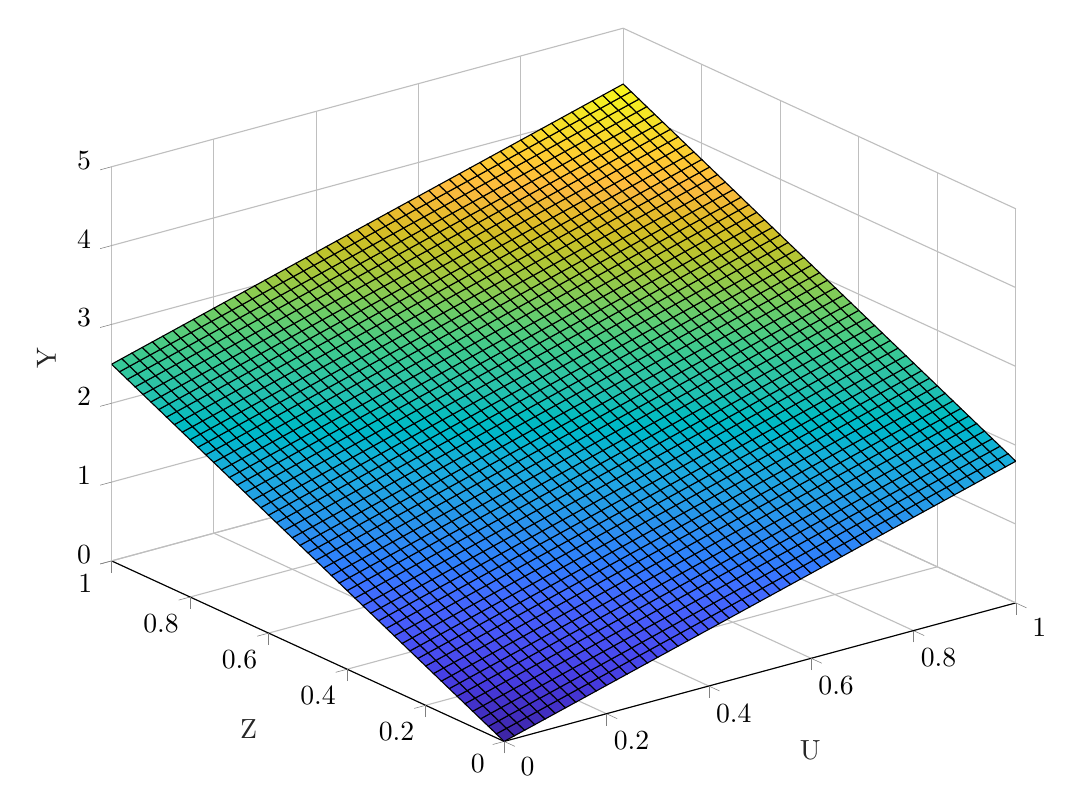
\begin{tikzpicture}

\begin{axis}[%
width=4.521in,
height=3.566in,
at={(0.758in,0.481in)},
scale only axis,
xmin=0,
xmax=1,
tick align=outside,
xlabel style={font=\color{white!15!black}},
xlabel={U},
ymin=0,
ymax=1,
ylabel style={font=\color{white!15!black}},
ylabel={Z},
zmin=0,
zmax=5,
zlabel style={font=\color{white!15!black}},
zlabel={Y},
view={-37.5}{30},
axis background/.style={fill=white},
axis x line*=bottom,
axis y line*=left,
axis z line*=left,
xmajorgrids,
ymajorgrids,
zmajorgrids
]

\addplot3[%
surf,
shader=flat corner, draw=black, z buffer=sort, colormap={mymap}{[1pt] rgb(0pt)=(0.2422,0.1504,0.6603); rgb(1pt)=(0.2444,0.1534,0.6728); rgb(2pt)=(0.2464,0.1569,0.6847); rgb(3pt)=(0.2484,0.1607,0.6961); rgb(4pt)=(0.2503,0.1648,0.7071); rgb(5pt)=(0.2522,0.1689,0.7179); rgb(6pt)=(0.254,0.1732,0.7286); rgb(7pt)=(0.2558,0.1773,0.7393); rgb(8pt)=(0.2576,0.1814,0.7501); rgb(9pt)=(0.2594,0.1854,0.761); rgb(11pt)=(0.2628,0.1932,0.7828); rgb(12pt)=(0.2645,0.1972,0.7937); rgb(13pt)=(0.2661,0.2011,0.8043); rgb(14pt)=(0.2676,0.2052,0.8148); rgb(15pt)=(0.2691,0.2094,0.8249); rgb(16pt)=(0.2704,0.2138,0.8346); rgb(17pt)=(0.2717,0.2184,0.8439); rgb(18pt)=(0.2729,0.2231,0.8528); rgb(19pt)=(0.274,0.228,0.8612); rgb(20pt)=(0.2749,0.233,0.8692); rgb(21pt)=(0.2758,0.2382,0.8767); rgb(22pt)=(0.2766,0.2435,0.884); rgb(23pt)=(0.2774,0.2489,0.8908); rgb(24pt)=(0.2781,0.2543,0.8973); rgb(25pt)=(0.2788,0.2598,0.9035); rgb(26pt)=(0.2794,0.2653,0.9094); rgb(27pt)=(0.2798,0.2708,0.915); rgb(28pt)=(0.2802,0.2764,0.9204); rgb(29pt)=(0.2806,0.2819,0.9255); rgb(30pt)=(0.2809,0.2875,0.9305); rgb(31pt)=(0.2811,0.293,0.9352); rgb(32pt)=(0.2813,0.2985,0.9397); rgb(33pt)=(0.2814,0.304,0.9441); rgb(34pt)=(0.2814,0.3095,0.9483); rgb(35pt)=(0.2813,0.315,0.9524); rgb(36pt)=(0.2811,0.3204,0.9563); rgb(37pt)=(0.2809,0.3259,0.96); rgb(38pt)=(0.2807,0.3313,0.9636); rgb(39pt)=(0.2803,0.3367,0.967); rgb(40pt)=(0.2798,0.3421,0.9702); rgb(41pt)=(0.2791,0.3475,0.9733); rgb(42pt)=(0.2784,0.3529,0.9763); rgb(43pt)=(0.2776,0.3583,0.9791); rgb(44pt)=(0.2766,0.3638,0.9817); rgb(45pt)=(0.2754,0.3693,0.984); rgb(46pt)=(0.2741,0.3748,0.9862); rgb(47pt)=(0.2726,0.3804,0.9881); rgb(48pt)=(0.271,0.386,0.9898); rgb(49pt)=(0.2691,0.3916,0.9912); rgb(50pt)=(0.267,0.3973,0.9924); rgb(51pt)=(0.2647,0.403,0.9935); rgb(52pt)=(0.2621,0.4088,0.9946); rgb(53pt)=(0.2591,0.4145,0.9955); rgb(54pt)=(0.2556,0.4203,0.9965); rgb(55pt)=(0.2517,0.4261,0.9974); rgb(56pt)=(0.2473,0.4319,0.9983); rgb(57pt)=(0.2424,0.4378,0.9991); rgb(58pt)=(0.2369,0.4437,0.9996); rgb(59pt)=(0.2311,0.4497,0.9995); rgb(60pt)=(0.225,0.4559,0.9985); rgb(61pt)=(0.2189,0.462,0.9968); rgb(62pt)=(0.2128,0.4682,0.9948); rgb(63pt)=(0.2066,0.4743,0.9926); rgb(64pt)=(0.2006,0.4803,0.9906); rgb(65pt)=(0.195,0.4861,0.9887); rgb(66pt)=(0.1903,0.4919,0.9867); rgb(67pt)=(0.1869,0.4975,0.9844); rgb(68pt)=(0.1847,0.503,0.9819); rgb(69pt)=(0.1831,0.5084,0.9793); rgb(70pt)=(0.1818,0.5138,0.9766); rgb(71pt)=(0.1806,0.5191,0.9738); rgb(72pt)=(0.1795,0.5244,0.9709); rgb(73pt)=(0.1785,0.5296,0.9677); rgb(74pt)=(0.1778,0.5349,0.9641); rgb(75pt)=(0.1773,0.5401,0.9602); rgb(76pt)=(0.1768,0.5452,0.956); rgb(77pt)=(0.1764,0.5504,0.9516); rgb(78pt)=(0.1755,0.5554,0.9473); rgb(79pt)=(0.174,0.5605,0.9432); rgb(80pt)=(0.1716,0.5655,0.9393); rgb(81pt)=(0.1686,0.5705,0.9357); rgb(82pt)=(0.1649,0.5755,0.9323); rgb(83pt)=(0.161,0.5805,0.9289); rgb(84pt)=(0.1573,0.5854,0.9254); rgb(85pt)=(0.154,0.5902,0.9218); rgb(86pt)=(0.1513,0.595,0.9182); rgb(87pt)=(0.1492,0.5997,0.9147); rgb(88pt)=(0.1475,0.6043,0.9113); rgb(89pt)=(0.1461,0.6089,0.908); rgb(90pt)=(0.1446,0.6135,0.905); rgb(91pt)=(0.1429,0.618,0.9022); rgb(92pt)=(0.1408,0.6226,0.8998); rgb(93pt)=(0.1383,0.6272,0.8975); rgb(94pt)=(0.1354,0.6317,0.8953); rgb(95pt)=(0.1321,0.6363,0.8932); rgb(96pt)=(0.1288,0.6408,0.891); rgb(97pt)=(0.1253,0.6453,0.8887); rgb(98pt)=(0.1219,0.6497,0.8862); rgb(99pt)=(0.1185,0.6541,0.8834); rgb(100pt)=(0.1152,0.6584,0.8804); rgb(101pt)=(0.1119,0.6627,0.877); rgb(102pt)=(0.1085,0.6669,0.8734); rgb(103pt)=(0.1048,0.671,0.8695); rgb(104pt)=(0.1009,0.675,0.8653); rgb(105pt)=(0.0964,0.6789,0.8609); rgb(106pt)=(0.0914,0.6828,0.8562); rgb(107pt)=(0.0855,0.6865,0.8513); rgb(108pt)=(0.0789,0.6902,0.8462); rgb(109pt)=(0.0713,0.6938,0.8409); rgb(110pt)=(0.0628,0.6972,0.8355); rgb(111pt)=(0.0535,0.7006,0.8299); rgb(112pt)=(0.0433,0.7039,0.8242); rgb(113pt)=(0.0328,0.7071,0.8183); rgb(114pt)=(0.0234,0.7103,0.8124); rgb(115pt)=(0.0155,0.7133,0.8064); rgb(116pt)=(0.0091,0.7163,0.8003); rgb(117pt)=(0.0046,0.7192,0.7941); rgb(118pt)=(0.0019,0.722,0.7878); rgb(119pt)=(0.0009,0.7248,0.7815); rgb(120pt)=(0.0018,0.7275,0.7752); rgb(121pt)=(0.0046,0.7301,0.7688); rgb(122pt)=(0.0094,0.7327,0.7623); rgb(123pt)=(0.0162,0.7352,0.7558); rgb(124pt)=(0.0253,0.7376,0.7492); rgb(125pt)=(0.0369,0.74,0.7426); rgb(126pt)=(0.0504,0.7423,0.7359); rgb(127pt)=(0.0638,0.7446,0.7292); rgb(128pt)=(0.077,0.7468,0.7224); rgb(129pt)=(0.0899,0.7489,0.7156); rgb(130pt)=(0.1023,0.751,0.7088); rgb(131pt)=(0.1141,0.7531,0.7019); rgb(132pt)=(0.1252,0.7552,0.695); rgb(133pt)=(0.1354,0.7572,0.6881); rgb(134pt)=(0.1448,0.7593,0.6812); rgb(135pt)=(0.1532,0.7614,0.6741); rgb(136pt)=(0.1609,0.7635,0.6671); rgb(137pt)=(0.1678,0.7656,0.6599); rgb(138pt)=(0.1741,0.7678,0.6527); rgb(139pt)=(0.1799,0.7699,0.6454); rgb(140pt)=(0.1853,0.7721,0.6379); rgb(141pt)=(0.1905,0.7743,0.6303); rgb(142pt)=(0.1954,0.7765,0.6225); rgb(143pt)=(0.2003,0.7787,0.6146); rgb(144pt)=(0.2061,0.7808,0.6065); rgb(145pt)=(0.2118,0.7828,0.5983); rgb(146pt)=(0.2178,0.7849,0.5899); rgb(147pt)=(0.2244,0.7869,0.5813); rgb(148pt)=(0.2318,0.7887,0.5725); rgb(149pt)=(0.2401,0.7905,0.5636); rgb(150pt)=(0.2491,0.7922,0.5546); rgb(151pt)=(0.2589,0.7937,0.5454); rgb(152pt)=(0.2695,0.7951,0.536); rgb(153pt)=(0.2809,0.7964,0.5266); rgb(154pt)=(0.2929,0.7975,0.517); rgb(155pt)=(0.3052,0.7985,0.5074); rgb(156pt)=(0.3176,0.7994,0.4975); rgb(157pt)=(0.3301,0.8002,0.4876); rgb(158pt)=(0.3424,0.8009,0.4774); rgb(159pt)=(0.3548,0.8016,0.4669); rgb(160pt)=(0.3671,0.8021,0.4563); rgb(161pt)=(0.3795,0.8026,0.4454); rgb(162pt)=(0.3921,0.8029,0.4344); rgb(163pt)=(0.405,0.8031,0.4233); rgb(164pt)=(0.4184,0.803,0.4122); rgb(165pt)=(0.4322,0.8028,0.4013); rgb(166pt)=(0.4463,0.8024,0.3904); rgb(167pt)=(0.4608,0.8018,0.3797); rgb(168pt)=(0.4753,0.8011,0.3691); rgb(169pt)=(0.4899,0.8002,0.3586); rgb(170pt)=(0.5044,0.7993,0.348); rgb(171pt)=(0.5187,0.7982,0.3374); rgb(172pt)=(0.5329,0.797,0.3267); rgb(173pt)=(0.547,0.7957,0.3159); rgb(175pt)=(0.5748,0.7929,0.2941); rgb(176pt)=(0.5886,0.7913,0.2833); rgb(177pt)=(0.6024,0.7896,0.2726); rgb(178pt)=(0.6161,0.7878,0.2622); rgb(179pt)=(0.6297,0.7859,0.2521); rgb(180pt)=(0.6433,0.7839,0.2423); rgb(181pt)=(0.6567,0.7818,0.2329); rgb(182pt)=(0.6701,0.7796,0.2239); rgb(183pt)=(0.6833,0.7773,0.2155); rgb(184pt)=(0.6963,0.775,0.2075); rgb(185pt)=(0.7091,0.7727,0.1998); rgb(186pt)=(0.7218,0.7703,0.1924); rgb(187pt)=(0.7344,0.7679,0.1852); rgb(188pt)=(0.7468,0.7654,0.1782); rgb(189pt)=(0.759,0.7629,0.1717); rgb(190pt)=(0.771,0.7604,0.1658); rgb(191pt)=(0.7829,0.7579,0.1608); rgb(192pt)=(0.7945,0.7554,0.157); rgb(193pt)=(0.806,0.7529,0.1546); rgb(194pt)=(0.8172,0.7505,0.1535); rgb(195pt)=(0.8281,0.7481,0.1536); rgb(196pt)=(0.8389,0.7457,0.1546); rgb(197pt)=(0.8495,0.7435,0.1564); rgb(198pt)=(0.86,0.7413,0.1587); rgb(199pt)=(0.8703,0.7392,0.1615); rgb(200pt)=(0.8804,0.7372,0.165); rgb(201pt)=(0.8903,0.7353,0.1695); rgb(202pt)=(0.9,0.7336,0.1749); rgb(203pt)=(0.9093,0.7321,0.1815); rgb(204pt)=(0.9184,0.7308,0.189); rgb(205pt)=(0.9272,0.7298,0.1973); rgb(206pt)=(0.9357,0.729,0.2061); rgb(207pt)=(0.944,0.7285,0.2151); rgb(208pt)=(0.9523,0.7284,0.2237); rgb(209pt)=(0.9606,0.7285,0.2312); rgb(210pt)=(0.9689,0.7292,0.2373); rgb(211pt)=(0.977,0.7304,0.2418); rgb(212pt)=(0.9842,0.733,0.2446); rgb(213pt)=(0.99,0.7365,0.2429); rgb(214pt)=(0.9946,0.7407,0.2394); rgb(215pt)=(0.9966,0.7458,0.2351); rgb(216pt)=(0.9971,0.7513,0.2309); rgb(217pt)=(0.9972,0.7569,0.2267); rgb(218pt)=(0.9971,0.7626,0.2224); rgb(219pt)=(0.9969,0.7683,0.2181); rgb(220pt)=(0.9966,0.774,0.2138); rgb(221pt)=(0.9962,0.7798,0.2095); rgb(222pt)=(0.9957,0.7856,0.2053); rgb(223pt)=(0.9949,0.7915,0.2012); rgb(224pt)=(0.9938,0.7974,0.1974); rgb(225pt)=(0.9923,0.8034,0.1939); rgb(226pt)=(0.9906,0.8095,0.1906); rgb(227pt)=(0.9885,0.8156,0.1875); rgb(228pt)=(0.9861,0.8218,0.1846); rgb(229pt)=(0.9835,0.828,0.1817); rgb(230pt)=(0.9807,0.8342,0.1787); rgb(231pt)=(0.9778,0.8404,0.1757); rgb(232pt)=(0.9748,0.8467,0.1726); rgb(233pt)=(0.972,0.8529,0.1695); rgb(234pt)=(0.9694,0.8591,0.1665); rgb(235pt)=(0.9671,0.8654,0.1636); rgb(236pt)=(0.9651,0.8716,0.1608); rgb(237pt)=(0.9634,0.8778,0.1582); rgb(238pt)=(0.9619,0.884,0.1557); rgb(239pt)=(0.9608,0.8902,0.1532); rgb(240pt)=(0.9601,0.8963,0.1507); rgb(241pt)=(0.9596,0.9023,0.148); rgb(242pt)=(0.9595,0.9084,0.145); rgb(243pt)=(0.9597,0.9143,0.1418); rgb(244pt)=(0.9601,0.9203,0.1382); rgb(245pt)=(0.9608,0.9262,0.1344); rgb(246pt)=(0.9618,0.932,0.1304); rgb(247pt)=(0.9629,0.9379,0.1261); rgb(248pt)=(0.9642,0.9437,0.1216); rgb(249pt)=(0.9657,0.9494,0.1168); rgb(250pt)=(0.9674,0.9552,0.1116); rgb(251pt)=(0.9692,0.9609,0.1061); rgb(252pt)=(0.9711,0.9667,0.1001); rgb(253pt)=(0.973,0.9724,0.0938); rgb(254pt)=(0.9749,0.9782,0.0872); rgb(255pt)=(0.9769,0.9839,0.0805)}, mesh/rows=51]
table[row sep=crcr, point meta=\thisrow{c}] {%
%
x	y	z	c\\
0	0	0	0\\
0	0.02	0.0498947354210309	0.0498947354210309\\
0	0.04	0.0997894708420618	0.0997894708420618\\
0	0.06	0.149684206263086	0.149684206263086\\
0	0.08	0.199578941684124	0.199578941684124\\
0	0.1	0.24947367710515	0.24947367710515\\
0	0.12	0.299368412526172	0.299368412526172\\
0	0.14	0.349263147947199	0.349263147947199\\
0	0.16	0.399157883368247	0.399157883368247\\
0	0.18	0.449052618789275	0.449052618789275\\
0	0.2	0.498947354210301	0.498947354210301\\
0	0.22	0.54884208963133	0.54884208963133\\
0	0.24	0.598736825052343	0.598736825052343\\
0	0.26	0.648631560473387	0.648631560473387\\
0	0.28	0.698526295894397	0.698526295894397\\
0	0.3	0.748421031315445	0.748421031315445\\
0	0.32	0.798315766736494	0.798315766736494\\
0	0.34	0.848210502157503	0.848210502157503\\
0	0.36	0.89810523757855	0.89810523757855\\
0	0.38	0.947999972999557	0.947999972999557\\
0	0.4	0.997894708420602	0.997894708420602\\
0	0.42	1.04778944384161	1.04778944384161\\
0	0.44	1.09768417926266	1.09768417926266\\
0	0.46	1.1475789146837	1.1475789146837\\
0	0.48	1.19747365010469	1.19747365010469\\
0	0.5	1.24736838552573	1.24736838552573\\
0	0.52	1.29726312094677	1.29726312094677\\
0	0.54	1.34715785636782	1.34715785636782\\
0	0.56	1.39705259178879	1.39705259178879\\
0	0.58	1.44694732720984	1.44694732720984\\
0	0.6	1.49684206263089	1.49684206263089\\
0	0.62	1.54673679805193	1.54673679805193\\
0	0.64	1.59663153347299	1.59663153347299\\
0	0.66	1.64652626889396	1.64652626889396\\
0	0.68	1.69642100431501	1.69642100431501\\
0	0.7	1.74631573973605	1.74631573973605\\
0	0.72	1.7962104751571	1.7962104751571\\
0	0.74	1.84610521057807	1.84610521057807\\
0	0.76	1.89599994599911	1.89599994599911\\
0	0.78	1.94589468142017	1.94589468142017\\
0	0.8	1.9957894168412	1.9957894168412\\
0	0.82	2.04568415226218	2.04568415226218\\
0	0.84	2.09557888768323	2.09557888768323\\
0	0.86	2.14547362310429	2.14547362310429\\
0	0.88	2.19536835852532	2.19536835852532\\
0	0.9	2.2452630939463	2.2452630939463\\
0	0.92	2.2951578293674	2.2951578293674\\
0	0.94	2.34505256478839	2.34505256478839\\
0	0.96	2.39494730020937	2.39494730020937\\
0	0.98	2.44484203563049	2.44484203563049\\
0	1	2.49473677105147	2.49473677105147\\
0.02	0	0.0359398496296482	0.0359398496296482\\
0.02	0.02	0.0858345850506791	0.0858345850506791\\
0.02	0.04	0.135729320471707	0.135729320471707\\
0.02	0.06	0.18562405589274	0.18562405589274\\
0.02	0.08	0.235518791313768	0.235518791313768\\
0.02	0.1	0.285413526734789	0.285413526734789\\
0.02	0.12	0.335308262155818	0.335308262155818\\
0.02	0.14	0.385202997576862	0.385202997576862\\
0.02	0.16	0.435097732997891	0.435097732997891\\
0.02	0.18	0.48499246841892	0.48499246841892\\
0.02	0.2	0.534887203839948	0.534887203839948\\
0.02	0.22	0.584781939260962	0.584781939260962\\
0.02	0.24	0.634676674682009	0.634676674682009\\
0.02	0.26	0.684571410103016	0.684571410103016\\
0.02	0.28	0.734466145524064	0.734466145524064\\
0.02	0.3	0.784360880945109	0.784360880945109\\
0.02	0.32	0.834255616366123	0.834255616366123\\
0.02	0.34	0.884150351787166	0.884150351787166\\
0.02	0.36	0.934045087208179	0.934045087208179\\
0.02	0.38	0.983939822629225	0.983939822629225\\
0.02	0.4	1.03383455805024	1.03383455805024\\
0.02	0.42	1.08372929347128	1.08372929347128\\
0.02	0.44	1.13362402889233	1.13362402889233\\
0.02	0.46	1.1835187643133	1.1835187643133\\
0.02	0.48	1.23341349973435	1.23341349973435\\
0.02	0.5	1.2833082351554	1.2833082351554\\
0.02	0.52	1.33320297057644	1.33320297057644\\
0.02	0.54	1.38309770599742	1.38309770599742\\
0.02	0.56	1.43299244141846	1.43299244141846\\
0.02	0.58	1.48288717683951	1.48288717683951\\
0.02	0.6	1.53278191226055	1.53278191226055\\
0.02	0.62	1.5826766476816	1.5826766476816\\
0.02	0.64	1.63257138310258	1.63257138310258\\
0.02	0.66	1.68246611852362	1.68246611852362\\
0.02	0.68	1.73236085394467	1.73236085394467\\
0.02	0.7	1.78225558936571	1.78225558936571\\
0.02	0.72	1.83215032478669	1.83215032478669\\
0.02	0.74	1.88204506020774	1.88204506020774\\
0.02	0.76	1.93193979562878	1.93193979562878\\
0.02	0.78	1.98183453104982	1.98183453104982\\
0.02	0.8	2.03172926647081	2.03172926647081\\
0.02	0.82	2.08162400189185	2.08162400189185\\
0.02	0.84	2.13151873731289	2.13151873731289\\
0.02	0.86	2.18141347273392	2.18141347273392\\
0.02	0.88	2.23130820815492	2.23130820815492\\
0.02	0.9	2.28120294357604	2.28120294357604\\
0.02	0.92	2.331097678997	2.331097678997\\
0.02	0.94	2.38099241441798	2.38099241441798\\
0.02	0.96	2.43088714983909	2.43088714983909\\
0.02	0.98	2.48078188526008	2.48078188526008\\
0.02	1	2.53067662068118	2.53067662068118\\
0.04	0	0.0718796992592964	0.0718796992592964\\
0.04	0.02	0.121774434680325	0.121774434680325\\
0.04	0.04	0.171669170101358	0.171669170101358\\
0.04	0.06	0.221563905522386	0.221563905522386\\
0.04	0.08	0.271458640943414	0.271458640943414\\
0.04	0.1	0.321353376364454	0.321353376364454\\
0.04	0.12	0.37124811178548	0.37124811178548\\
0.04	0.14	0.421142847206508	0.421142847206508\\
0.04	0.16	0.471037582627537	0.471037582627537\\
0.04	0.18	0.520932318048566	0.520932318048566\\
0.04	0.2	0.570827053469578	0.570827053469578\\
0.04	0.22	0.620721788890622	0.620721788890622\\
0.04	0.24	0.670616524311637	0.670616524311637\\
0.04	0.26	0.720511259732681	0.720511259732681\\
0.04	0.28	0.770405995153724	0.770405995153724\\
0.04	0.3	0.820300730574741	0.820300730574741\\
0.04	0.32	0.870195465995782	0.870195465995782\\
0.04	0.34	0.920090201416796	0.920090201416796\\
0.04	0.36	0.96998493683784	0.96998493683784\\
0.04	0.38	1.01987967225885	1.01987967225885\\
0.04	0.4	1.0697744076799	1.0697744076799\\
0.04	0.42	1.11966914310094	1.11966914310094\\
0.04	0.44	1.16956387852192	1.16956387852192\\
0.04	0.46	1.21945861394297	1.21945861394297\\
0.04	0.48	1.26935334936402	1.26935334936402\\
0.04	0.5	1.31924808478506	1.31924808478506\\
0.04	0.52	1.36914282020603	1.36914282020603\\
0.04	0.54	1.41903755562708	1.41903755562708\\
0.04	0.56	1.46893229104813	1.46893229104813\\
0.04	0.58	1.51882702646917	1.51882702646917\\
0.04	0.6	1.56872176189022	1.56872176189022\\
0.04	0.62	1.61861649731119	1.61861649731119\\
0.04	0.64	1.66851123273225	1.66851123273225\\
0.04	0.66	1.71840596815329	1.71840596815329\\
0.04	0.68	1.76830070357433	1.76830070357433\\
0.04	0.7	1.81819543899531	1.81819543899531\\
0.04	0.72	1.86809017441636	1.86809017441636\\
0.04	0.74	1.9179849098374	1.9179849098374\\
0.04	0.76	1.96787964525845	1.96787964525845\\
0.04	0.78	2.01777438067942	2.01777438067942\\
0.04	0.8	2.06766911610047	2.06766911610047\\
0.04	0.82	2.11756385152151	2.11756385152151\\
0.04	0.84	2.16745858694257	2.16745858694257\\
0.04	0.86	2.21735332236354	2.21735332236354\\
0.04	0.88	2.26724805778466	2.26724805778466\\
0.04	0.9	2.31714279320562	2.31714279320562\\
0.04	0.92	2.36703752862661	2.36703752862661\\
0.04	0.94	2.41693226404771	2.41693226404771\\
0.04	0.96	2.46682699946871	2.46682699946871\\
0.04	0.98	2.51672173488981	2.51672173488981\\
0.04	1	2.56661647031079	2.56661647031079\\
0.06	0	0.107819548888943	0.107819548888943\\
0.06	0.02	0.157714284309976	0.157714284309976\\
0.06	0.04	0.207609019731004	0.207609019731004\\
0.06	0.06	0.257503755152033	0.257503755152033\\
0.06	0.08	0.307398490573069	0.307398490573069\\
0.06	0.1	0.357293225994098	0.357293225994098\\
0.06	0.12	0.407187961415128	0.407187961415128\\
0.06	0.14	0.457082696836156	0.457082696836156\\
0.06	0.16	0.506977432257185	0.506977432257185\\
0.06	0.18	0.556872167678197	0.556872167678197\\
0.06	0.2	0.60676690309924	0.60676690309924\\
0.06	0.22	0.656661638520288	0.656661638520288\\
0.06	0.24	0.706556373941299	0.706556373941299\\
0.06	0.26	0.756451109362345	0.756451109362345\\
0.06	0.28	0.806345844783356	0.806345844783356\\
0.06	0.3	0.856240580204401	0.856240580204401\\
0.06	0.32	0.906135315625411	0.906135315625411\\
0.06	0.34	0.956030051046457	0.956030051046457\\
0.06	0.36	1.00592478646747	1.00592478646747\\
0.06	0.38	1.05581952188851	1.05581952188851\\
0.06	0.4	1.10571425730956	1.10571425730956\\
0.06	0.42	1.15560899273054	1.15560899273054\\
0.06	0.44	1.20550372815158	1.20550372815158\\
0.06	0.46	1.25539846357263	1.25539846357263\\
0.06	0.48	1.30529319899368	1.30529319899368\\
0.06	0.5	1.35518793441466	1.35518793441466\\
0.06	0.52	1.40508266983569	1.40508266983569\\
0.06	0.54	1.45497740525675	1.45497740525675\\
0.06	0.56	1.50487214067779	1.50487214067779\\
0.06	0.58	1.55476687609883	1.55476687609883\\
0.06	0.6	1.60466161151981	1.60466161151981\\
0.06	0.62	1.65455634694086	1.65455634694086\\
0.06	0.64	1.7044510823619	1.7044510823619\\
0.06	0.66	1.75434581778294	1.75434581778294\\
0.06	0.68	1.80424055320392	1.80424055320392\\
0.06	0.7	1.85413528862497	1.85413528862497\\
0.06	0.72	1.90403002404602	1.90403002404602\\
0.06	0.74	1.95392475946707	1.95392475946707\\
0.06	0.76	2.00381949488804	2.00381949488804\\
0.06	0.78	2.05371423030908	2.05371423030908\\
0.06	0.8	2.10360896573013	2.10360896573013\\
0.06	0.82	2.15350370115117	2.15350370115117\\
0.06	0.84	2.20339843657216	2.20339843657216\\
0.06	0.86	2.25329317199327	2.25329317199327\\
0.06	0.88	2.30318790741425	2.30318790741425\\
0.06	0.9	2.35308264283522	2.35308264283522\\
0.06	0.92	2.40297737825633	2.40297737825633\\
0.06	0.94	2.45287211367732	2.45287211367732\\
0.06	0.96	2.50276684909843	2.50276684909843\\
0.06	0.98	2.5526615845194	2.5526615845194\\
0.06	1	2.60255631994038	2.60255631994038\\
0.08	0	0.143759398518593	0.143759398518593\\
0.08	0.02	0.193654133939622	0.193654133939622\\
0.08	0.04	0.24354886936065	0.24354886936065\\
0.08	0.06	0.293443604781686	0.293443604781686\\
0.08	0.08	0.343338340202716	0.343338340202716\\
0.08	0.1	0.393233075623744	0.393233075623744\\
0.08	0.12	0.443127811044772	0.443127811044772\\
0.08	0.14	0.493022546465801	0.493022546465801\\
0.08	0.16	0.542917281886829	0.542917281886829\\
0.08	0.18	0.592812017307857	0.592812017307857\\
0.08	0.2	0.642706752728908	0.642706752728908\\
0.08	0.22	0.692601488149914	0.692601488149914\\
0.08	0.24	0.74249622357096	0.74249622357096\\
0.08	0.26	0.792390958991971	0.792390958991971\\
0.08	0.28	0.842285694413017	0.842285694413017\\
0.08	0.3	0.89218042983403	0.89218042983403\\
0.08	0.32	0.942075165255074	0.942075165255074\\
0.08	0.34	0.991969900676089	0.991969900676089\\
0.08	0.36	1.04186463609713	1.04186463609713\\
0.08	0.38	1.09175937151816	1.09175937151816\\
0.08	0.4	1.14165410693916	1.14165410693916\\
0.08	0.42	1.1915488423602	1.1915488423602\\
0.08	0.44	1.24144357778124	1.24144357778124\\
0.08	0.46	1.29133831320229	1.29133831320229\\
0.08	0.48	1.34123304862327	1.34123304862327\\
0.08	0.5	1.39112778404432	1.39112778404432\\
0.08	0.52	1.44102251946536	1.44102251946536\\
0.08	0.54	1.49091725488641	1.49091725488641\\
0.08	0.56	1.54081199030745	1.54081199030745\\
0.08	0.58	1.59070672572844	1.59070672572844\\
0.08	0.6	1.64060146114948	1.64060146114948\\
0.08	0.62	1.69049619657052	1.69049619657052\\
0.08	0.64	1.74039093199156	1.74039093199156\\
0.08	0.66	1.79028566741254	1.79028566741254\\
0.08	0.68	1.84018040283359	1.84018040283359\\
0.08	0.7	1.89007513825463	1.89007513825463\\
0.08	0.72	1.93996987367568	1.93996987367568\\
0.08	0.74	1.98986460909666	1.98986460909666\\
0.08	0.76	2.03975934451771	2.03975934451771\\
0.08	0.78	2.08965407993875	2.08965407993875\\
0.08	0.8	2.13954881535979	2.13954881535979\\
0.08	0.82	2.18944355078078	2.18944355078078\\
0.08	0.84	2.23933828620189	2.23933828620189\\
0.08	0.86	2.28923302162286	2.28923302162286\\
0.08	0.88	2.33912775704385	2.33912775704385\\
0.08	0.9	2.38902249246496	2.38902249246496\\
0.08	0.92	2.43891722788594	2.43891722788594\\
0.08	0.94	2.48881196330703	2.48881196330703\\
0.08	0.96	2.53870669872803	2.53870669872803\\
0.08	0.98	2.588601434149	2.588601434149\\
0.08	1	2.63849616957011	2.63849616957011\\
0.1	0	0.17969924814824	0.17969924814824\\
0.1	0.02	0.229593983569269	0.229593983569269\\
0.1	0.04	0.279488718990304	0.279488718990304\\
0.1	0.06	0.329383454411333	0.329383454411333\\
0.1	0.08	0.379278189832362	0.379278189832362\\
0.1	0.1	0.429172925253391	0.429172925253391\\
0.1	0.12	0.479067660674419	0.479067660674419\\
0.1	0.14	0.528962396095447	0.528962396095447\\
0.1	0.16	0.578857131516475	0.578857131516475\\
0.1	0.18	0.628751866937525	0.628751866937525\\
0.1	0.2	0.678646602358533	0.678646602358533\\
0.1	0.22	0.728541337779578	0.728541337779578\\
0.1	0.24	0.778436073200591	0.778436073200591\\
0.1	0.26	0.828330808621635	0.828330808621635\\
0.1	0.28	0.878225544042649	0.878225544042649\\
0.1	0.3	0.928120279463694	0.928120279463694\\
0.1	0.32	0.978015014884705	0.978015014884705\\
0.1	0.34	1.02790975030575	1.02790975030575\\
0.1	0.36	1.07780448572677	1.07780448572677\\
0.1	0.38	1.12769922114777	1.12769922114777\\
0.1	0.4	1.17759395656881	1.17759395656881\\
0.1	0.42	1.22748869198986	1.22748869198986\\
0.1	0.44	1.27738342741091	1.27738342741091\\
0.1	0.46	1.32727816283192	1.32727816283192\\
0.1	0.48	1.37717289825294	1.37717289825294\\
0.1	0.5	1.42706763367398	1.42706763367398\\
0.1	0.52	1.47696236909502	1.47696236909502\\
0.1	0.54	1.52685710451607	1.52685710451607\\
0.1	0.56	1.57675183993705	1.57675183993705\\
0.1	0.58	1.62664657535809	1.62664657535809\\
0.1	0.6	1.67654131077914	1.67654131077914\\
0.1	0.62	1.72643604620018	1.72643604620018\\
0.1	0.64	1.77633078162117	1.77633078162117\\
0.1	0.66	1.82622551704221	1.82622551704221\\
0.1	0.68	1.87612025246325	1.87612025246325\\
0.1	0.7	1.9260149878843	1.9260149878843\\
0.1	0.72	1.97590972330528	1.97590972330528\\
0.1	0.74	2.02580445872632	2.02580445872632\\
0.1	0.76	2.07569919414737	2.07569919414737\\
0.1	0.78	2.12559392956841	2.12559392956841\\
0.1	0.8	2.17548866498947	2.17548866498947\\
0.1	0.82	2.22538340041049	2.22538340041049\\
0.1	0.84	2.27527813583149	2.27527813583149\\
0.1	0.86	2.32517287125244	2.32517287125244\\
0.1	0.88	2.37506760667358	2.37506760667358\\
0.1	0.9	2.42496234209455	2.42496234209455\\
0.1	0.92	2.47485707751565	2.47485707751565\\
0.1	0.94	2.52475181293664	2.52475181293664\\
0.1	0.96	2.57464654835761	2.57464654835761\\
0.1	0.98	2.62454128377873	2.62454128377873\\
0.1	1	2.67443601919971	2.67443601919971\\
0.12	0	0.215639097777886	0.215639097777886\\
0.12	0.02	0.265533833198914	0.265533833198914\\
0.12	0.04	0.315428568619951	0.315428568619951\\
0.12	0.06	0.36532330404098	0.36532330404098\\
0.12	0.08	0.415218039462009	0.415218039462009\\
0.12	0.1	0.465112774883036	0.465112774883036\\
0.12	0.12	0.515007510304066	0.515007510304066\\
0.12	0.14	0.564902245725092	0.564902245725092\\
0.12	0.16	0.614796981146138	0.614796981146138\\
0.12	0.18	0.664691716567152	0.664691716567152\\
0.12	0.2	0.714586451988197	0.714586451988197\\
0.12	0.22	0.764481187409209	0.764481187409209\\
0.12	0.24	0.814375922830255	0.814375922830255\\
0.12	0.26	0.864270658251266	0.864270658251266\\
0.12	0.28	0.914165393672312	0.914165393672312\\
0.12	0.3	0.964060129093322	0.964060129093322\\
0.12	0.32	1.01395486451437	1.01395486451437\\
0.12	0.34	1.06384959993538	1.06384959993538\\
0.12	0.36	1.11374433535639	1.11374433535639\\
0.12	0.38	1.16363907077744	1.16363907077744\\
0.12	0.4	1.21353380619848	1.21353380619848\\
0.12	0.42	1.26342854161953	1.26342854161953\\
0.12	0.44	1.31332327704058	1.31332327704058\\
0.12	0.46	1.36321801246155	1.36321801246155\\
0.12	0.48	1.4131127478826	1.4131127478826\\
0.12	0.5	1.46300748330365	1.46300748330365\\
0.12	0.52	1.51290221872469	1.51290221872469\\
0.12	0.54	1.56279695414566	1.56279695414566\\
0.12	0.56	1.61269168956671	1.61269168956671\\
0.12	0.58	1.66258642498776	1.66258642498776\\
0.12	0.6	1.7124811604088	1.7124811604088\\
0.12	0.62	1.76237589582978	1.76237589582978\\
0.12	0.64	1.81227063125082	1.81227063125082\\
0.12	0.66	1.86216536667187	1.86216536667187\\
0.12	0.68	1.91206010209291	1.91206010209291\\
0.12	0.7	1.96195483751389	1.96195483751389\\
0.12	0.72	2.01184957293495	2.01184957293495\\
0.12	0.74	2.06174430835598	2.06174430835598\\
0.12	0.76	2.11163904377703	2.11163904377703\\
0.12	0.78	2.16153377919807	2.16153377919807\\
0.12	0.8	2.21142851461912	2.21142851461912\\
0.12	0.82	2.26132325004009	2.26132325004009\\
0.12	0.84	2.31121798546107	2.31121798546107\\
0.12	0.86	2.3611127208822	2.3611127208822\\
0.12	0.88	2.41100745630317	2.41100745630317\\
0.12	0.9	2.46090219172429	2.46090219172429\\
0.12	0.92	2.51079692714527	2.51079692714527\\
0.12	0.94	2.56069166256625	2.56069166256625\\
0.12	0.96	2.61058639798736	2.61058639798736\\
0.12	0.98	2.66048113340833	2.66048113340833\\
0.12	1	2.71037586882931	2.71037586882931\\
0.14	0	0.251578947407532	0.251578947407532\\
0.14	0.02	0.301473682828568	0.301473682828568\\
0.14	0.04	0.351368418249597	0.351368418249597\\
0.14	0.06	0.401263153670626	0.401263153670626\\
0.14	0.08	0.451157889091654	0.451157889091654\\
0.14	0.1	0.501052624512681	0.501052624512681\\
0.14	0.12	0.550947359933715	0.550947359933715\\
0.14	0.14	0.600842095354757	0.600842095354757\\
0.14	0.16	0.650736830775767	0.650736830775767\\
0.14	0.18	0.700631566196814	0.700631566196814\\
0.14	0.2	0.750526301617825	0.750526301617825\\
0.14	0.22	0.80042103703887	0.80042103703887\\
0.14	0.24	0.850315772459882	0.850315772459882\\
0.14	0.26	0.900210507880928	0.900210507880928\\
0.14	0.28	0.95010524330194	0.95010524330194\\
0.14	0.3	0.999999978722985	0.999999978722985\\
0.14	0.32	1.049894714144	1.049894714144\\
0.14	0.34	1.09978944956501	1.09978944956501\\
0.14	0.36	1.14968418498605	1.14968418498605\\
0.14	0.38	1.1995789204071	1.1995789204071\\
0.14	0.4	1.24947365582815	1.24947365582815\\
0.14	0.42	1.29936839124919	1.29936839124919\\
0.14	0.44	1.34926312667017	1.34926312667017\\
0.14	0.46	1.39915786209121	1.39915786209121\\
0.14	0.48	1.44905259751227	1.44905259751227\\
0.14	0.5	1.4989473329333	1.4989473329333\\
0.14	0.52	1.54884206835429	1.54884206835429\\
0.14	0.54	1.59873680377532	1.59873680377532\\
0.14	0.56	1.64863153919637	1.64863153919637\\
0.14	0.58	1.69852627461742	1.69852627461742\\
0.14	0.6	1.7484210100384	1.7484210100384\\
0.14	0.62	1.79831574545944	1.79831574545944\\
0.14	0.64	1.84821048088049	1.84821048088049\\
0.14	0.66	1.89810521630153	1.89810521630153\\
0.14	0.68	1.94799995172252	1.94799995172252\\
0.14	0.7	1.99789468714356	1.99789468714356\\
0.14	0.72	2.0477894225646	2.0477894225646\\
0.14	0.74	2.09768415798565	2.09768415798565\\
0.14	0.76	2.1475788934067	2.1475788934067\\
0.14	0.78	2.19747362882773	2.19747362882773\\
0.14	0.8	2.24736836424871	2.24736836424871\\
0.14	0.82	2.29726309966969	2.29726309966969\\
0.14	0.84	2.34715783509081	2.34715783509081\\
0.14	0.86	2.39705257051177	2.39705257051177\\
0.14	0.88	2.4469473059329	2.4469473059329\\
0.14	0.9	2.49684204135388	2.49684204135388\\
0.14	0.92	2.54673677677486	2.54673677677486\\
0.14	0.94	2.59663151219596	2.59663151219596\\
0.14	0.96	2.64652624761694	2.64652624761694\\
0.14	0.98	2.69642098303792	2.69642098303792\\
0.14	1	2.74631571845903	2.74631571845903\\
0.16	0	0.287518797037185	0.287518797037185\\
0.16	0.02	0.337413532458215	0.337413532458215\\
0.16	0.04	0.387308267879243	0.387308267879243\\
0.16	0.06	0.437203003300272	0.437203003300272\\
0.16	0.08	0.487097738721301	0.487097738721301\\
0.16	0.1	0.536992474142329	0.536992474142329\\
0.16	0.12	0.586887209563372	0.586887209563372\\
0.16	0.14	0.636781944984388	0.636781944984388\\
0.16	0.16	0.686676680405433	0.686676680405433\\
0.16	0.18	0.736571415826446	0.736571415826446\\
0.16	0.2	0.786466151247487	0.786466151247487\\
0.16	0.22	0.836360886668504	0.836360886668504\\
0.16	0.24	0.886255622089544	0.886255622089544\\
0.16	0.26	0.936150357510556	0.936150357510556\\
0.16	0.28	0.986045092931602	0.986045092931602\\
0.16	0.3	1.03593982835262	1.03593982835262\\
0.16	0.32	1.08583456377366	1.08583456377366\\
0.16	0.34	1.13572929919468	1.13572929919468\\
0.16	0.36	1.18562403461571	1.18562403461571\\
0.16	0.38	1.23551877003677	1.23551877003677\\
0.16	0.4	1.28541350545782	1.28541350545782\\
0.16	0.42	1.33530824087879	1.33530824087879\\
0.16	0.44	1.38520297629983	1.38520297629983\\
0.16	0.46	1.43509771172088	1.43509771172088\\
0.16	0.48	1.48499244714192	1.48499244714192\\
0.16	0.5	1.5348871825629	1.5348871825629\\
0.16	0.52	1.58478191798394	1.58478191798394\\
0.16	0.54	1.63467665340499	1.63467665340499\\
0.16	0.56	1.68457138882603	1.68457138882603\\
0.16	0.58	1.73446612424702	1.73446612424702\\
0.16	0.6	1.78436085966806	1.78436085966806\\
0.16	0.62	1.8342555950891	1.8342555950891\\
0.16	0.64	1.88415033051015	1.88415033051015\\
0.16	0.66	1.93404506593113	1.93404506593113\\
0.16	0.68	1.98393980135218	1.98393980135218\\
0.16	0.7	2.03383453677322	2.03383453677322\\
0.16	0.72	2.08372927219426	2.08372927219426\\
0.16	0.74	2.13362400761531	2.13362400761531\\
0.16	0.76	2.18351874303632	2.18351874303632\\
0.16	0.78	2.23341347845733	2.23341347845733\\
0.16	0.8	2.28330821387831	2.28330821387831\\
0.16	0.82	2.33320294929942	2.33320294929942\\
0.16	0.84	2.3830976847204	2.3830976847204\\
0.16	0.86	2.43299242014151	2.43299242014151\\
0.16	0.88	2.48288715556249	2.48288715556249\\
0.16	0.9	2.53278189098348	2.53278189098348\\
0.16	0.92	2.58267662640459	2.58267662640459\\
0.16	0.94	2.63257136182556	2.63257136182556\\
0.16	0.96	2.68246609724655	2.68246609724655\\
0.16	0.98	2.73236083266766	2.73236083266766\\
0.16	1	2.78225556808863	2.78225556808863\\
0.18	0	0.323458646666834	0.323458646666834\\
0.18	0.02	0.373353382087861	0.373353382087861\\
0.18	0.04	0.42324811750889	0.42324811750889\\
0.18	0.06	0.473142852929918	0.473142852929918\\
0.18	0.08	0.523037588350947	0.523037588350947\\
0.18	0.1	0.57293232377199	0.57293232377199\\
0.18	0.12	0.622827059193003	0.622827059193003\\
0.18	0.14	0.67272179461405	0.67272179461405\\
0.18	0.16	0.722616530035063	0.722616530035063\\
0.18	0.18	0.772511265456106	0.772511265456106\\
0.18	0.2	0.822406000877117	0.822406000877117\\
0.18	0.22	0.872300736298165	0.872300736298165\\
0.18	0.24	0.922195471719174	0.922195471719174\\
0.18	0.26	0.97209020714022	0.97209020714022\\
0.18	0.28	1.02198494256123	1.02198494256123\\
0.18	0.3	1.07187967798228	1.07187967798228\\
0.18	0.32	1.12177441340328	1.12177441340328\\
0.18	0.34	1.17166914882433	1.17166914882433\\
0.18	0.36	1.22156388424538	1.22156388424538\\
0.18	0.38	1.27145861966643	1.27145861966643\\
0.18	0.4	1.3213533550874	1.3213533550874\\
0.18	0.42	1.37124809050845	1.37124809050845\\
0.18	0.44	1.42114282592949	1.42114282592949\\
0.18	0.46	1.47103756135054	1.47103756135054\\
0.18	0.48	1.52093229677152	1.52093229677152\\
0.18	0.5	1.57082703219257	1.57082703219257\\
0.18	0.52	1.62072176761361	1.62072176761361\\
0.18	0.54	1.67061650303466	1.67061650303466\\
0.18	0.56	1.72051123845563	1.72051123845563\\
0.18	0.58	1.77040597387668	1.77040597387668\\
0.18	0.6	1.82030070929772	1.82030070929772\\
0.18	0.62	1.87019544471877	1.87019544471877\\
0.18	0.64	1.92009018013981	1.92009018013981\\
0.18	0.66	1.96998491556079	1.96998491556079\\
0.18	0.68	2.01987965098184	2.01987965098184\\
0.18	0.7	2.06977438640288	2.06977438640288\\
0.18	0.72	2.11966912182393	2.11966912182393\\
0.18	0.74	2.16956385724491	2.16956385724491\\
0.18	0.76	2.21945859266595	2.21945859266595\\
0.18	0.78	2.26935332808694	2.26935332808694\\
0.18	0.8	2.31924806350803	2.31924806350803\\
0.18	0.82	2.36914279892902	2.36914279892902\\
0.18	0.84	2.41903753435012	2.41903753435012\\
0.18	0.86	2.46893226977112	2.46893226977112\\
0.18	0.88	2.51882700519209	2.51882700519209\\
0.18	0.9	2.5687217406132	2.5687217406132\\
0.18	0.92	2.61861647603418	2.61861647603418\\
0.18	0.94	2.66851121145529	2.66851121145529\\
0.18	0.96	2.71840594687627	2.71840594687627\\
0.18	0.98	2.76830068229725	2.76830068229725\\
0.18	1	2.81819541771836	2.81819541771836\\
0.2	0	0.35939849629648	0.35939849629648\\
0.2	0.02	0.409293231717508	0.409293231717508\\
0.2	0.04	0.459187967138537	0.459187967138537\\
0.2	0.06	0.509082702559566	0.509082702559566\\
0.2	0.08	0.558977437980608	0.558977437980608\\
0.2	0.1	0.608872173401624	0.608872173401624\\
0.2	0.12	0.658766908822667	0.658766908822667\\
0.2	0.14	0.708661644243679	0.708661644243679\\
0.2	0.16	0.758556379664723	0.758556379664723\\
0.2	0.18	0.808451115085734	0.808451115085734\\
0.2	0.2	0.858345850506782	0.858345850506782\\
0.2	0.22	0.908240585927793	0.908240585927793\\
0.2	0.24	0.958135321348838	0.958135321348838\\
0.2	0.26	1.00803005676985	1.00803005676985\\
0.2	0.28	1.05792479219089	1.05792479219089\\
0.2	0.3	1.10781952761191	1.10781952761191\\
0.2	0.32	1.15771426303295	1.15771426303295\\
0.2	0.34	1.207608998454	1.207608998454\\
0.2	0.36	1.25750373387505	1.25750373387505\\
0.2	0.38	1.30739846929602	1.30739846929602\\
0.2	0.4	1.35729320471707	1.35729320471707\\
0.2	0.42	1.40718794013811	1.40718794013811\\
0.2	0.44	1.45708267555916	1.45708267555916\\
0.2	0.46	1.50697741098014	1.50697741098014\\
0.2	0.48	1.55687214640118	1.55687214640118\\
0.2	0.5	1.60676688182223	1.60676688182223\\
0.2	0.52	1.65666161724327	1.65666161724327\\
0.2	0.54	1.70655635266425	1.70655635266425\\
0.2	0.56	1.7564510880853	1.7564510880853\\
0.2	0.58	1.80634582350635	1.80634582350635\\
0.2	0.6	1.85624055892739	1.85624055892739\\
0.2	0.62	1.9061352943484	1.9061352943484\\
0.2	0.64	1.95603002976941	1.95603002976941\\
0.2	0.66	2.00592476519046	2.00592476519046\\
0.2	0.68	2.0558195006115	2.0558195006115\\
0.2	0.7	2.10571423603255	2.10571423603255\\
0.2	0.72	2.15560897145353	2.15560897145353\\
0.2	0.74	2.20550370687457	2.20550370687457\\
0.2	0.76	2.25539844229555	2.25539844229555\\
0.2	0.78	2.30529317771666	2.30529317771666\\
0.2	0.8	2.35518791313763	2.35518791313763\\
0.2	0.82	2.40508264855875	2.40508264855875\\
0.2	0.84	2.45497738397972	2.45497738397972\\
0.2	0.86	2.50487211940071	2.50487211940071\\
0.2	0.88	2.55476685482182	2.55476685482182\\
0.2	0.9	2.60466159024278	2.60466159024278\\
0.2	0.92	2.65455632566385	2.65455632566385\\
0.2	0.94	2.70445106108489	2.70445106108489\\
0.2	0.96	2.75434579650587	2.75434579650587\\
0.2	0.98	2.80424053192697	2.80424053192697\\
0.2	1	2.85413526734795	2.85413526734795\\
0.22	0	0.395338345926126	0.395338345926126\\
0.22	0.02	0.445233081347152	0.445233081347152\\
0.22	0.04	0.495127816768184	0.495127816768184\\
0.22	0.06	0.545022552189218	0.545022552189218\\
0.22	0.08	0.594917287610239	0.594917287610239\\
0.22	0.1	0.644812023031286	0.644812023031286\\
0.22	0.12	0.694706758452298	0.694706758452298\\
0.22	0.14	0.744601493873346	0.744601493873346\\
0.22	0.16	0.794496229294353	0.794496229294353\\
0.22	0.18	0.844390964715399	0.844390964715399\\
0.22	0.2	0.894285700136411	0.894285700136411\\
0.22	0.22	0.944180435557456	0.944180435557456\\
0.22	0.24	0.994075170978467	0.994075170978467\\
0.22	0.26	1.04396990639951	1.04396990639951\\
0.22	0.28	1.09386464182053	1.09386464182053\\
0.22	0.3	1.14375937724157	1.14375937724157\\
0.22	0.32	1.19365411266262	1.19365411266262\\
0.22	0.34	1.24354884808366	1.24354884808366\\
0.22	0.36	1.29344358350464	1.29344358350464\\
0.22	0.38	1.34333831892568	1.34333831892568\\
0.22	0.4	1.39323305434673	1.39323305434673\\
0.22	0.42	1.44312778976778	1.44312778976778\\
0.22	0.44	1.49302252518875	1.49302252518875\\
0.22	0.46	1.5429172606098	1.5429172606098\\
0.22	0.48	1.59281199603084	1.59281199603084\\
0.22	0.5	1.64270673145189	1.64270673145189\\
0.22	0.52	1.69260146687286	1.69260146687286\\
0.22	0.54	1.74249620229391	1.74249620229391\\
0.22	0.56	1.79239093771496	1.79239093771496\\
0.22	0.58	1.84228567313601	1.84228567313601\\
0.22	0.6	1.89218040855702	1.89218040855702\\
0.22	0.62	1.94207514397803	1.94207514397803\\
0.22	0.64	1.99196987939907	1.99196987939907\\
0.22	0.66	2.04186461482012	2.04186461482012\\
0.22	0.68	2.09175935024115	2.09175935024115\\
0.22	0.7	2.14165408566214	2.14165408566214\\
0.22	0.72	2.19154882108319	2.19154882108319\\
0.22	0.74	2.24144355650417	2.24144355650417\\
0.22	0.76	2.29133829192527	2.29133829192527\\
0.22	0.78	2.34123302734626	2.34123302734626\\
0.22	0.8	2.39112776276737	2.39112776276737\\
0.22	0.82	2.44102249818834	2.44102249818834\\
0.22	0.84	2.49091723360933	2.49091723360933\\
0.22	0.86	2.54081196903043	2.54081196903043\\
0.22	0.88	2.59070670445141	2.59070670445141\\
0.22	0.9	2.64060143987253	2.64060143987253\\
0.22	0.92	2.6904961752935	2.6904961752935\\
0.22	0.94	2.74039091071449	2.74039091071449\\
0.22	0.96	2.79028564613559	2.79028564613559\\
0.22	0.98	2.84018038155658	2.84018038155658\\
0.22	1	2.89007511697755	2.89007511697755\\
0.24	0	0.431278195555773	0.431278195555773\\
0.24	0.02	0.481172930976801	0.481172930976801\\
0.24	0.04	0.531067666397828	0.531067666397828\\
0.24	0.06	0.580962401818859	0.580962401818859\\
0.24	0.08	0.630857137239902	0.630857137239902\\
0.24	0.1	0.680751872660913	0.680751872660913\\
0.24	0.12	0.730646608081959	0.730646608081959\\
0.24	0.14	0.780541343502969	0.780541343502969\\
0.24	0.16	0.830436078924018	0.830436078924018\\
0.24	0.18	0.880330814345027	0.880330814345027\\
0.24	0.2	0.930225549766072	0.930225549766072\\
0.24	0.22	0.980120285187085	0.980120285187085\\
0.24	0.24	1.03001502060813	1.03001502060813\\
0.24	0.26	1.07990975602918	1.07990975602918\\
0.24	0.28	1.12980449145018	1.12980449145018\\
0.24	0.3	1.17969922687123	1.17969922687123\\
0.24	0.32	1.22959396229228	1.22959396229228\\
0.24	0.34	1.27948869771326	1.27948869771326\\
0.24	0.36	1.3293834331343	1.3293834331343\\
0.24	0.38	1.37927816855534	1.37927816855534\\
0.24	0.4	1.42917290397639	1.42917290397639\\
0.24	0.42	1.47906763939737	1.47906763939737\\
0.24	0.44	1.52896237481842	1.52896237481842\\
0.24	0.46	1.57885711023945	1.57885711023945\\
0.24	0.48	1.62875184566051	1.62875184566051\\
0.24	0.5	1.67864658108148	1.67864658108148\\
0.24	0.52	1.72854131650253	1.72854131650253\\
0.24	0.54	1.77843605192357	1.77843605192357\\
0.24	0.56	1.82833078734462	1.82833078734462\\
0.24	0.58	1.87822552276567	1.87822552276567\\
0.24	0.6	1.92812025818664	1.92812025818664\\
0.24	0.62	1.97801499360769	1.97801499360769\\
0.24	0.64	2.02790972902874	2.02790972902874\\
0.24	0.66	2.07780446444978	2.07780446444978\\
0.24	0.68	2.12769919987076	2.12769919987076\\
0.24	0.7	2.17759393529181	2.17759393529181\\
0.24	0.72	2.22748867071279	2.22748867071279\\
0.24	0.74	2.2773834061339	2.2773834061339\\
0.24	0.76	2.32727814155488	2.32727814155488\\
0.24	0.78	2.37717287697599	2.37717287697599\\
0.24	0.8	2.42706761239696	2.42706761239696\\
0.24	0.82	2.47696234781794	2.47696234781794\\
0.24	0.84	2.52685708323906	2.52685708323906\\
0.24	0.86	2.57675181866004	2.57675181866004\\
0.24	0.88	2.62664655408115	2.62664655408115\\
0.24	0.9	2.67654128950212	2.67654128950212\\
0.24	0.92	2.7264360249231	2.7264360249231\\
0.24	0.94	2.77633076034421	2.77633076034421\\
0.24	0.96	2.8262254957652	2.8262254957652\\
0.24	0.98	2.87612023118617	2.87612023118617\\
0.24	1	2.92601496660729	2.92601496660729\\
0.26	0	0.467218045185416	0.467218045185416\\
0.26	0.02	0.517112780606445	0.517112780606445\\
0.26	0.04	0.567007516027474	0.567007516027474\\
0.26	0.06	0.616902251448519	0.616902251448519\\
0.26	0.08	0.666796986869531	0.666796986869531\\
0.26	0.1	0.716691722290579	0.716691722290579\\
0.26	0.12	0.76658645771159	0.76658645771159\\
0.26	0.14	0.816481193132635	0.816481193132635\\
0.26	0.16	0.866375928553647	0.866375928553647\\
0.26	0.18	0.916270663974693	0.916270663974693\\
0.26	0.2	0.966165399395723	0.966165399395723\\
0.26	0.22	1.01606013481675	1.01606013481675\\
0.26	0.24	1.06595487023779	1.06595487023779\\
0.26	0.26	1.11584960565881	1.11584960565881\\
0.26	0.28	1.16574434107986	1.16574434107986\\
0.26	0.3	1.21563907650089	1.21563907650089\\
0.26	0.32	1.26553381192187	1.26553381192187\\
0.26	0.34	1.31542854734292	1.31542854734292\\
0.26	0.36	1.36532328276396	1.36532328276396\\
0.26	0.38	1.41521801818501	1.41521801818501\\
0.26	0.4	1.46511275360599	1.46511275360599\\
0.26	0.42	1.51500748902704	1.51500748902704\\
0.26	0.44	1.56490222444808	1.56490222444808\\
0.26	0.46	1.61479695986913	1.61479695986913\\
0.26	0.48	1.6646916952901	1.6646916952901\\
0.26	0.5	1.71458643071115	1.71458643071115\\
0.26	0.52	1.7644811661322	1.7644811661322\\
0.26	0.54	1.81437590155324	1.81437590155324\\
0.26	0.56	1.86427063697428	1.86427063697428\\
0.26	0.58	1.91416537239527	1.91416537239527\\
0.26	0.6	1.96406010781631	1.96406010781631\\
0.26	0.62	2.01395484323735	2.01395484323735\\
0.26	0.64	2.0638495786584	2.0638495786584\\
0.26	0.66	2.11374431407938	2.11374431407938\\
0.26	0.68	2.16363904950043	2.16363904950043\\
0.26	0.7	2.21353378492141	2.21353378492141\\
0.26	0.72	2.26342852034252	2.26342852034252\\
0.26	0.74	2.31332325576348	2.31332325576348\\
0.26	0.76	2.3632179911846	2.3632179911846\\
0.26	0.78	2.41311272660558	2.41311272660558\\
0.26	0.8	2.46300746202657	2.46300746202657\\
0.26	0.82	2.51290219744769	2.51290219744769\\
0.26	0.84	2.56279693286864	2.56279693286864\\
0.26	0.86	2.6126916682897	2.6126916682897\\
0.26	0.88	2.66258640371074	2.66258640371074\\
0.26	0.9	2.71248113913172	2.71248113913172\\
0.26	0.92	2.76237587455284	2.76237587455284\\
0.26	0.94	2.81227060997382	2.81227060997382\\
0.26	0.96	2.8621653453948	2.8621653453948\\
0.26	0.98	2.91206008081591	2.91206008081591\\
0.26	1	2.96195481623688	2.96195481623688\\
0.28	0	0.503157894815065	0.503157894815065\\
0.28	0.02	0.553052630236096	0.553052630236096\\
0.28	0.04	0.602947365657136	0.602947365657136\\
0.28	0.06	0.652842101078148	0.652842101078148\\
0.28	0.08	0.702736836499194	0.702736836499194\\
0.28	0.1	0.752631571920208	0.752631571920208\\
0.28	0.12	0.802526307341251	0.802526307341251\\
0.28	0.14	0.852421042762267	0.852421042762267\\
0.28	0.16	0.902315778183309	0.902315778183309\\
0.28	0.18	0.952210513604337	0.952210513604337\\
0.28	0.2	1.00210524902536	1.00210524902536\\
0.28	0.22	1.05199998444641	1.05199998444641\\
0.28	0.24	1.10189471986743	1.10189471986743\\
0.28	0.26	1.15178945528847	1.15178945528847\\
0.28	0.28	1.20168419070951	1.20168419070951\\
0.28	0.3	1.25157892613049	1.25157892613049\\
0.28	0.32	1.30147366155153	1.30147366155153\\
0.28	0.34	1.35136839697258	1.35136839697258\\
0.28	0.36	1.40126313239363	1.40126313239363\\
0.28	0.38	1.45115786781461	1.45115786781461\\
0.28	0.4	1.50105260323565	1.50105260323565\\
0.28	0.42	1.5509473386567	1.5509473386567\\
0.28	0.44	1.60084207407774	1.60084207407774\\
0.28	0.46	1.65073680949872	1.65073680949872\\
0.28	0.48	1.70063154491976	1.70063154491976\\
0.28	0.5	1.75052628034081	1.75052628034081\\
0.28	0.52	1.80042101576186	1.80042101576186\\
0.28	0.54	1.8503157511829	1.8503157511829\\
0.28	0.56	1.90021048660388	1.90021048660388\\
0.28	0.58	1.95010522202492	1.95010522202492\\
0.28	0.6	1.99999995744597	1.99999995744597\\
0.28	0.62	2.04989469286701	2.04989469286701\\
0.28	0.64	2.099789428288	2.099789428288\\
0.28	0.66	2.14968416370904	2.14968416370904\\
0.28	0.68	2.19957889913001	2.19957889913001\\
0.28	0.7	2.24947363455114	2.24947363455114\\
0.28	0.72	2.29936836997211	2.29936836997211\\
0.28	0.74	2.34926310539321	2.34926310539321\\
0.28	0.76	2.3991578408142	2.3991578408142\\
0.28	0.78	2.44905257623518	2.44905257623518\\
0.28	0.8	2.4989473116563	2.4989473116563\\
0.28	0.82	2.54884204707728	2.54884204707728\\
0.28	0.84	2.59873678249837	2.59873678249837\\
0.28	0.86	2.64863151791935	2.64863151791935\\
0.28	0.88	2.69852625334034	2.69852625334034\\
0.28	0.9	2.74842098876145	2.74842098876145\\
0.28	0.92	2.79831572418243	2.79831572418243\\
0.28	0.94	2.84821045960341	2.84821045960341\\
0.28	0.96	2.89810519502453	2.89810519502453\\
0.28	0.98	2.9479999304455	2.9479999304455\\
0.28	1	2.9978946658666	2.9978946658666\\
0.3	0	0.539097744444719	0.539097744444719\\
0.3	0.02	0.588992479865755	0.588992479865755\\
0.3	0.04	0.638887215286766	0.638887215286766\\
0.3	0.06	0.688781950707814	0.688781950707814\\
0.3	0.08	0.738676686128823	0.738676686128823\\
0.3	0.1	0.788571421549867	0.788571421549867\\
0.3	0.12	0.838466156970885	0.838466156970885\\
0.3	0.14	0.888360892391927	0.888360892391927\\
0.3	0.16	0.938255627812973	0.938255627812973\\
0.3	0.18	0.988150363233984	0.988150363233984\\
0.3	0.2	1.03804509865503	1.03804509865503\\
0.3	0.22	1.08793983407605	1.08793983407605\\
0.3	0.24	1.13783456949708	1.13783456949708\\
0.3	0.26	1.18772930491813	1.18772930491813\\
0.3	0.28	1.2376240403391	1.2376240403391\\
0.3	0.3	1.28751877576016	1.28751877576016\\
0.3	0.32	1.3374135111812	1.3374135111812\\
0.3	0.34	1.38730824660225	1.38730824660225\\
0.3	0.36	1.43720298202323	1.43720298202323\\
0.3	0.38	1.48709771744427	1.48709771744427\\
0.3	0.4	1.53699245286532	1.53699245286532\\
0.3	0.42	1.58688718828636	1.58688718828636\\
0.3	0.44	1.63678192370734	1.63678192370734\\
0.3	0.46	1.68667665912838	1.68667665912838\\
0.3	0.48	1.73657139454943	1.73657139454943\\
0.3	0.5	1.78646612997047	1.78646612997047\\
0.3	0.52	1.83636086539152	1.83636086539152\\
0.3	0.54	1.8862556008125	1.8862556008125\\
0.3	0.56	1.93615033623354	1.93615033623354\\
0.3	0.58	1.98604507165459	1.98604507165459\\
0.3	0.6	2.03593980707563	2.03593980707563\\
0.3	0.62	2.08583454249661	2.08583454249661\\
0.3	0.64	2.13572927791765	2.13572927791765\\
0.3	0.66	2.18562401333867	2.18562401333867\\
0.3	0.68	2.23551874875976	2.23551874875976\\
0.3	0.7	2.28541348418072	2.28541348418072\\
0.3	0.72	2.33530821960184	2.33530821960184\\
0.3	0.74	2.38520295502281	2.38520295502281\\
0.3	0.76	2.43509769044381	2.43509769044381\\
0.3	0.78	2.4849924258649	2.4849924258649\\
0.3	0.8	2.53488716128588	2.53488716128588\\
0.3	0.82	2.584781896707	2.584781896707\\
0.3	0.84	2.63467663212798	2.63467663212798\\
0.3	0.86	2.68457136754896	2.68457136754896\\
0.3	0.88	2.73446610297008	2.73446610297008\\
0.3	0.9	2.78436083839105	2.78436083839105\\
0.3	0.92	2.83425557381203	2.83425557381203\\
0.3	0.94	2.88415030923314	2.88415030923314\\
0.3	0.96	2.93404504465412	2.93404504465412\\
0.3	0.98	2.98393978007523	2.98393978007523\\
0.3	1	3.0338345154962	3.0338345154962\\
0.32	0	0.575037594074371	0.575037594074371\\
0.32	0.02	0.624932329495385	0.624932329495385\\
0.32	0.04	0.67482706491643	0.67482706491643\\
0.32	0.06	0.724721800337442	0.724721800337442\\
0.32	0.08	0.774616535758486	0.774616535758486\\
0.32	0.1	0.824511271179515	0.824511271179515\\
0.32	0.12	0.874406006600544	0.874406006600544\\
0.32	0.14	0.924300742021588	0.924300742021588\\
0.32	0.16	0.974195477442601	0.974195477442601\\
0.32	0.18	1.02409021286365	1.02409021286365\\
0.32	0.2	1.07398494828466	1.07398494828466\\
0.32	0.22	1.12387968370571	1.12387968370571\\
0.32	0.24	1.17377441912674	1.17377441912674\\
0.32	0.26	1.22366915454772	1.22366915454772\\
0.32	0.28	1.27356388996878	1.27356388996878\\
0.32	0.3	1.32345862538982	1.32345862538982\\
0.32	0.32	1.37335336081087	1.37335336081087\\
0.32	0.34	1.42324809623184	1.42324809623184\\
0.32	0.36	1.47314283165289	1.47314283165289\\
0.32	0.38	1.52303756707393	1.52303756707393\\
0.32	0.4	1.57293230249497	1.57293230249497\\
0.32	0.42	1.622827037916	1.622827037916\\
0.32	0.44	1.67272177333701	1.67272177333701\\
0.32	0.46	1.72261650875805	1.72261650875805\\
0.32	0.48	1.77251124417909	1.77251124417909\\
0.32	0.5	1.82240597960014	1.82240597960014\\
0.32	0.52	1.87230071502111	1.87230071502111\\
0.32	0.54	1.92219545044216	1.92219545044216\\
0.32	0.56	1.9720901858632	1.9720901858632\\
0.32	0.58	2.02198492128425	2.02198492128425\\
0.32	0.6	2.07187965670524	2.07187965670524\\
0.32	0.62	2.12177439212628	2.12177439212628\\
0.32	0.64	2.17166912754732	2.17166912754732\\
0.32	0.66	2.22156386296838	2.22156386296838\\
0.32	0.68	2.27145859838935	2.27145859838935\\
0.32	0.7	2.32135333381046	2.32135333381046\\
0.32	0.72	2.37124806923143	2.37124806923143\\
0.32	0.74	2.42114280465242	2.42114280465242\\
0.32	0.76	2.47103754007353	2.47103754007353\\
0.32	0.78	2.52093227549451	2.52093227549451\\
0.32	0.8	2.57082701091563	2.57082701091563\\
0.32	0.82	2.62072174633659	2.62072174633659\\
0.32	0.84	2.67061648175757	2.67061648175757\\
0.32	0.86	2.72051121717868	2.72051121717868\\
0.32	0.88	2.77040595259965	2.77040595259965\\
0.32	0.9	2.82030068802064	2.82030068802064\\
0.32	0.92	2.87019542344175	2.87019542344175\\
0.32	0.94	2.92009015886272	2.92009015886272\\
0.32	0.96	2.96998489428384	2.96998489428384\\
0.32	0.98	3.01987962970483	3.01987962970483\\
0.32	1	3.06977436512579	3.06977436512579\\
0.34	0	0.610977443704	0.610977443704\\
0.34	0.02	0.660872179125047	0.660872179125047\\
0.34	0.04	0.710766914546062	0.710766914546062\\
0.34	0.06	0.760661649967106	0.760661649967106\\
0.34	0.08	0.810556385388131	0.810556385388131\\
0.34	0.1	0.860451120809161	0.860451120809161\\
0.34	0.12	0.910345856230208	0.910345856230208\\
0.34	0.14	0.960240591651222	0.960240591651222\\
0.34	0.16	1.01013532707227	1.01013532707227\\
0.34	0.18	1.06003006249328	1.06003006249328\\
0.34	0.2	1.10992479791432	1.10992479791432\\
0.34	0.22	1.15981953333536	1.15981953333536\\
0.34	0.24	1.20971426875635	1.20971426875635\\
0.34	0.26	1.25960900417739	1.25960900417739\\
0.34	0.28	1.30950373959844	1.30950373959844\\
0.34	0.3	1.35939847501948	1.35939847501948\\
0.34	0.32	1.40929321044046	1.40929321044046\\
0.34	0.34	1.4591879458615	1.4591879458615\\
0.34	0.36	1.50908268128254	1.50908268128254\\
0.34	0.38	1.55897741670359	1.55897741670359\\
0.34	0.4	1.60887215212464	1.60887215212464\\
0.34	0.42	1.65876688754562	1.65876688754562\\
0.34	0.44	1.70866162296666	1.70866162296666\\
0.34	0.46	1.7585563583877	1.7585563583877\\
0.34	0.48	1.80845109380875	1.80845109380875\\
0.34	0.5	1.85834582922973	1.85834582922973\\
0.34	0.52	1.90824056465078	1.90824056465078\\
0.34	0.54	1.95813530007183	1.95813530007183\\
0.34	0.56	2.00803003549287	2.00803003549287\\
0.34	0.58	2.05792477091385	2.05792477091385\\
0.34	0.6	2.10781950633489	2.10781950633489\\
0.34	0.62	2.15771424175594	2.15771424175594\\
0.34	0.64	2.20760897717699	2.20760897717699\\
0.34	0.66	2.25750371259796	2.25750371259796\\
0.34	0.68	2.30739844801908	2.30739844801908\\
0.34	0.7	2.35729318344006	2.35729318344006\\
0.34	0.72	2.40718791886103	2.40718791886103\\
0.34	0.74	2.45708265428215	2.45708265428215\\
0.34	0.76	2.50697738970313	2.50697738970313\\
0.34	0.78	2.55687212512423	2.55687212512423\\
0.34	0.8	2.60676686054521	2.60676686054521\\
0.34	0.82	2.6566615959662	2.6566615959662\\
0.34	0.84	2.70655633138731	2.70655633138731\\
0.34	0.86	2.75645106680828	2.75645106680828\\
0.34	0.88	2.80634580222927	2.80634580222927\\
0.34	0.9	2.85624053765037	2.85624053765037\\
0.34	0.92	2.90613527307135	2.90613527307135\\
0.34	0.94	2.95603000849247	2.95603000849247\\
0.34	0.96	3.00592474391344	3.00592474391344\\
0.34	0.98	3.05581947933443	3.05581947933443\\
0.34	1	3.10571421475553	3.10571421475553\\
0.36	0	0.646917293333668	0.646917293333668\\
0.36	0.02	0.696812028754691	0.696812028754691\\
0.36	0.04	0.746706764175723	0.746706764175723\\
0.36	0.06	0.796601499596746	0.796601499596746\\
0.36	0.08	0.84649623501778	0.84649623501778\\
0.36	0.1	0.896390970438824	0.896390970438824\\
0.36	0.12	0.946285705859837	0.946285705859837\\
0.36	0.14	0.996180441280883	0.996180441280883\\
0.36	0.16	1.04607517670189	1.04607517670189\\
0.36	0.18	1.09596991212294	1.09596991212294\\
0.36	0.2	1.14586464754398	1.14586464754398\\
0.36	0.22	1.19575938296496	1.19575938296496\\
0.36	0.24	1.24565411838601	1.24565411838601\\
0.36	0.26	1.29554885380705	1.29554885380705\\
0.36	0.28	1.3454435892281	1.3454435892281\\
0.36	0.3	1.39533832464908	1.39533832464908\\
0.36	0.32	1.44523306007013	1.44523306007013\\
0.36	0.34	1.49512779549117	1.49512779549117\\
0.36	0.36	1.54502253091221	1.54502253091221\\
0.36	0.38	1.59491726633326	1.59491726633326\\
0.36	0.4	1.64481200175423	1.64481200175423\\
0.36	0.42	1.69470673717528	1.69470673717528\\
0.36	0.44	1.74460147259633	1.74460147259633\\
0.36	0.46	1.79449620801737	1.79449620801737\\
0.36	0.48	1.84439094343835	1.84439094343835\\
0.36	0.5	1.8942856788594	1.8942856788594\\
0.36	0.52	1.94418041428044	1.94418041428044\\
0.36	0.54	1.99407514970149	1.99407514970149\\
0.36	0.56	2.04396988512246	2.04396988512246\\
0.36	0.58	2.09386462054351	2.09386462054351\\
0.36	0.6	2.14375935596455	2.14375935596455\\
0.36	0.62	2.19365409138562	2.19365409138562\\
0.36	0.64	2.24354882680657	2.24354882680657\\
0.36	0.66	2.29344356222769	2.29344356222769\\
0.36	0.68	2.34333829764867	2.34333829764867\\
0.36	0.7	2.39323303306963	2.39323303306963\\
0.36	0.72	2.44312776849076	2.44312776849076\\
0.36	0.74	2.49302250391175	2.49302250391175\\
0.36	0.76	2.54291723933285	2.54291723933285\\
0.36	0.78	2.59281197475382	2.59281197475382\\
0.36	0.8	2.64270671017481	2.64270671017481\\
0.36	0.82	2.69260144559592	2.69260144559592\\
0.36	0.84	2.7424961810169	2.7424961810169\\
0.36	0.86	2.79239091643787	2.79239091643787\\
0.36	0.88	2.84228565185899	2.84228565185899\\
0.36	0.9	2.89218038727997	2.89218038727997\\
0.36	0.92	2.94207512270108	2.94207512270108\\
0.36	0.94	2.99196985812206	2.99196985812206\\
0.36	0.96	3.04186459354303	3.04186459354303\\
0.36	0.98	3.09175932896416	3.09175932896416\\
0.36	1	3.14165406438514	3.14165406438514\\
0.38	0	0.682857142963294	0.682857142963294\\
0.38	0.02	0.73275187838434	0.73275187838434\\
0.38	0.04	0.782646613805369	0.782646613805369\\
0.38	0.06	0.832541349226399	0.832541349226399\\
0.38	0.08	0.882436084647442	0.882436084647442\\
0.38	0.1	0.932330820068454	0.932330820068454\\
0.38	0.12	0.9822255554895	0.9822255554895\\
0.38	0.14	1.03212029091052	1.03212029091052\\
0.38	0.16	1.08201502633156	1.08201502633156\\
0.38	0.18	1.1319097617526	1.1319097617526\\
0.38	0.2	1.18180449717358	1.18180449717358\\
0.38	0.22	1.23169923259463	1.23169923259463\\
0.38	0.24	1.28159396801567	1.28159396801567\\
0.38	0.26	1.33148870343672	1.33148870343672\\
0.38	0.28	1.3813834388577	1.3813834388577\\
0.38	0.3	1.43127817427874	1.43127817427874\\
0.38	0.32	1.48117290969979	1.48117290969979\\
0.38	0.34	1.53106764512083	1.53106764512083\\
0.38	0.36	1.58096238054185	1.58096238054185\\
0.38	0.38	1.63085711596286	1.63085711596286\\
0.38	0.4	1.6807518513839	1.6807518513839\\
0.38	0.42	1.73064658680494	1.73064658680494\\
0.38	0.44	1.78054132222599	1.78054132222599\\
0.38	0.46	1.83043605764697	1.83043605764697\\
0.38	0.48	1.88033079306801	1.88033079306801\\
0.38	0.5	1.93022552848906	1.93022552848906\\
0.38	0.52	1.9801202639101	1.9801202639101\\
0.38	0.54	2.03001499933108	2.03001499933108\\
0.38	0.56	2.07990973475214	2.07990973475214\\
0.38	0.58	2.12980447017318	2.12980447017318\\
0.38	0.6	2.17969920559419	2.17969920559419\\
0.38	0.62	2.22959394101519	2.22959394101519\\
0.38	0.64	2.2794886764363	2.2794886764363\\
0.38	0.66	2.32938341185729	2.32938341185729\\
0.38	0.68	2.37927814727826	2.37927814727826\\
0.38	0.7	2.42917288269937	2.42917288269937\\
0.38	0.72	2.47906761812036	2.47906761812036\\
0.38	0.74	2.52896235354148	2.52896235354148\\
0.38	0.76	2.57885708896244	2.57885708896244\\
0.38	0.78	2.62875182438343	2.62875182438343\\
0.38	0.8	2.67864655980454	2.67864655980454\\
0.38	0.82	2.72854129522552	2.72854129522552\\
0.38	0.84	2.77843603064649	2.77843603064649\\
0.38	0.86	2.8283307660676	2.8283307660676\\
0.38	0.88	2.87822550148858	2.87822550148858\\
0.38	0.9	2.9281202369097	2.9281202369097\\
0.38	0.92	2.97801497233069	2.97801497233069\\
0.38	0.94	3.02790970775165	3.02790970775165\\
0.38	0.96	3.07780444317277	3.07780444317277\\
0.38	0.98	3.12769917859373	3.12769917859373\\
0.38	1	3.17759391401486	3.17759391401486\\
0.4	0	0.718796992592959	0.718796992592959\\
0.4	0.02	0.768691728014003	0.768691728014003\\
0.4	0.04	0.818586463435017	0.818586463435017\\
0.4	0.06	0.868481198856062	0.868481198856062\\
0.4	0.08	0.918375934277075	0.918375934277075\\
0.4	0.1	0.968270669698119	0.968270669698119\\
0.4	0.12	1.01816540511913	1.01816540511913\\
0.4	0.14	1.06806014054018	1.06806014054018\\
0.4	0.16	1.11795487596122	1.11795487596122\\
0.4	0.18	1.1678496113822	1.1678496113822\\
0.4	0.2	1.21774434680325	1.21774434680325\\
0.4	0.22	1.26763908222429	1.26763908222429\\
0.4	0.24	1.31753381764533	1.31753381764533\\
0.4	0.26	1.36742855306631	1.36742855306631\\
0.4	0.28	1.41732328848736	1.41732328848736\\
0.4	0.3	1.46721802390841	1.46721802390841\\
0.4	0.32	1.51711275932945	1.51711275932945\\
0.4	0.34	1.56700749475049	1.56700749475049\\
0.4	0.36	1.61690223017147	1.61690223017147\\
0.4	0.38	1.66679696559251	1.66679696559251\\
0.4	0.4	1.71669170101356	1.71669170101356\\
0.4	0.42	1.76658643643461	1.76658643643461\\
0.4	0.44	1.81648117185559	1.81648117185559\\
0.4	0.46	1.86637590727664	1.86637590727664\\
0.4	0.48	1.91627064269768	1.91627064269768\\
0.4	0.5	1.96616537811872	1.96616537811872\\
0.4	0.52	2.0160601135397	2.0160601135397\\
0.4	0.54	2.06595484896074	2.06595484896074\\
0.4	0.56	2.11584958438179	2.11584958438179\\
0.4	0.58	2.16574431980283	2.16574431980283\\
0.4	0.6	2.21563905522382	2.21563905522382\\
0.4	0.62	2.26553379064494	2.26553379064494\\
0.4	0.64	2.3154285260659	2.3154285260659\\
0.4	0.66	2.36532326148689	2.36532326148689\\
0.4	0.68	2.415217996908	2.415217996908\\
0.4	0.7	2.46511273232898	2.46511273232898\\
0.4	0.72	2.5150074677501	2.5150074677501\\
0.4	0.74	2.56490220317107	2.56490220317107\\
0.4	0.76	2.61479693859204	2.61479693859204\\
0.4	0.78	2.66469167401315	2.66469167401315\\
0.4	0.8	2.71458640943413	2.71458640943413\\
0.4	0.82	2.76448114485511	2.76448114485511\\
0.4	0.84	2.81437588027623	2.81437588027623\\
0.4	0.86	2.8642706156972	2.8642706156972\\
0.4	0.88	2.91416535111831	2.91416535111831\\
0.4	0.9	2.96406008653929	2.96406008653929\\
0.4	0.92	3.01395482196029	3.01395482196029\\
0.4	0.94	3.06384955738138	3.06384955738138\\
0.4	0.96	3.11374429280236	3.11374429280236\\
0.4	0.98	3.16363902822347	3.16363902822347\\
0.4	1	3.21353376364445	3.21353376364445\\
0.42	0	0.754736842222623	0.754736842222623\\
0.42	0.02	0.804631577643635	0.804631577643635\\
0.42	0.04	0.854526313064676	0.854526313064676\\
0.42	0.06	0.90442104848569	0.90442104848569\\
0.42	0.08	0.954315783906737	0.954315783906737\\
0.42	0.1	1.00421051932775	1.00421051932775\\
0.42	0.12	1.0541052547488	1.0541052547488\\
0.42	0.14	1.10399999016984	1.10399999016984\\
0.42	0.16	1.15389472559081	1.15389472559081\\
0.42	0.18	1.20378946101186	1.20378946101186\\
0.42	0.2	1.2536841964329	1.2536841964329\\
0.42	0.22	1.30357893185395	1.30357893185395\\
0.42	0.24	1.35347366727494	1.35347366727494\\
0.42	0.26	1.40336840269597	1.40336840269597\\
0.42	0.28	1.45326313811702	1.45326313811702\\
0.42	0.3	1.50315787353806	1.50315787353806\\
0.42	0.32	1.55305260895911	1.55305260895911\\
0.42	0.34	1.60294734438009	1.60294734438009\\
0.42	0.36	1.65284207980113	1.65284207980113\\
0.42	0.38	1.70273681522218	1.70273681522218\\
0.42	0.4	1.75263155064323	1.75263155064323\\
0.42	0.42	1.8025262860642	1.8025262860642\\
0.42	0.44	1.85242102148525	1.85242102148525\\
0.42	0.46	1.90231575690629	1.90231575690629\\
0.42	0.48	1.95221049232734	1.95221049232734\\
0.42	0.5	2.00210522774832	2.00210522774832\\
0.42	0.52	2.05199996316936	2.05199996316936\\
0.42	0.54	2.10189469859041	2.10189469859041\\
0.42	0.56	2.15178943401146	2.15178943401146\\
0.42	0.58	2.20168416943244	2.20168416943244\\
0.42	0.6	2.25157890485354	2.25157890485354\\
0.42	0.62	2.30147364027453	2.30147364027453\\
0.42	0.64	2.3513683756955	2.3513683756955\\
0.42	0.66	2.40126311111661	2.40126311111661\\
0.42	0.68	2.45115784653759	2.45115784653759\\
0.42	0.7	2.5010525819587	2.5010525819587\\
0.42	0.72	2.55094731737968	2.55094731737968\\
0.42	0.74	2.60084205280066	2.60084205280066\\
0.42	0.76	2.65073678822177	2.65073678822177\\
0.42	0.78	2.70063152364276	2.70063152364276\\
0.42	0.8	2.75052625906374	2.75052625906374\\
0.42	0.82	2.80042099448486	2.80042099448486\\
0.42	0.84	2.85031572990582	2.85031572990582\\
0.42	0.86	2.90021046532694	2.90021046532694\\
0.42	0.88	2.95010520074792	2.95010520074792\\
0.42	0.9	2.99999993616889	2.99999993616889\\
0.42	0.92	3.04989467159001	3.04989467159001\\
0.42	0.94	3.09978940701098	3.09978940701098\\
0.42	0.96	3.14968414243209	3.14968414243209\\
0.42	0.98	3.19957887785308	3.19957887785308\\
0.42	1	3.24947361327405	3.24947361327405\\
0.44	0	0.790676691852253	0.790676691852253\\
0.44	0.02	0.840571427273294	0.840571427273294\\
0.44	0.04	0.890466162694305	0.890466162694305\\
0.44	0.06	0.940360898115354	0.940360898115354\\
0.44	0.08	0.990255633536368	0.990255633536368\\
0.44	0.1	1.04015036895741	1.04015036895741\\
0.44	0.12	1.09004510437844	1.09004510437844\\
0.44	0.14	1.13993983979943	1.13993983979943\\
0.44	0.16	1.18983457522048	1.18983457522048\\
0.44	0.18	1.23972931064152	1.23972931064152\\
0.44	0.2	1.28962404606257	1.28962404606257\\
0.44	0.22	1.33951878148358	1.33951878148358\\
0.44	0.24	1.3894135169046	1.3894135169046\\
0.44	0.26	1.43930825232564	1.43930825232564\\
0.44	0.28	1.48920298774669	1.48920298774669\\
0.44	0.3	1.53909772316773	1.53909772316773\\
0.44	0.32	1.58899245858871	1.58899245858871\\
0.44	0.34	1.63888719400975	1.63888719400975\\
0.44	0.36	1.6887819294308	1.6887819294308\\
0.44	0.38	1.73867666485184	1.73867666485184\\
0.44	0.4	1.78857140027282	1.78857140027282\\
0.44	0.42	1.83846613569386	1.83846613569386\\
0.44	0.44	1.88836087111491	1.88836087111491\\
0.44	0.46	1.93825560653595	1.93825560653595\\
0.44	0.48	1.98815034195693	1.98815034195693\\
0.44	0.5	2.03804507737798	2.03804507737798\\
0.44	0.52	2.08793981279902	2.08793981279902\\
0.44	0.54	2.13783454822007	2.13783454822007\\
0.44	0.56	2.18772928364106	2.18772928364106\\
0.44	0.58	2.23762401906217	2.23762401906217\\
0.44	0.6	2.28751875448314	2.28751875448314\\
0.44	0.62	2.33741348990412	2.33741348990412\\
0.44	0.64	2.38730822532523	2.38730822532523\\
0.44	0.66	2.43720296074621	2.43720296074621\\
0.44	0.68	2.48709769616733	2.48709769616733\\
0.44	0.7	2.5369924315883	2.5369924315883\\
0.44	0.72	2.58688716700927	2.58688716700927\\
0.44	0.74	2.63678190243039	2.63678190243039\\
0.44	0.76	2.68667663785137	2.68667663785137\\
0.44	0.78	2.73657137327234	2.73657137327234\\
0.44	0.8	2.78646610869347	2.78646610869347\\
0.44	0.82	2.83636084411445	2.83636084411445\\
0.44	0.84	2.88625557953555	2.88625557953555\\
0.44	0.86	2.93615031495653	2.93615031495653\\
0.44	0.88	2.98604505037751	2.98604505037751\\
0.44	0.9	3.03593978579862	3.03593978579862\\
0.44	0.92	3.08583452121961	3.08583452121961\\
0.44	0.94	3.13572925664071	3.13572925664071\\
0.44	0.96	3.18562399206168	3.18562399206168\\
0.44	0.98	3.23551872748267	3.23551872748267\\
0.44	1	3.28541346290379	3.28541346290379\\
0.46	0	0.826616541481914	0.826616541481914\\
0.46	0.02	0.876511276902925	0.876511276902925\\
0.46	0.04	0.926406012323973	0.926406012323973\\
0.46	0.06	0.976300747744982	0.976300747744982\\
0.46	0.08	1.02619548316603	1.02619548316603\\
0.46	0.1	1.07609021858704	1.07609021858704\\
0.46	0.12	1.12598495400805	1.12598495400805\\
0.46	0.14	1.1758796894291	1.1758796894291\\
0.46	0.16	1.22577442485014	1.22577442485014\\
0.46	0.18	1.27566916027118	1.27566916027118\\
0.46	0.2	1.32556389569217	1.32556389569217\\
0.46	0.22	1.37545863111321	1.37545863111321\\
0.46	0.24	1.42535336653426	1.42535336653426\\
0.46	0.26	1.4752481019553	1.4752481019553\\
0.46	0.28	1.52514283737635	1.52514283737635\\
0.46	0.3	1.57503757279732	1.57503757279732\\
0.46	0.32	1.62493230821837	1.62493230821837\\
0.46	0.34	1.67482704363942	1.67482704363942\\
0.46	0.36	1.72472177906046	1.72472177906046\\
0.46	0.38	1.77461651448144	1.77461651448144\\
0.46	0.4	1.82451124990249	1.82451124990249\\
0.46	0.42	1.87440598532353	1.87440598532353\\
0.46	0.44	1.92430072074457	1.92430072074457\\
0.46	0.46	1.97419545616555	1.97419545616555\\
0.46	0.48	2.0240901915866	2.0240901915866\\
0.46	0.5	2.07398492700764	2.07398492700764\\
0.46	0.52	2.12387966242869	2.12387966242869\\
0.46	0.54	2.17377439784969	2.17377439784969\\
0.46	0.56	2.22366913327077	2.22366913327077\\
0.46	0.58	2.27356386869176	2.27356386869176\\
0.46	0.6	2.32345860411274	2.32345860411274\\
0.46	0.62	2.37335333953385	2.37335333953385\\
0.46	0.64	2.42324807495483	2.42324807495483\\
0.46	0.66	2.47314281037594	2.47314281037594\\
0.46	0.68	2.52303754579692	2.52303754579692\\
0.46	0.7	2.57293228121789	2.57293228121789\\
0.46	0.72	2.62282701663901	2.62282701663901\\
0.46	0.74	2.67272175205999	2.67272175205999\\
0.46	0.76	2.72261648748096	2.72261648748096\\
0.46	0.78	2.77251122290208	2.77251122290208\\
0.46	0.8	2.82240595832306	2.82240595832306\\
0.46	0.82	2.87230069374416	2.87230069374416\\
0.46	0.84	2.92219542916515	2.92219542916515\\
0.46	0.86	2.97209016458614	2.97209016458614\\
0.46	0.88	3.02198490000723	3.02198490000723\\
0.46	0.9	3.07187963542821	3.07187963542821\\
0.46	0.92	3.12177437084933	3.12177437084933\\
0.46	0.94	3.1716691062703	3.1716691062703\\
0.46	0.96	3.22156384169129	3.22156384169129\\
0.46	0.98	3.27145857711241	3.27145857711241\\
0.46	1	3.32135331253338	3.32135331253338\\
0.48	0	0.862556391111546	0.862556391111546\\
0.48	0.02	0.91245112653259	0.91245112653259\\
0.48	0.04	0.962345861953602	0.962345861953602\\
0.48	0.06	1.01224059737465	1.01224059737465\\
0.48	0.08	1.06213533279566	1.06213533279566\\
0.48	0.1	1.11203006821667	1.11203006821667\\
0.48	0.12	1.16192480363772	1.16192480363772\\
0.48	0.14	1.21181953905876	1.21181953905876\\
0.48	0.16	1.2617142744798	1.2617142744798\\
0.48	0.18	1.31160900990082	1.31160900990082\\
0.48	0.2	1.36150374532183	1.36150374532183\\
0.48	0.22	1.41139848074287	1.41139848074287\\
0.48	0.24	1.46129321616392	1.46129321616392\\
0.48	0.26	1.51118795158496	1.51118795158496\\
0.48	0.28	1.56108268700594	1.56108268700594\\
0.48	0.3	1.61097742242698	1.61097742242698\\
0.48	0.32	1.66087215784804	1.66087215784804\\
0.48	0.34	1.71076689326908	1.71076689326908\\
0.48	0.36	1.76066162869005	1.76066162869005\\
0.48	0.38	1.81055636411111	1.81055636411111\\
0.48	0.4	1.86045109953214	1.86045109953214\\
0.48	0.42	1.91034583495319	1.91034583495319\\
0.48	0.44	1.96024057037417	1.96024057037417\\
0.48	0.46	2.01013530579522	2.01013530579522\\
0.48	0.48	2.06003004121627	2.06003004121627\\
0.48	0.5	2.10992477663731	2.10992477663731\\
0.48	0.52	2.15981951205836	2.15981951205836\\
0.48	0.54	2.20971424747941	2.20971424747941\\
0.48	0.56	2.25960898290037	2.25960898290037\\
0.48	0.58	2.30950371832134	2.30950371832134\\
0.48	0.6	2.35939845374247	2.35939845374247\\
0.48	0.62	2.40929318916345	2.40929318916345\\
0.48	0.64	2.45918792458455	2.45918792458455\\
0.48	0.66	2.50908266000554	2.50908266000554\\
0.48	0.68	2.55897739542652	2.55897739542652\\
0.48	0.7	2.60887213084763	2.60887213084763\\
0.48	0.72	2.65876686626861	2.65876686626861\\
0.48	0.74	2.70866160168959	2.70866160168959\\
0.48	0.76	2.75855633711069	2.75855633711069\\
0.48	0.78	2.80845107253167	2.80845107253167\\
0.48	0.8	2.85834580795279	2.85834580795279\\
0.48	0.82	2.90824054337376	2.90824054337376\\
0.48	0.84	2.95813527879474	2.95813527879474\\
0.48	0.86	3.00803001421585	3.00803001421585\\
0.48	0.88	3.05792474963684	3.05792474963684\\
0.48	0.9	3.10781948505794	3.10781948505794\\
0.48	0.92	3.15771422047891	3.15771422047891\\
0.48	0.94	3.2076089558999	3.2076089558999\\
0.48	0.96	3.25750369132102	3.25750369132102\\
0.48	0.98	3.307398426742	3.307398426742\\
0.48	1	3.35729316216296	3.35729316216296\\
0.5	0	0.898496240741209	0.898496240741209\\
0.5	0.02	0.948390976162216	0.948390976162216\\
0.5	0.04	0.998285711583264	0.998285711583264\\
0.5	0.06	1.04818044700428	1.04818044700428\\
0.5	0.08	1.09807518242529	1.09807518242529\\
0.5	0.1	1.14796991784633	1.14796991784633\\
0.5	0.12	1.19786465326738	1.19786465326738\\
0.5	0.14	1.24775938868842	1.24775938868842\\
0.5	0.16	1.29765412410943	1.29765412410943\\
0.5	0.18	1.34754885953044	1.34754885953044\\
0.5	0.2	1.39744359495149	1.39744359495149\\
0.5	0.22	1.44733833037254	1.44733833037254\\
0.5	0.24	1.49723306579359	1.49723306579359\\
0.5	0.26	1.54712780121456	1.54712780121456\\
0.5	0.28	1.59702253663561	1.59702253663561\\
0.5	0.3	1.64691727205665	1.64691727205665\\
0.5	0.32	1.69681200747769	1.69681200747769\\
0.5	0.34	1.74670674289868	1.74670674289868\\
0.5	0.36	1.79660147831973	1.79660147831973\\
0.5	0.38	1.84649621374076	1.84649621374076\\
0.5	0.4	1.89639094916181	1.89639094916181\\
0.5	0.42	1.94628568458279	1.94628568458279\\
0.5	0.44	1.99618042000384	1.99618042000384\\
0.5	0.46	2.04607515542488	2.04607515542488\\
0.5	0.48	2.09596989084592	2.09596989084592\\
0.5	0.5	2.14586462626697	2.14586462626697\\
0.5	0.52	2.19575936168802	2.19575936168802\\
0.5	0.54	2.245654097109	2.245654097109\\
0.5	0.56	2.29554883252997	2.29554883252997\\
0.5	0.58	2.34544356795109	2.34544356795109\\
0.5	0.6	2.39533830337205	2.39533830337205\\
0.5	0.62	2.44523303879318	2.44523303879318\\
0.5	0.64	2.49512777421415	2.49512777421415\\
0.5	0.66	2.54502250963513	2.54502250963513\\
0.5	0.68	2.59491724505625	2.59491724505625\\
0.5	0.7	2.64481198047722	2.64481198047722\\
0.5	0.72	2.6947067158982	2.6947067158982\\
0.5	0.74	2.74460145131931	2.74460145131931\\
0.5	0.76	2.79449618674029	2.79449618674029\\
0.5	0.78	2.84439092216141	2.84439092216141\\
0.5	0.8	2.89428565758238	2.89428565758238\\
0.5	0.82	2.94418039300336	2.94418039300336\\
0.5	0.84	2.99407512842446	2.99407512842446\\
0.5	0.86	3.04396986384546	3.04396986384546\\
0.5	0.88	3.09386459926657	3.09386459926657\\
0.5	0.9	3.14375933468754	3.14375933468754\\
0.5	0.92	3.19365407010852	3.19365407010852\\
0.5	0.94	3.24354880552962	3.24354880552962\\
0.5	0.96	3.29344354095062	3.29344354095062\\
0.5	0.98	3.34333827637159	3.34333827637159\\
0.5	1	3.3932330117927	3.3932330117927\\
0.52	0	0.934436090370831	0.934436090370831\\
0.52	0.02	0.984330825791878	0.984330825791878\\
0.52	0.04	1.03422556121289	1.03422556121289\\
0.52	0.06	1.08412029663394	1.08412029663394\\
0.52	0.08	1.13401503205495	1.13401503205495\\
0.52	0.1	1.183909767476	1.183909767476\\
0.52	0.12	1.23380450289704	1.23380450289704\\
0.52	0.14	1.28369923831809	1.28369923831809\\
0.52	0.16	1.33359397373906	1.33359397373906\\
0.52	0.18	1.38348870916011	1.38348870916011\\
0.52	0.2	1.43338344458116	1.43338344458116\\
0.52	0.22	1.4832781800022	1.4832781800022\\
0.52	0.24	1.53317291542318	1.53317291542318\\
0.52	0.26	1.58306765084423	1.58306765084423\\
0.52	0.28	1.63296238626527	1.63296238626527\\
0.52	0.3	1.68285712168632	1.68285712168632\\
0.52	0.32	1.73275185710729	1.73275185710729\\
0.52	0.34	1.78264659252834	1.78264659252834\\
0.52	0.36	1.83254132794939	1.83254132794939\\
0.52	0.38	1.88243606337043	1.88243606337043\\
0.52	0.4	1.93233079879145	1.93233079879145\\
0.52	0.42	1.98222553421245	1.98222553421245\\
0.52	0.44	2.0321202696335	2.0321202696335\\
0.52	0.46	2.08201500505454	2.08201500505454\\
0.52	0.48	2.13190974047559	2.13190974047559\\
0.52	0.5	2.18180447589659	2.18180447589659\\
0.52	0.52	2.23169921131761	2.23169921131761\\
0.52	0.54	2.28159394673858	2.28159394673858\\
0.52	0.56	2.33148868215971	2.33148868215971\\
0.52	0.58	2.38138341758068	2.38138341758068\\
0.52	0.6	2.43127815300179	2.43127815300179\\
0.52	0.62	2.48117288842278	2.48117288842278\\
0.52	0.64	2.53106762384374	2.53106762384374\\
0.52	0.66	2.58096235926486	2.58096235926486\\
0.52	0.68	2.63085709468584	2.63085709468584\\
0.52	0.7	2.68075183010688	2.68075183010688\\
0.52	0.72	2.73064656552793	2.73064656552793\\
0.52	0.74	2.7805413009489	2.7805413009489\\
0.52	0.76	2.83043603637003	2.83043603637003\\
0.52	0.78	2.880330771791	2.880330771791\\
0.52	0.8	2.93022550721198	2.93022550721198\\
0.52	0.82	2.9801202426331	2.9801202426331\\
0.52	0.84	3.03001497805408	3.03001497805408\\
0.52	0.86	3.07990971347517	3.07990971347517\\
0.52	0.88	3.12980444889617	3.12980444889617\\
0.52	0.9	3.17969918431714	3.17969918431714\\
0.52	0.92	3.22959391973825	3.22959391973825\\
0.52	0.94	3.27948865515922	3.27948865515922\\
0.52	0.96	3.3293833905802	3.3293833905802\\
0.52	0.98	3.37927812600133	3.37927812600133\\
0.52	1	3.42917286142229	3.42917286142229\\
0.54	0	0.9703759400005	0.9703759400005\\
0.54	0.02	1.02027067542151	1.02027067542151\\
0.54	0.04	1.07016541084256	1.07016541084256\\
0.54	0.06	1.12006014626357	1.12006014626357\\
0.54	0.08	1.16995488168461	1.16995488168461\\
0.54	0.1	1.21984961710565	1.21984961710565\\
0.54	0.12	1.26974435252671	1.26974435252671\\
0.54	0.14	1.31963908794768	1.31963908794768\\
0.54	0.16	1.36953382336873	1.36953382336873\\
0.54	0.18	1.41942855878977	1.41942855878977\\
0.54	0.2	1.46932329421082	1.46932329421082\\
0.54	0.22	1.5192180296318	1.5192180296318\\
0.54	0.24	1.56911276505284	1.56911276505284\\
0.54	0.26	1.61900750047389	1.61900750047389\\
0.54	0.28	1.66890223589493	1.66890223589493\\
0.54	0.3	1.71879697131591	1.71879697131591\\
0.54	0.32	1.76869170673696	1.76869170673696\\
0.54	0.34	1.818586442158	1.818586442158\\
0.54	0.36	1.86848117757905	1.86848117757905\\
0.54	0.38	1.91837591300006	1.91837591300006\\
0.54	0.4	1.96827064842107	1.96827064842107\\
0.54	0.42	2.01816538384211	2.01816538384211\\
0.54	0.44	2.06806011926316	2.06806011926316\\
0.54	0.46	2.11795485468421	2.11795485468421\\
0.54	0.48	2.16784959010519	2.16784959010519\\
0.54	0.5	2.21774432552623	2.21774432552623\\
0.54	0.52	2.26763906094721	2.26763906094721\\
0.54	0.54	2.31753379636832	2.31753379636832\\
0.54	0.56	2.3674285317893	2.3674285317893\\
0.54	0.58	2.41732326721041	2.41732326721041\\
0.54	0.6	2.46721800263139	2.46721800263139\\
0.54	0.62	2.51711273805238	2.51711273805238\\
0.54	0.64	2.56700747347348	2.56700747347348\\
0.54	0.66	2.61690220889445	2.61690220889445\\
0.54	0.68	2.66679694431551	2.66679694431551\\
0.54	0.7	2.71669167973654	2.71669167973654\\
0.54	0.72	2.76658641515754	2.76658641515754\\
0.54	0.74	2.81648115057864	2.81648115057864\\
0.54	0.76	2.86637588599962	2.86637588599962\\
0.54	0.78	2.9162706214206	2.9162706214206\\
0.54	0.8	2.96616535684171	2.96616535684171\\
0.54	0.82	3.01606009226269	3.01606009226269\\
0.54	0.84	3.0659548276838	3.0659548276838\\
0.54	0.86	3.11584956310478	3.11584956310478\\
0.54	0.88	3.16574429852575	3.16574429852575\\
0.54	0.9	3.21563903394687	3.21563903394687\\
0.54	0.92	3.26553376936785	3.26553376936785\\
0.54	0.94	3.31542850478883	3.31542850478883\\
0.54	0.96	3.36532324020994	3.36532324020994\\
0.54	0.98	3.41521797563092	3.41521797563092\\
0.54	1	3.46511271105203	3.46511271105203\\
0.56	0	1.00631578963013	1.00631578963013\\
0.56	0.02	1.05621052505117	1.05621052505117\\
0.56	0.04	1.10610526047219	1.10610526047219\\
0.56	0.06	1.15599999589323	1.15599999589323\\
0.56	0.08	1.20589473131427	1.20589473131427\\
0.56	0.1	1.25578946673532	1.25578946673532\\
0.56	0.12	1.3056842021563	1.3056842021563\\
0.56	0.14	1.35557893757735	1.35557893757735\\
0.56	0.16	1.40547367299839	1.40547367299839\\
0.56	0.18	1.45536840841943	1.45536840841943\\
0.56	0.2	1.50526314384042	1.50526314384042\\
0.56	0.22	1.55515787926146	1.55515787926146\\
0.56	0.24	1.6050526146825	1.6050526146825\\
0.56	0.26	1.65494735010355	1.65494735010355\\
0.56	0.28	1.70484208552453	1.70484208552453\\
0.56	0.3	1.75473682094557	1.75473682094557\\
0.56	0.32	1.80463155636662	1.80463155636662\\
0.56	0.34	1.85452629178767	1.85452629178767\\
0.56	0.36	1.90442102720867	1.90442102720867\\
0.56	0.38	1.95431576262969	1.95431576262969\\
0.56	0.4	2.00421049805072	2.00421049805072\\
0.56	0.42	2.05410523347178	2.05410523347178\\
0.56	0.44	2.10399996889282	2.10399996889282\\
0.56	0.46	2.1538947043138	2.1538947043138\\
0.56	0.48	2.20378943973486	2.20378943973486\\
0.56	0.5	2.25368417515583	2.25368417515583\\
0.56	0.52	2.30357891057694	2.30357891057694\\
0.56	0.54	2.35347364599791	2.35347364599791\\
0.56	0.56	2.40336838141903	2.40336838141903\\
0.56	0.58	2.45326311683999	2.45326311683999\\
0.56	0.6	2.50315785226098	2.50315785226098\\
0.56	0.62	2.5530525876821	2.5530525876821\\
0.56	0.64	2.60294732310307	2.60294732310307\\
0.56	0.66	2.6528420585241	2.6528420585241\\
0.56	0.68	2.70273679394516	2.70273679394516\\
0.56	0.7	2.75263152936614	2.75263152936614\\
0.56	0.72	2.80252626478726	2.80252626478726\\
0.56	0.74	2.85242100020823	2.85242100020823\\
0.56	0.76	2.90231573562922	2.90231573562922\\
0.56	0.78	2.95221047105032	2.95221047105032\\
0.56	0.8	3.0021052064713	3.0021052064713\\
0.56	0.82	3.05199994189243	3.05199994189243\\
0.56	0.84	3.10189467731341	3.10189467731341\\
0.56	0.86	3.15178941273437	3.15178941273437\\
0.56	0.88	3.20168414815548	3.20168414815548\\
0.56	0.9	3.25157888357647	3.25157888357647\\
0.56	0.92	3.30147361899744	3.30147361899744\\
0.56	0.94	3.35136835441854	3.35136835441854\\
0.56	0.96	3.40126308983953	3.40126308983953\\
0.56	0.98	3.45115782526065	3.45115782526065\\
0.56	1	3.50105256068161	3.50105256068161\\
0.58	0	1.04225563925979	1.04225563925979\\
0.58	0.02	1.09215037468082	1.09215037468082\\
0.58	0.04	1.14204511010185	1.14204511010185\\
0.58	0.06	1.1919398455229	1.1919398455229\\
0.58	0.08	1.24183458094394	1.24183458094394\\
0.58	0.1	1.29172931636492	1.29172931636492\\
0.58	0.12	1.34162405178596	1.34162405178596\\
0.58	0.14	1.391518787207	1.391518787207\\
0.58	0.16	1.44141352262805	1.44141352262805\\
0.58	0.18	1.49130825804903	1.49130825804903\\
0.58	0.2	1.54120299347007	1.54120299347007\\
0.58	0.22	1.59109772889112	1.59109772889112\\
0.58	0.24	1.64099246431217	1.64099246431217\\
0.58	0.26	1.69088719973315	1.69088719973315\\
0.58	0.28	1.74078193515419	1.74078193515419\\
0.58	0.3	1.79067667057524	1.79067667057524\\
0.58	0.32	1.84057140599628	1.84057140599628\\
0.58	0.34	1.89046614141733	1.89046614141733\\
0.58	0.36	1.94036087683831	1.94036087683831\\
0.58	0.38	1.99025561225935	1.99025561225935\\
0.58	0.4	2.04015034768039	2.04015034768039\\
0.58	0.42	2.09004508310144	2.09004508310144\\
0.58	0.44	2.13993981852243	2.13993981852243\\
0.58	0.46	2.18983455394346	2.18983455394346\\
0.58	0.48	2.23972928936444	2.23972928936444\\
0.58	0.5	2.28962402478555	2.28962402478555\\
0.58	0.52	2.33951876020653	2.33951876020653\\
0.58	0.54	2.38941349562764	2.38941349562764\\
0.58	0.56	2.43930823104863	2.43930823104863\\
0.58	0.58	2.4892029664696	2.4892029664696\\
0.58	0.6	2.53909770189071	2.53909770189071\\
0.58	0.62	2.58899243731168	2.58899243731168\\
0.58	0.64	2.63888717273281	2.63888717273281\\
0.58	0.66	2.68878190815377	2.68878190815377\\
0.58	0.68	2.73867664357477	2.73867664357477\\
0.58	0.7	2.78857137899588	2.78857137899588\\
0.58	0.72	2.83846611441686	2.83846611441686\\
0.58	0.74	2.88836084983783	2.88836084983783\\
0.58	0.76	2.93825558525895	2.93825558525895\\
0.58	0.78	2.98815032067992	2.98815032067992\\
0.58	0.8	3.03804505610104	3.03804505610104\\
0.58	0.82	3.08793979152202	3.08793979152202\\
0.58	0.84	3.137834526943	3.137834526943\\
0.58	0.86	3.1877292623641	3.1877292623641\\
0.58	0.88	3.23762399778508	3.23762399778508\\
0.58	0.9	3.28751873320607	3.28751873320607\\
0.58	0.92	3.33741346862718	3.33741346862718\\
0.58	0.94	3.38730820404815	3.38730820404815\\
0.58	0.96	3.43720293946926	3.43720293946926\\
0.58	0.98	3.48709767489025	3.48709767489025\\
0.58	1	3.53699241031122	3.53699241031122\\
0.6	0	1.07819548888944	1.07819548888944\\
0.6	0.02	1.12809022431047	1.12809022431047\\
0.6	0.04	1.17798495973151	1.17798495973151\\
0.6	0.06	1.22787969515255	1.22787969515255\\
0.6	0.08	1.27777443057353	1.27777443057353\\
0.6	0.1	1.32766916599458	1.32766916599458\\
0.6	0.12	1.37756390141563	1.37756390141563\\
0.6	0.14	1.42745863683667	1.42745863683667\\
0.6	0.16	1.47735337225765	1.47735337225765\\
0.6	0.18	1.5272481076787	1.5272481076787\\
0.6	0.2	1.57714284309973	1.57714284309973\\
0.6	0.22	1.62703757852078	1.62703757852078\\
0.6	0.24	1.67693231394177	1.67693231394177\\
0.6	0.26	1.72682704936281	1.72682704936281\\
0.6	0.28	1.77672178478385	1.77672178478385\\
0.6	0.3	1.8266165202049	1.8266165202049\\
0.6	0.32	1.87651125562595	1.87651125562595\\
0.6	0.34	1.92640599104692	1.92640599104692\\
0.6	0.36	1.97630072646797	1.97630072646797\\
0.6	0.38	2.02619546188901	2.02619546188901\\
0.6	0.4	2.07609019731006	2.07609019731006\\
0.6	0.42	2.12598493273104	2.12598493273104\\
0.6	0.44	2.17587966815209	2.17587966815209\\
0.6	0.46	2.22577440357307	2.22577440357307\\
0.6	0.48	2.27566913899417	2.27566913899417\\
0.6	0.5	2.32556387441515	2.32556387441515\\
0.6	0.52	2.37545860983627	2.37545860983627\\
0.6	0.54	2.42535334525725	2.42535334525725\\
0.6	0.56	2.47524808067821	2.47524808067821\\
0.6	0.58	2.52514281609932	2.52514281609932\\
0.6	0.6	2.57503755152032	2.57503755152032\\
0.6	0.62	2.6249322869413	2.6249322869413\\
0.6	0.64	2.6748270223624	2.6748270223624\\
0.6	0.66	2.72472175778338	2.72472175778338\\
0.6	0.68	2.77461649320449	2.77461649320449\\
0.6	0.7	2.82451122862547	2.82451122862547\\
0.6	0.72	2.87440596404645	2.87440596404645\\
0.6	0.74	2.92430069946757	2.92430069946757\\
0.6	0.76	2.97419543488854	2.97419543488854\\
0.6	0.78	3.02409017030966	3.02409017030966\\
0.6	0.8	3.07398490573064	3.07398490573064\\
0.6	0.82	3.1238796411516	3.1238796411516\\
0.6	0.84	3.17377437657272	3.17377437657272\\
0.6	0.86	3.2236691119937	3.2236691119937\\
0.6	0.88	3.27356384741468	3.27356384741468\\
0.6	0.9	3.32345858283579	3.32345858283579\\
0.6	0.92	3.37335331825676	3.37335331825676\\
0.6	0.94	3.42324805367788	3.42324805367788\\
0.6	0.96	3.47314278909886	3.47314278909886\\
0.6	0.98	3.52303752451983	3.52303752451983\\
0.6	1	3.57293225994094	3.57293225994094\\
0.62	0	1.11413533851909	1.11413533851909\\
0.62	0.02	1.16403007394013	1.16403007394013\\
0.62	0.04	1.21392480936117	1.21392480936117\\
0.62	0.06	1.26381954478216	1.26381954478216\\
0.62	0.08	1.3137142802032	1.3137142802032\\
0.62	0.1	1.36360901562424	1.36360901562424\\
0.62	0.12	1.41350375104529	1.41350375104529\\
0.62	0.14	1.46339848646627	1.46339848646627\\
0.62	0.16	1.51329322188731	1.51329322188731\\
0.62	0.18	1.56318795730836	1.56318795730836\\
0.62	0.2	1.6130826927294	1.6130826927294\\
0.62	0.22	1.66297742815042	1.66297742815042\\
0.62	0.24	1.71287216357143	1.71287216357143\\
0.62	0.26	1.76276689899247	1.76276689899247\\
0.62	0.28	1.81266163441352	1.81266163441352\\
0.62	0.3	1.86255636983456	1.86255636983456\\
0.62	0.32	1.91245110525554	1.91245110525554\\
0.62	0.34	1.96234584067659	1.96234584067659\\
0.62	0.36	2.01224057609763	2.01224057609763\\
0.62	0.38	2.06213531151868	2.06213531151868\\
0.62	0.4	2.11203004693966	2.11203004693966\\
0.62	0.42	2.1619247823607	2.1619247823607\\
0.62	0.44	2.21181951778168	2.21181951778168\\
0.62	0.46	2.2617142532028	2.2617142532028\\
0.62	0.48	2.31160898862377	2.31160898862377\\
0.62	0.5	2.36150372404489	2.36150372404489\\
0.62	0.52	2.41139845946586	2.41139845946586\\
0.62	0.54	2.46129319488684	2.46129319488684\\
0.62	0.56	2.51118793030795	2.51118793030795\\
0.62	0.58	2.56108266572893	2.56108266572893\\
0.62	0.6	2.61097740114998	2.61097740114998\\
0.62	0.62	2.66087213657102	2.66087213657102\\
0.62	0.64	2.71076687199199	2.71076687199199\\
0.62	0.66	2.76066160741312	2.76066160741312\\
0.62	0.68	2.81055634283409	2.81055634283409\\
0.62	0.7	2.86045107825508	2.86045107825508\\
0.62	0.72	2.91034581367618	2.91034581367618\\
0.62	0.74	2.96024054909715	2.96024054909715\\
0.62	0.76	3.01013528451827	3.01013528451827\\
0.62	0.78	3.06003001993926	3.06003001993926\\
0.62	0.8	3.10992475536023	3.10992475536023\\
0.62	0.82	3.15981949078134	3.15981949078134\\
0.62	0.84	3.20971422620232	3.20971422620232\\
0.62	0.86	3.25960896162337	3.25960896162337\\
0.62	0.88	3.30950369704441	3.30950369704441\\
0.62	0.9	3.35939843246539	3.35939843246539\\
0.62	0.92	3.4092931678865	3.4092931678865\\
0.62	0.94	3.45918790330748	3.45918790330748\\
0.62	0.96	3.50908263872846	3.50908263872846\\
0.62	0.98	3.55897737414957	3.55897737414957\\
0.62	1	3.60887210957055	3.60887210957055\\
0.64	0	1.15007518814874	1.15007518814874\\
0.64	0.02	1.19996992356979	1.19996992356979\\
0.64	0.04	1.24986465899077	1.24986465899077\\
0.64	0.06	1.29975939441182	1.29975939441182\\
0.64	0.08	1.34965412983286	1.34965412983286\\
0.64	0.1	1.39954886525391	1.39954886525391\\
0.64	0.12	1.44944360067488	1.44944360067488\\
0.64	0.14	1.49933833609593	1.49933833609593\\
0.64	0.16	1.54923307151697	1.54923307151697\\
0.64	0.18	1.59912780693802	1.59912780693802\\
0.64	0.2	1.64902254235903	1.64902254235903\\
0.64	0.22	1.69891727778004	1.69891727778004\\
0.64	0.24	1.74881201320109	1.74881201320109\\
0.64	0.26	1.79870674862213	1.79870674862213\\
0.64	0.28	1.84860148404318	1.84860148404318\\
0.64	0.3	1.89849621946416	1.89849621946416\\
0.64	0.32	1.9483909548852	1.9483909548852\\
0.64	0.34	1.99828569030625	1.99828569030625\\
0.64	0.36	2.0481804257273	2.0481804257273\\
0.64	0.38	2.09807516114827	2.09807516114827\\
0.64	0.4	2.14796989656932	2.14796989656932\\
0.64	0.42	2.1978646319903	2.1978646319903\\
0.64	0.44	2.24775936741141	2.24775936741141\\
0.64	0.46	2.29765410283239	2.29765410283239\\
0.64	0.48	2.34754883825349	2.34754883825349\\
0.64	0.5	2.39744357367447	2.39744357367447\\
0.64	0.52	2.44733830909545	2.44733830909545\\
0.64	0.54	2.49723304451657	2.49723304451657\\
0.64	0.56	2.54712777993755	2.54712777993755\\
0.64	0.58	2.59702251535857	2.59702251535857\\
0.64	0.6	2.64691725077964	2.64691725077964\\
0.64	0.62	2.69681198620061	2.69681198620061\\
0.64	0.64	2.74670672162173	2.74670672162173\\
0.64	0.66	2.7966014570427	2.7966014570427\\
0.64	0.68	2.84649619246368	2.84649619246368\\
0.64	0.7	2.8963909278848	2.8963909278848\\
0.64	0.72	2.94628566330578	2.94628566330578\\
0.64	0.74	2.99618039872688	2.99618039872688\\
0.64	0.76	3.04607513414787	3.04607513414787\\
0.64	0.78	3.09596986956884	3.09596986956884\\
0.64	0.8	3.14586460498995	3.14586460498995\\
0.64	0.82	3.19575934041095	3.19575934041095\\
0.64	0.84	3.245654075832	3.245654075832\\
0.64	0.86	3.29554881125303	3.29554881125303\\
0.64	0.88	3.34544354667402	3.34544354667402\\
0.64	0.9	3.39533828209511	3.39533828209511\\
0.64	0.92	3.44523301751609	3.44523301751609\\
0.64	0.94	3.49512775293707	3.49512775293707\\
0.64	0.96	3.54502248835818	3.54502248835818\\
0.64	0.98	3.59491722377916	3.59491722377916\\
0.64	1	3.64481195920028	3.64481195920028\\
0.66	0	1.18601503777841	1.18601503777841\\
0.66	0.02	1.2359097731994	1.2359097731994\\
0.66	0.04	1.28580450862043	1.28580450862043\\
0.66	0.06	1.33569924404148	1.33569924404148\\
0.66	0.08	1.38559397946253	1.38559397946253\\
0.66	0.1	1.43548871488351	1.43548871488351\\
0.66	0.12	1.48538345030455	1.48538345030455\\
0.66	0.14	1.53527818572559	1.53527818572559\\
0.66	0.16	1.58517292114664	1.58517292114664\\
0.66	0.18	1.63506765656762	1.63506765656762\\
0.66	0.2	1.68496239198867	1.68496239198867\\
0.66	0.22	1.73485712740971	1.73485712740971\\
0.66	0.24	1.78475186283075	1.78475186283075\\
0.66	0.26	1.83464659825176	1.83464659825176\\
0.66	0.28	1.88454133367277	1.88454133367277\\
0.66	0.3	1.93443606909382	1.93443606909382\\
0.66	0.32	1.98433080451486	1.98433080451486\\
0.66	0.34	2.03422553993591	2.03422553993591\\
0.66	0.36	2.08412027535689	2.08412027535689\\
0.66	0.38	2.13401501077794	2.13401501077794\\
0.66	0.4	2.18390974619894	2.18390974619894\\
0.66	0.42	2.23380448162002	2.23380448162002\\
0.66	0.44	2.28369921704101	2.28369921704101\\
0.66	0.46	2.33359395246213	2.33359395246213\\
0.66	0.48	2.38348868788309	2.38348868788309\\
0.66	0.5	2.43338342330408	2.43338342330408\\
0.66	0.52	2.48327815872518	2.48327815872518\\
0.66	0.54	2.53317289414616	2.53317289414616\\
0.66	0.56	2.5830676295672	2.5830676295672\\
0.66	0.58	2.63296236498826	2.63296236498826\\
0.66	0.6	2.68285710040924	2.68285710040924\\
0.66	0.62	2.73275183583034	2.73275183583034\\
0.66	0.64	2.78264657125133	2.78264657125133\\
0.66	0.66	2.83254130667231	2.83254130667231\\
0.66	0.68	2.8824360420934	2.8824360420934\\
0.66	0.7	2.9323307775144	2.9323307775144\\
0.66	0.72	2.98222551293551	2.98222551293551\\
0.66	0.74	3.03212024835649	3.03212024835649\\
0.66	0.76	3.08201498377746	3.08201498377746\\
0.66	0.78	3.13190971919858	3.13190971919858\\
0.66	0.8	3.18180445461955	3.18180445461955\\
0.66	0.82	3.23169919004061	3.23169919004061\\
0.66	0.84	3.28159392546164	3.28159392546164\\
0.66	0.86	3.33148866088262	3.33148866088262\\
0.66	0.88	3.38138339630373	3.38138339630373\\
0.66	0.9	3.43127813172472	3.43127813172472\\
0.66	0.92	3.48117286714569	3.48117286714569\\
0.66	0.94	3.53106760256681	3.53106760256681\\
0.66	0.96	3.58096233798779	3.58096233798779\\
0.66	0.98	3.6308570734089	3.6308570734089\\
0.66	1	3.68075180882987	3.68075180882987\\
0.68	0	1.221954887408	1.221954887408\\
0.68	0.02	1.27184962282905	1.27184962282905\\
0.68	0.04	1.32174435825009	1.32174435825009\\
0.68	0.06	1.37163909367114	1.37163909367114\\
0.68	0.08	1.42153382909212	1.42153382909212\\
0.68	0.1	1.47142856451317	1.47142856451317\\
0.68	0.12	1.52132329993421	1.52132329993421\\
0.68	0.14	1.57121803535525	1.57121803535525\\
0.68	0.16	1.62111277077626	1.62111277077626\\
0.68	0.18	1.67100750619728	1.67100750619728\\
0.68	0.2	1.72090224161832	1.72090224161832\\
0.68	0.22	1.77079697703938	1.77079697703938\\
0.68	0.24	1.82069171246042	1.82069171246042\\
0.68	0.26	1.8705864478814	1.8705864478814\\
0.68	0.28	1.92048118330244	1.92048118330244\\
0.68	0.3	1.97037591872349	1.97037591872349\\
0.68	0.32	2.02027065414453	2.02027065414453\\
0.68	0.34	2.0701653895655	2.0701653895655\\
0.68	0.36	2.12006012498655	2.12006012498655\\
0.68	0.38	2.1699548604076	2.1699548604076\\
0.68	0.4	2.21984959582863	2.21984959582863\\
0.68	0.42	2.26974433124963	2.26974433124963\\
0.68	0.44	2.31963906667073	2.31963906667073\\
0.68	0.46	2.36953380209172	2.36953380209172\\
0.68	0.48	2.41942853751269	2.41942853751269\\
0.68	0.5	2.46932327293381	2.46932327293381\\
0.68	0.52	2.51921800835478	2.51921800835478\\
0.68	0.54	2.56911274377589	2.56911274377589\\
0.68	0.56	2.61900747919688	2.61900747919688\\
0.68	0.58	2.66890221461785	2.66890221461785\\
0.68	0.6	2.71879695003897	2.71879695003897\\
0.68	0.62	2.76869168545994	2.76869168545994\\
0.68	0.64	2.81858642088092	2.81858642088092\\
0.68	0.66	2.86848115630204	2.86848115630204\\
0.68	0.68	2.918375891723	2.918375891723\\
0.68	0.7	2.96827062714412	2.96827062714412\\
0.68	0.72	3.01816536256509	3.01816536256509\\
0.68	0.74	3.06806009798609	3.06806009798609\\
0.68	0.76	3.11795483340719	3.11795483340719\\
0.68	0.78	3.16784956882816	3.16784956882816\\
0.68	0.8	3.21774430424929	3.21774430424929\\
0.68	0.82	3.26763903967026	3.26763903967026\\
0.68	0.84	3.31753377509125	3.31753377509125\\
0.68	0.86	3.36742851051235	3.36742851051235\\
0.68	0.88	3.41732324593332	3.41732324593332\\
0.68	0.9	3.46721798135431	3.46721798135431\\
0.68	0.92	3.5171127167754	3.5171127167754\\
0.68	0.94	3.5670074521964	3.5670074521964\\
0.68	0.96	3.6169021876175	3.6169021876175\\
0.68	0.98	3.66679692303849	3.66679692303849\\
0.68	1	3.71669165845947	3.71669165845947\\
0.7	0	1.25789473703767	1.25789473703767\\
0.7	0.02	1.30778947245871	1.30778947245871\\
0.7	0.04	1.35768420787976	1.35768420787976\\
0.7	0.06	1.40757894330074	1.40757894330074\\
0.7	0.08	1.45747367872178	1.45747367872178\\
0.7	0.1	1.50736841414283	1.50736841414283\\
0.7	0.12	1.55726314956388	1.55726314956388\\
0.7	0.14	1.60715788498488	1.60715788498488\\
0.7	0.16	1.6570526204059	1.6570526204059\\
0.7	0.18	1.70694735582694	1.70694735582694\\
0.7	0.2	1.75684209124798	1.75684209124798\\
0.7	0.22	1.80673682666903	1.80673682666903\\
0.7	0.24	1.85663156209001	1.85663156209001\\
0.7	0.26	1.90652629751106	1.90652629751106\\
0.7	0.28	1.9564210329321	1.9564210329321\\
0.7	0.3	2.00631576835314	2.00631576835314\\
0.7	0.32	2.05621050377413	2.05621050377413\\
0.7	0.34	2.10610523919518	2.10610523919518\\
0.7	0.36	2.15599997461621	2.15599997461621\\
0.7	0.38	2.20589471003725	2.20589471003725\\
0.7	0.4	2.25578944545824	2.25578944545824\\
0.7	0.42	2.30568418087935	2.30568418087935\\
0.7	0.44	2.35557891630034	2.35557891630034\\
0.7	0.46	2.40547365172131	2.40547365172131\\
0.7	0.48	2.45536838714242	2.45536838714242\\
0.7	0.5	2.50526312256339	2.50526312256339\\
0.7	0.52	2.55515785798452	2.55515785798452\\
0.7	0.54	2.60505259340549	2.60505259340549\\
0.7	0.56	2.65494732882646	2.65494732882646\\
0.7	0.58	2.70484206424757	2.70484206424757\\
0.7	0.6	2.75473679966856	2.75473679966856\\
0.7	0.62	2.80463153508954	2.80463153508954\\
0.7	0.64	2.85452627051065	2.85452627051065\\
0.7	0.66	2.90442100593163	2.90442100593163\\
0.7	0.68	2.95431574135273	2.95431574135273\\
0.7	0.7	3.00421047677372	3.00421047677372\\
0.7	0.72	3.05410521219469	3.05410521219469\\
0.7	0.74	3.10399994761581	3.10399994761581\\
0.7	0.76	3.15389468303679	3.15389468303679\\
0.7	0.78	3.2037894184579	3.2037894184579\\
0.7	0.8	3.25368415387888	3.25368415387888\\
0.7	0.82	3.30357888929984	3.30357888929984\\
0.7	0.84	3.35347362472096	3.35347362472096\\
0.7	0.86	3.40336836014194	3.40336836014194\\
0.7	0.88	3.45326309556293	3.45326309556293\\
0.7	0.9	3.50315783098404	3.50315783098404\\
0.7	0.92	3.55305256640501	3.55305256640501\\
0.7	0.94	3.60294730182613	3.60294730182613\\
0.7	0.96	3.65284203724711	3.65284203724711\\
0.7	0.98	3.70273677266808	3.70273677266808\\
0.7	1	3.75263150808919	3.75263150808919\\
0.72	0	1.29383458666734	1.29383458666734\\
0.72	0.02	1.34372932208838	1.34372932208838\\
0.72	0.04	1.39362405750938	1.39362405750938\\
0.72	0.06	1.4435187929304	1.4435187929304\\
0.72	0.08	1.49341352835145	1.49341352835145\\
0.72	0.1	1.54330826377249	1.54330826377249\\
0.72	0.12	1.59320299919349	1.59320299919349\\
0.72	0.14	1.64309773461451	1.64309773461451\\
0.72	0.16	1.69299247003556	1.69299247003556\\
0.72	0.18	1.7428872054566	1.7428872054566\\
0.72	0.2	1.79278194087765	1.79278194087765\\
0.72	0.22	1.84267667629863	1.84267667629863\\
0.72	0.24	1.89257141171967	1.89257141171967\\
0.72	0.26	1.94246614714072	1.94246614714072\\
0.72	0.28	1.99236088256177	1.99236088256177\\
0.72	0.3	2.04225561798275	2.04225561798275\\
0.72	0.32	2.09215035340379	2.09215035340379\\
0.72	0.34	2.14204508882483	2.14204508882483\\
0.72	0.36	2.19193982424588	2.19193982424588\\
0.72	0.38	2.24183455966686	2.24183455966686\\
0.72	0.4	2.29172929508796	2.29172929508796\\
0.72	0.42	2.34162403050894	2.34162403050894\\
0.72	0.44	2.39151876592993	2.39151876592993\\
0.72	0.46	2.44141350135104	2.44141350135104\\
0.72	0.48	2.49130823677201	2.49130823677201\\
0.72	0.5	2.54120297219312	2.54120297219312\\
0.72	0.52	2.59109770761411	2.59109770761411\\
0.72	0.54	2.64099244303509	2.64099244303509\\
0.72	0.56	2.6908871784562	2.6908871784562\\
0.72	0.58	2.74078191387717	2.74078191387717\\
0.72	0.6	2.79067664929816	2.79067664929816\\
0.72	0.62	2.84057138471926	2.84057138471926\\
0.72	0.64	2.89046612014025	2.89046612014025\\
0.72	0.66	2.94036085556136	2.94036085556136\\
0.72	0.68	2.99025559098233	2.99025559098233\\
0.72	0.7	3.04015032640332	3.04015032640332\\
0.72	0.72	3.09004506182442	3.09004506182442\\
0.72	0.74	3.1399397972454	3.1399397972454\\
0.72	0.76	3.18983453266652	3.18983453266652\\
0.72	0.78	3.23972926808749	3.23972926808749\\
0.72	0.8	3.28962400350847	3.28962400350847\\
0.72	0.82	3.33951873892959	3.33951873892959\\
0.72	0.84	3.38941347435056	3.38941347435056\\
0.72	0.86	3.43930820977155	3.43930820977155\\
0.72	0.88	3.48920294519266	3.48920294519266\\
0.72	0.9	3.53909768061364	3.53909768061364\\
0.72	0.92	3.58899241603475	3.58899241603475\\
0.72	0.94	3.63888715145572	3.63888715145572\\
0.72	0.96	3.6887818868767	3.6887818868767\\
0.72	0.98	3.73867662229781	3.73867662229781\\
0.72	1	3.7885713577188	3.7885713577188\\
0.74	0	1.32977443629699	1.32977443629699\\
0.74	0.02	1.37966917171797	1.37966917171797\\
0.74	0.04	1.42956390713902	1.42956390713902\\
0.74	0.06	1.47945864256006	1.47945864256006\\
0.74	0.08	1.52935337798111	1.52935337798111\\
0.74	0.1	1.57924811340211	1.57924811340211\\
0.74	0.12	1.62914284882313	1.62914284882313\\
0.74	0.14	1.67903758424418	1.67903758424418\\
0.74	0.16	1.72893231966522	1.72893231966522\\
0.74	0.18	1.77882705508627	1.77882705508627\\
0.74	0.2	1.82872179050725	1.82872179050725\\
0.74	0.22	1.87861652592829	1.87861652592829\\
0.74	0.24	1.92851126134934	1.92851126134934\\
0.74	0.26	1.97840599677038	1.97840599677038\\
0.74	0.28	2.02830073219137	2.02830073219137\\
0.74	0.3	2.07819546761241	2.07819546761241\\
0.74	0.32	2.12809020303346	2.12809020303346\\
0.74	0.34	2.1779849384545	2.1779849384545\\
0.74	0.36	2.22787967387547	2.22787967387547\\
0.74	0.38	2.27777440929658	2.27777440929658\\
0.74	0.4	2.32766914471758	2.32766914471758\\
0.74	0.42	2.37756388013854	2.37756388013854\\
0.74	0.44	2.42745861555966	2.42745861555966\\
0.74	0.46	2.47735335098062	2.47735335098062\\
0.74	0.48	2.52724808640175	2.52724808640175\\
0.74	0.5	2.57714282182273	2.57714282182273\\
0.74	0.52	2.62703755724372	2.62703755724372\\
0.74	0.54	2.67693229266482	2.67693229266482\\
0.74	0.56	2.72682702808579	2.72682702808579\\
0.74	0.58	2.77672176350676	2.77672176350676\\
0.74	0.6	2.82661649892789	2.82661649892789\\
0.74	0.62	2.87651123434886	2.87651123434886\\
0.74	0.64	2.92640596976998	2.92640596976998\\
0.74	0.66	2.97630070519096	2.97630070519096\\
0.74	0.68	3.02619544061195	3.02619544061195\\
0.74	0.7	3.07609017603305	3.07609017603305\\
0.74	0.72	3.12598491145403	3.12598491145403\\
0.74	0.74	3.17587964687507	3.17587964687507\\
0.74	0.76	3.22577438229611	3.22577438229611\\
0.74	0.78	3.2756691177171	3.2756691177171\\
0.74	0.8	3.3255638531382	3.3255638531382\\
0.74	0.82	3.37545858855917	3.37545858855917\\
0.74	0.84	3.42535332398015	3.42535332398015\\
0.74	0.86	3.47524805940128	3.47524805940128\\
0.74	0.88	3.52514279482224	3.52514279482224\\
0.74	0.9	3.57503753024336	3.57503753024336\\
0.74	0.92	3.62493226566434	3.62493226566434\\
0.74	0.94	3.67482700108532	3.67482700108532\\
0.74	0.96	3.72472173650644	3.72472173650644\\
0.74	0.98	3.77461647192741	3.77461647192741\\
0.74	1	3.82451120734846	3.82451120734846\\
0.76	0	1.36571428592659	1.36571428592659\\
0.76	0.02	1.41560902134764	1.41560902134764\\
0.76	0.04	1.46550375676868	1.46550375676868\\
0.76	0.06	1.51539849218973	1.51539849218973\\
0.76	0.08	1.56529322761074	1.56529322761074\\
0.76	0.1	1.61518796303175	1.61518796303175\\
0.76	0.12	1.6650826984528	1.6650826984528\\
0.76	0.14	1.71497743387384	1.71497743387384\\
0.76	0.16	1.76487216929488	1.76487216929488\\
0.76	0.18	1.81476690471587	1.81476690471587\\
0.76	0.2	1.86466164013691	1.86466164013691\\
0.76	0.22	1.91455637555795	1.91455637555795\\
0.76	0.24	1.964451110979	1.964451110979\\
0.76	0.26	2.01434584639997	2.01434584639997\\
0.76	0.28	2.06424058182103	2.06424058182103\\
0.76	0.3	2.11413531724207	2.11413531724207\\
0.76	0.32	2.16403005266311	2.16403005266311\\
0.76	0.34	2.21392478808409	2.21392478808409\\
0.76	0.36	2.2638195235052	2.2638195235052\\
0.76	0.38	2.31371425892618	2.31371425892618\\
0.76	0.4	2.36360899434715	2.36360899434715\\
0.76	0.42	2.41350372976828	2.41350372976828\\
0.76	0.44	2.46339846518926	2.46339846518926\\
0.76	0.46	2.51329320061036	2.51329320061036\\
0.76	0.48	2.56318793603135	2.56318793603135\\
0.76	0.5	2.61308267145231	2.61308267145231\\
0.76	0.52	2.66297740687344	2.66297740687344\\
0.76	0.54	2.7128721422944	2.7128721422944\\
0.76	0.56	2.76276687771539	2.76276687771539\\
0.76	0.58	2.8126616131365	2.8126616131365\\
0.76	0.6	2.86255634855749	2.86255634855749\\
0.76	0.62	2.91245108397859	2.91245108397859\\
0.76	0.64	2.96234581939957	2.96234581939957\\
0.76	0.66	3.01224055482055	3.01224055482055\\
0.76	0.68	3.06213529024165	3.06213529024165\\
0.76	0.7	3.11203002566265	3.11203002566265\\
0.76	0.72	3.16192476108369	3.16192476108369\\
0.76	0.74	3.21181949650474	3.21181949650474\\
0.76	0.76	3.26171423192572	3.26171423192572\\
0.76	0.78	3.31160896734682	3.31160896734682\\
0.76	0.8	3.36150370276781	3.36150370276781\\
0.76	0.82	3.41139843818878	3.41139843818878\\
0.76	0.84	3.46129317360989	3.46129317360989\\
0.76	0.86	3.51118790903086	3.51118790903086\\
0.76	0.88	3.56108264445198	3.56108264445198\\
0.76	0.9	3.61097737987295	3.61097737987295\\
0.76	0.92	3.66087211529395	3.66087211529395\\
0.76	0.94	3.71076685071505	3.71076685071505\\
0.76	0.96	3.76066158613603	3.76066158613603\\
0.76	0.98	3.81055632155708	3.81055632155708\\
0.76	1	3.86045105697812	3.86045105697812\\
0.78	0	1.40165413555625	1.40165413555625\\
0.78	0.02	1.4515488709773	1.4515488709773\\
0.78	0.04	1.50144360639834	1.50144360639834\\
0.78	0.06	1.55133834181939	1.55133834181939\\
0.78	0.08	1.60123307724037	1.60123307724037\\
0.78	0.1	1.65112781266141	1.65112781266141\\
0.78	0.12	1.70102254808246	1.70102254808246\\
0.78	0.14	1.7509172835035	1.7509172835035\\
0.78	0.16	1.80081201892448	1.80081201892448\\
0.78	0.18	1.85070675434553	1.85070675434553\\
0.78	0.2	1.90060148976657	1.90060148976657\\
0.78	0.22	1.95049622518762	1.95049622518762\\
0.78	0.24	2.0003909606086	2.0003909606086\\
0.78	0.26	2.05028569602964	2.05028569602964\\
0.78	0.28	2.10018043145069	2.10018043145069\\
0.78	0.3	2.15007516687174	2.15007516687174\\
0.78	0.32	2.19996990229271	2.19996990229271\\
0.78	0.34	2.24986463771381	2.24986463771381\\
0.78	0.36	2.2997593731348	2.2997593731348\\
0.78	0.38	2.34965410855578	2.34965410855578\\
0.78	0.4	2.3995488439769	2.3995488439769\\
0.78	0.42	2.44944357939789	2.44944357939789\\
0.78	0.44	2.49933831481898	2.49933831481898\\
0.78	0.46	2.54923305023995	2.54923305023995\\
0.78	0.48	2.59912778566094	2.59912778566094\\
0.78	0.5	2.64902252108204	2.64902252108204\\
0.78	0.52	2.69891725650303	2.69891725650303\\
0.78	0.54	2.74881199192401	2.74881199192401\\
0.78	0.56	2.79870672734513	2.79870672734513\\
0.78	0.58	2.84860146276609	2.84860146276609\\
0.78	0.6	2.89849619818721	2.89849619818721\\
0.78	0.62	2.94839093360819	2.94839093360819\\
0.78	0.64	2.99828566902917	2.99828566902917\\
0.78	0.66	3.04818040445028	3.04818040445028\\
0.78	0.68	3.09807513987126	3.09807513987126\\
0.78	0.7	3.14796987529237	3.14796987529237\\
0.78	0.72	3.19786461071334	3.19786461071334\\
0.78	0.74	3.24775934613433	3.24775934613433\\
0.78	0.76	3.29765408155544	3.29765408155544\\
0.78	0.78	3.34754881697641	3.34754881697641\\
0.78	0.8	3.3974435523974	3.3974435523974\\
0.78	0.82	3.44733828781851	3.44733828781851\\
0.78	0.84	3.49723302323948	3.49723302323948\\
0.78	0.86	3.5471277586606	3.5471277586606\\
0.78	0.88	3.59702249408157	3.59702249408157\\
0.78	0.9	3.64691722950256	3.64691722950256\\
0.78	0.92	3.69681196492365	3.69681196492365\\
0.78	0.94	3.74670670034465	3.74670670034465\\
0.78	0.96	3.79660143576569	3.79660143576569\\
0.78	0.98	3.84649617118674	3.84649617118674\\
0.78	1	3.89639090660773	3.89639090660773\\
0.8	0	1.43759398518592	1.43759398518592\\
0.8	0.02	1.48748872060696	1.48748872060696\\
0.8	0.04	1.53738345602801	1.53738345602801\\
0.8	0.06	1.58727819144899	1.58727819144899\\
0.8	0.08	1.63717292687003	1.63717292687003\\
0.8	0.1	1.68706766229108	1.68706766229108\\
0.8	0.12	1.73696239771212	1.73696239771212\\
0.8	0.14	1.78685713313309	1.78685713313309\\
0.8	0.16	1.83675186855415	1.83675186855415\\
0.8	0.18	1.88664660397519	1.88664660397519\\
0.8	0.2	1.93654133939624	1.93654133939624\\
0.8	0.22	1.98643607481722	1.98643607481722\\
0.8	0.24	2.03633081023826	2.03633081023826\\
0.8	0.26	2.08622554565931	2.08622554565931\\
0.8	0.28	2.13612028108035	2.13612028108035\\
0.8	0.3	2.18601501650137	2.18601501650137\\
0.8	0.32	2.23590975192243	2.23590975192243\\
0.8	0.34	2.28580448734342	2.28580448734342\\
0.8	0.36	2.33569922276439	2.33569922276439\\
0.8	0.38	2.3855939581855	2.3855939581855\\
0.8	0.4	2.4354886936065	2.4354886936065\\
0.8	0.42	2.4853834290276	2.4853834290276\\
0.8	0.44	2.53527816444857	2.53527816444857\\
0.8	0.46	2.58517289986956	2.58517289986956\\
0.8	0.48	2.63506763529067	2.63506763529067\\
0.8	0.5	2.68496237071164	2.68496237071164\\
0.8	0.52	2.73485710613262	2.73485710613262\\
0.8	0.54	2.78475184155373	2.78475184155373\\
0.8	0.56	2.83464657697472	2.83464657697472\\
0.8	0.58	2.88454131239583	2.88454131239583\\
0.8	0.6	2.93443604781681	2.93443604781681\\
0.8	0.62	2.98433078323779	2.98433078323779\\
0.8	0.64	3.03422551865889	3.03422551865889\\
0.8	0.66	3.08412025407987	3.08412025407987\\
0.8	0.68	3.13401498950098	3.13401498950098\\
0.8	0.7	3.18390972492196	3.18390972492196\\
0.8	0.72	3.23380446034294	3.23380446034294\\
0.8	0.74	3.28369919576406	3.28369919576406\\
0.8	0.76	3.33359393118503	3.33359393118503\\
0.8	0.78	3.38348866660602	3.38348866660602\\
0.8	0.8	3.43338340202713	3.43338340202713\\
0.8	0.82	3.48327813744811	3.48327813744811\\
0.8	0.84	3.53317287286922	3.53317287286922\\
0.8	0.86	3.58306760829019	3.58306760829019\\
0.8	0.88	3.63296234371117	3.63296234371117\\
0.8	0.9	3.68285707913229	3.68285707913229\\
0.8	0.92	3.73275181455327	3.73275181455327\\
0.8	0.94	3.78264654997438	3.78264654997438\\
0.8	0.96	3.83254128539535	3.83254128539535\\
0.8	0.98	3.88243602081634	3.88243602081634\\
0.8	1	3.93233075623745	3.93233075623745\\
0.82	0	1.47353383481558	1.47353383481558\\
0.82	0.02	1.52342857023661	1.52342857023661\\
0.82	0.04	1.5733233056576	1.5733233056576\\
0.82	0.06	1.62321804107865	1.62321804107865\\
0.82	0.08	1.67311277649969	1.67311277649969\\
0.82	0.1	1.72300751192074	1.72300751192074\\
0.82	0.12	1.77290224734172	1.77290224734172\\
0.82	0.14	1.82279698276276	1.82279698276276\\
0.82	0.16	1.87269171818381	1.87269171818381\\
0.82	0.18	1.92258645360485	1.92258645360485\\
0.82	0.2	1.97248118902583	1.97248118902583\\
0.82	0.22	2.02237592444688	2.02237592444688\\
0.82	0.24	2.07227065986792	2.07227065986792\\
0.82	0.26	2.12216539528896	2.12216539528896\\
0.82	0.28	2.17206013070999	2.17206013070999\\
0.82	0.3	2.22195486613106	2.22195486613106\\
0.82	0.32	2.27184960155204	2.27184960155204\\
0.82	0.34	2.32174433697302	2.32174433697302\\
0.82	0.36	2.37163907239413	2.37163907239413\\
0.82	0.38	2.4215338078151	2.4215338078151\\
0.82	0.4	2.47142854323621	2.47142854323621\\
0.82	0.42	2.5213232786572	2.5213232786572\\
0.82	0.44	2.57121801407817	2.57121801407817\\
0.82	0.46	2.62111274949929	2.62111274949929\\
0.82	0.48	2.67100748492026	2.67100748492026\\
0.82	0.5	2.72090222034125	2.72090222034125\\
0.82	0.52	2.77079695576236	2.77079695576236\\
0.82	0.54	2.82069169118334	2.82069169118334\\
0.82	0.56	2.87058642660445	2.87058642660445\\
0.82	0.58	2.92048116202543	2.92048116202543\\
0.82	0.6	2.9703758974464	2.9703758974464\\
0.82	0.62	3.02027063286751	3.02027063286751\\
0.82	0.64	3.07016536828849	3.07016536828849\\
0.82	0.66	3.12006010370961	3.12006010370961\\
0.82	0.68	3.16995483913059	3.16995483913059\\
0.82	0.7	3.21984957455156	3.21984957455156\\
0.82	0.72	3.26974430997268	3.26974430997268\\
0.82	0.74	3.31963904539367	3.31963904539367\\
0.82	0.76	3.36953378081464	3.36953378081464\\
0.82	0.78	3.41942851623574	3.41942851623574\\
0.82	0.8	3.46932325165672	3.46932325165672\\
0.82	0.82	3.51921798707784	3.51921798707784\\
0.82	0.84	3.56911272249881	3.56911272249881\\
0.82	0.86	3.61900745791979	3.61900745791979\\
0.82	0.88	3.66890219334089	3.66890219334089\\
0.82	0.9	3.71879692876189	3.71879692876189\\
0.82	0.92	3.76869166418291	3.76869166418291\\
0.82	0.94	3.81858639960397	3.81858639960397\\
0.82	0.96	3.86848113502494	3.86848113502494\\
0.82	0.98	3.91837587044607	3.91837587044607\\
0.82	1	3.96827060586705	3.96827060586705\\
0.84	0	1.50947368444525	1.50947368444525\\
0.84	0.02	1.55936841986622	1.55936841986622\\
0.84	0.04	1.60926315528727	1.60926315528727\\
0.84	0.06	1.65915789070832	1.65915789070832\\
0.84	0.08	1.70905262612935	1.70905262612935\\
0.84	0.1	1.75894736155034	1.75894736155034\\
0.84	0.12	1.80884209697138	1.80884209697138\\
0.84	0.14	1.85873683239242	1.85873683239242\\
0.84	0.16	1.90863156781347	1.90863156781347\\
0.84	0.18	1.95852630323445	1.95852630323445\\
0.84	0.2	2.0084210386555	2.0084210386555\\
0.84	0.22	2.05831577407654	2.05831577407654\\
0.84	0.24	2.1082105094976	2.1082105094976\\
0.84	0.26	2.1581052449186	2.1581052449186\\
0.84	0.28	2.20799998033968	2.20799998033968\\
0.84	0.3	2.25789471576065	2.25789471576065\\
0.84	0.32	2.30778945118163	2.30778945118163\\
0.84	0.34	2.35768418660275	2.35768418660275\\
0.84	0.36	2.40757892202373	2.40757892202373\\
0.84	0.38	2.45747365744483	2.45747365744483\\
0.84	0.4	2.5073683928658	2.5073683928658\\
0.84	0.42	2.5572631282868	2.5572631282868\\
0.84	0.44	2.6071578637079	2.6071578637079\\
0.84	0.46	2.65705259912888	2.65705259912888\\
0.84	0.48	2.70694733454987	2.70694733454987\\
0.84	0.5	2.75684206997098	2.75684206997098\\
0.84	0.52	2.80673680539194	2.80673680539194\\
0.84	0.54	2.85663154081308	2.85663154081308\\
0.84	0.56	2.90652627623404	2.90652627623404\\
0.84	0.58	2.95642101165502	2.95642101165502\\
0.84	0.6	3.00631574707613	3.00631574707613\\
0.84	0.62	3.05621048249711	3.05621048249711\\
0.84	0.64	3.10610521791822	3.10610521791822\\
0.84	0.66	3.15599995333921	3.15599995333921\\
0.84	0.68	3.20589468876018	3.20589468876018\\
0.84	0.7	3.2557894241813	3.2557894241813\\
0.84	0.72	3.30568415960226	3.30568415960226\\
0.84	0.74	3.35557889502326	3.35557889502326\\
0.84	0.76	3.40547363044437	3.40547363044437\\
0.84	0.78	3.45536836586534	3.45536836586534\\
0.84	0.8	3.50526310128646	3.50526310128646\\
0.84	0.82	3.55515783670743	3.55515783670743\\
0.84	0.84	3.6050525721284	3.6050525721284\\
0.84	0.86	3.65494730754952	3.65494730754952\\
0.84	0.88	3.7048420429705	3.7048420429705\\
0.84	0.9	3.75473677839161	3.75473677839161\\
0.84	0.92	3.80463151381259	3.80463151381259\\
0.84	0.94	3.85452624923357	3.85452624923357\\
0.84	0.96	3.90442098465469	3.90442098465469\\
0.84	0.98	3.95431572007566	3.95431572007566\\
0.84	1	4.00421045549664	4.00421045549664\\
0.86	0	1.54541353407484	1.54541353407484\\
0.86	0.02	1.59530826949588	1.59530826949588\\
0.86	0.04	1.64520300491693	1.64520300491693\\
0.86	0.06	1.69509774033798	1.69509774033798\\
0.86	0.08	1.74499247575896	1.74499247575896\\
0.86	0.1	1.79488721118	1.79488721118\\
0.86	0.12	1.84478194660105	1.84478194660105\\
0.86	0.14	1.89467668202209	1.89467668202209\\
0.86	0.16	1.94457141744306	1.94457141744306\\
0.86	0.18	1.99446615286411	1.99446615286411\\
0.86	0.2	2.04436088828516	2.04436088828516\\
0.86	0.22	2.09425562370621	2.09425562370621\\
0.86	0.24	2.14415035912722	2.14415035912722\\
0.86	0.26	2.1940450945483	2.1940450945483\\
0.86	0.28	2.24393982996927	2.24393982996927\\
0.86	0.3	2.29383456539025	2.29383456539025\\
0.86	0.32	2.34372930081136	2.34372930081136\\
0.86	0.34	2.39362403623234	2.39362403623234\\
0.86	0.36	2.44351877165345	2.44351877165345\\
0.86	0.38	2.49341350707443	2.49341350707443\\
0.86	0.4	2.54330824249542	2.54330824249542\\
0.86	0.42	2.59320297791652	2.59320297791652\\
0.86	0.44	2.64309771333751	2.64309771333751\\
0.86	0.46	2.69299244875847	2.69299244875847\\
0.86	0.48	2.7428871841796	2.7428871841796\\
0.86	0.5	2.79278191960056	2.79278191960056\\
0.86	0.52	2.84267665502168	2.84267665502168\\
0.86	0.54	2.89257139044266	2.89257139044266\\
0.86	0.56	2.94246612586365	2.94246612586365\\
0.86	0.58	2.99236086128477	2.99236086128477\\
0.86	0.6	3.04225559670574	3.04225559670574\\
0.86	0.62	3.09215033212684	3.09215033212684\\
0.86	0.64	3.14204506754782	3.14204506754782\\
0.86	0.66	3.1919398029688	3.1919398029688\\
0.86	0.68	3.24183453838992	3.24183453838992\\
0.86	0.7	3.29172927381089	3.29172927381089\\
0.86	0.72	3.34162400923187	3.34162400923187\\
0.86	0.74	3.39151874465297	3.39151874465297\\
0.86	0.76	3.44141348007396	3.44141348007396\\
0.86	0.78	3.49130821549507	3.49130821549507\\
0.86	0.8	3.54120295091606	3.54120295091606\\
0.86	0.82	3.59109768633703	3.59109768633703\\
0.86	0.84	3.64099242175814	3.64099242175814\\
0.86	0.86	3.69088715717911	3.69088715717911\\
0.86	0.88	3.74078189260016	3.74078189260016\\
0.86	0.9	3.7906766280212	3.7906766280212\\
0.86	0.92	3.84057136344218	3.84057136344218\\
0.86	0.94	3.8904660988633	3.8904660988633\\
0.86	0.96	3.94036083428427	3.94036083428427\\
0.86	0.98	3.99025556970526	3.99025556970526\\
0.86	1	4.04015030512636	4.04015030512636\\
0.88	0	1.58135338370451	1.58135338370451\\
0.88	0.02	1.63124811912554	1.63124811912554\\
0.88	0.04	1.68114285454659	1.68114285454659\\
0.88	0.06	1.73103758996757	1.73103758996757\\
0.88	0.08	1.78093232538861	1.78093232538861\\
0.88	0.1	1.83082706080967	1.83082706080967\\
0.88	0.12	1.88072179623071	1.88072179623071\\
0.88	0.14	1.93061653165172	1.93061653165172\\
0.88	0.16	1.98051126707274	1.98051126707274\\
0.88	0.18	2.03040600249378	2.03040600249378\\
0.88	0.2	2.08030073791482	2.08030073791482\\
0.88	0.22	2.13019547333586	2.13019547333586\\
0.88	0.24	2.18009020875687	2.18009020875687\\
0.88	0.26	2.22998494417789	2.22998494417789\\
0.88	0.28	2.27987967959886	2.27987967959886\\
0.88	0.3	2.32977441501999	2.32977441501999\\
0.88	0.32	2.37966915044095	2.37966915044095\\
0.88	0.34	2.42956388586206	2.42956388586206\\
0.88	0.36	2.47945862128304	2.47945862128304\\
0.88	0.38	2.52935335670403	2.52935335670403\\
0.88	0.4	2.57924809212514	2.57924809212514\\
0.88	0.42	2.62914282754611	2.62914282754611\\
0.88	0.44	2.67903756296716	2.67903756296716\\
0.88	0.46	2.72893229838822	2.72893229838822\\
0.88	0.48	2.77882703380919	2.77882703380919\\
0.88	0.5	2.8287217692303	2.8287217692303\\
0.88	0.52	2.87861650465128	2.87861650465128\\
0.88	0.54	2.92851124007226	2.92851124007226\\
0.88	0.56	2.97840597549338	2.97840597549338\\
0.88	0.58	3.02830071091435	3.02830071091435\\
0.88	0.6	3.07819544633545	3.07819544633545\\
0.88	0.62	3.12809018175645	3.12809018175645\\
0.88	0.64	3.17798491717741	3.17798491717741\\
0.88	0.66	3.22787965259852	3.22787965259852\\
0.88	0.68	3.2777743880195	3.2777743880195\\
0.88	0.7	3.32766912344049	3.32766912344049\\
0.88	0.72	3.3775638588616	3.3775638588616\\
0.88	0.74	3.42745859428257	3.42745859428257\\
0.88	0.76	3.47735332970369	3.47735332970369\\
0.88	0.78	3.52724806512467	3.52724806512467\\
0.88	0.8	3.57714280054564	3.57714280054564\\
0.88	0.82	3.62703753596676	3.62703753596676\\
0.88	0.84	3.67693227138773	3.67693227138773\\
0.88	0.86	3.72682700680884	3.72682700680884\\
0.88	0.88	3.77672174222982	3.77672174222982\\
0.88	0.9	3.82661647765081	3.82661647765081\\
0.88	0.92	3.8765112130719	3.8765112130719\\
0.88	0.94	3.92640594849289	3.92640594849289\\
0.88	0.96	3.97630068391387	3.97630068391387\\
0.88	0.98	4.026195419335	4.026195419335\\
0.88	1	4.07609015475596	4.07609015475596\\
0.9	0	1.61729323333416	1.61729323333416\\
0.9	0.02	1.66718796875521	1.66718796875521\\
0.9	0.04	1.71708270417619	1.71708270417619\\
0.9	0.06	1.76697743959723	1.76697743959723\\
0.9	0.08	1.81687217501828	1.81687217501828\\
0.9	0.1	1.86676691043932	1.86676691043932\\
0.9	0.12	1.9166616458603	1.9166616458603\\
0.9	0.14	1.96655638128135	1.96655638128135\\
0.9	0.16	2.0164511167024	2.0164511167024\\
0.9	0.18	2.06634585212344	2.06634585212344\\
0.9	0.2	2.11624058754448	2.11624058754448\\
0.9	0.22	2.16613532296546	2.16613532296546\\
0.9	0.24	2.21603005838651	2.21603005838651\\
0.9	0.26	2.26592479380748	2.26592479380748\\
0.9	0.28	2.3158195292286	2.3158195292286\\
0.9	0.3	2.36571426464958	2.36571426464958\\
0.9	0.32	2.41560900007069	2.41560900007069\\
0.9	0.34	2.46550373549167	2.46550373549167\\
0.9	0.36	2.51539847091265	2.51539847091265\\
0.9	0.38	2.56529320633375	2.56529320633375\\
0.9	0.4	2.61518794175474	2.61518794175474\\
0.9	0.42	2.66508267717572	2.66508267717572\\
0.9	0.44	2.71497741259683	2.71497741259683\\
0.9	0.46	2.76487214801782	2.76487214801782\\
0.9	0.48	2.81476688343892	2.81476688343892\\
0.9	0.5	2.86466161885989	2.86466161885989\\
0.9	0.52	2.91455635428088	2.91455635428088\\
0.9	0.54	2.96445108970198	2.96445108970198\\
0.9	0.56	3.01434582512298	3.01434582512298\\
0.9	0.58	3.06424056054407	3.06424056054407\\
0.9	0.6	3.11413529596505	3.11413529596505\\
0.9	0.62	3.16403003138604	3.16403003138604\\
0.9	0.64	3.21392476680715	3.21392476680715\\
0.9	0.66	3.26381950222813	3.26381950222813\\
0.9	0.68	3.3137142376491	3.3137142376491\\
0.9	0.7	3.36360897307021	3.36360897307021\\
0.9	0.72	3.41350370849119	3.41350370849119\\
0.9	0.74	3.4633984439123	3.4633984439123\\
0.9	0.76	3.51329317933327	3.51329317933327\\
0.9	0.78	3.56318791475426	3.56318791475426\\
0.9	0.8	3.61308265017537	3.61308265017537\\
0.9	0.82	3.66297738559636	3.66297738559636\\
0.9	0.84	3.71287212101747	3.71287212101747\\
0.9	0.86	3.76276685643844	3.76276685643844\\
0.9	0.88	3.81266159185942	3.81266159185942\\
0.9	0.9	3.86255632728054	3.86255632728054\\
0.9	0.92	3.91245106270151	3.91245106270151\\
0.9	0.94	3.96234579812249	3.96234579812249\\
0.9	0.96	4.01224053354362	4.01224053354362\\
0.9	0.98	4.06213526896458	4.06213526896458\\
0.9	1	4.1120300043857	4.1120300043857\\
0.92	0	1.65323308296383	1.65323308296383\\
0.92	0.02	1.70312781838481	1.70312781838481\\
0.92	0.04	1.75302255380585	1.75302255380585\\
0.92	0.06	1.80291728922689	1.80291728922689\\
0.92	0.08	1.85281202464795	1.85281202464795\\
0.92	0.1	1.90270676006892	1.90270676006892\\
0.92	0.12	1.95260149548996	1.95260149548996\\
0.92	0.14	2.00249623091101	2.00249623091101\\
0.92	0.16	2.05239096633206	2.05239096633206\\
0.92	0.18	2.10228570175306	2.10228570175306\\
0.92	0.2	2.15218043717408	2.15218043717408\\
0.92	0.22	2.20207517259514	2.20207517259514\\
0.92	0.24	2.25196990801611	2.25196990801611\\
0.92	0.26	2.30186464343722	2.30186464343722\\
0.92	0.28	2.3517593788582	2.3517593788582\\
0.92	0.3	2.40165411427931	2.40165411427931\\
0.92	0.32	2.45154884970029	2.45154884970029\\
0.92	0.34	2.50144358512125	2.50144358512125\\
0.92	0.36	2.55133832054237	2.55133832054237\\
0.92	0.38	2.60123305596336	2.60123305596336\\
0.92	0.4	2.65112779138434	2.65112779138434\\
0.92	0.42	2.70102252680545	2.70102252680545\\
0.92	0.44	2.75091726222642	2.75091726222642\\
0.92	0.46	2.80081199764753	2.80081199764753\\
0.92	0.48	2.85070673306851	2.85070673306851\\
0.92	0.5	2.90060146848949	2.90060146848949\\
0.92	0.52	2.9504962039106	2.9504962039106\\
0.92	0.54	3.00039093933157	3.00039093933157\\
0.92	0.56	3.05028567475269	3.05028567475269\\
0.92	0.58	3.10018041017368	3.10018041017368\\
0.92	0.6	3.15007514559465	3.15007514559465\\
0.92	0.62	3.19996988101577	3.19996988101577\\
0.92	0.64	3.24986461643674	3.24986461643674\\
0.92	0.66	3.29975935185772	3.29975935185772\\
0.92	0.68	3.34965408727884	3.34965408727884\\
0.92	0.7	3.39954882269981	3.39954882269981\\
0.92	0.72	3.44944355812092	3.44944355812092\\
0.92	0.74	3.49933829354189	3.49933829354189\\
0.92	0.76	3.54923302896288	3.54923302896288\\
0.92	0.78	3.599127764384	3.599127764384\\
0.92	0.8	3.64902249980497	3.64902249980497\\
0.92	0.82	3.6989172352261	3.6989172352261\\
0.92	0.84	3.74881197064706	3.74881197064706\\
0.92	0.86	3.79870670606805	3.79870670606805\\
0.92	0.88	3.84860144148915	3.84860144148915\\
0.92	0.9	3.89849617691013	3.89849617691013\\
0.92	0.92	3.94839091233111	3.94839091233111\\
0.92	0.94	3.99828564775221	3.99828564775221\\
0.92	0.96	4.04818038317319	4.04818038317319\\
0.92	0.98	4.0980751185943	4.0980751185943\\
0.92	1	4.14796985401528	4.14796985401528\\
0.94	0	1.68917293259342	1.68917293259342\\
0.94	0.02	1.73906766801446	1.73906766801446\\
0.94	0.04	1.78896240343552	1.78896240343552\\
0.94	0.06	1.83885713885656	1.83885713885656\\
0.94	0.08	1.88875187427754	1.88875187427754\\
0.94	0.1	1.93864660969858	1.93864660969858\\
0.94	0.12	1.98854134511962	1.98854134511962\\
0.94	0.14	2.03843608054066	2.03843608054066\\
0.94	0.16	2.08833081596169	2.08833081596169\\
0.94	0.18	2.1382255513827	2.1382255513827\\
0.94	0.2	2.18812028680375	2.18812028680375\\
0.94	0.22	2.23801502222472	2.23801502222472\\
0.94	0.24	2.28790975764583	2.28790975764583\\
0.94	0.26	2.33780449306682	2.33780449306682\\
0.94	0.28	2.38769922848792	2.38769922848792\\
0.94	0.3	2.4375939639089	2.4375939639089\\
0.94	0.32	2.48748869932988	2.48748869932988\\
0.94	0.34	2.53738343475099	2.53738343475099\\
0.94	0.36	2.58727817017196	2.58727817017196\\
0.94	0.38	2.63717290559295	2.63717290559295\\
0.94	0.4	2.68706764101406	2.68706764101406\\
0.94	0.42	2.73696237643503	2.73696237643503\\
0.94	0.44	2.78685711185616	2.78685711185616\\
0.94	0.46	2.83675184727712	2.83675184727712\\
0.94	0.48	2.88664658269811	2.88664658269811\\
0.94	0.5	2.93654131811921	2.93654131811921\\
0.94	0.52	2.9864360535402	2.9864360535402\\
0.94	0.54	3.03633078896131	3.03633078896131\\
0.94	0.56	3.08622552438229	3.08622552438229\\
0.94	0.58	3.13612025980327	3.13612025980327\\
0.94	0.6	3.18601499522437	3.18601499522437\\
0.94	0.62	3.23590973064536	3.23590973064536\\
0.94	0.64	3.28580446606633	3.28580446606633\\
0.94	0.66	3.33569920148746	3.33569920148746\\
0.94	0.68	3.38559393690843	3.38559393690843\\
0.94	0.7	3.43548867232955	3.43548867232955\\
0.94	0.72	3.48538340775052	3.48538340775052\\
0.94	0.74	3.5352781431715	3.5352781431715\\
0.94	0.76	3.58517287859261	3.58517287859261\\
0.94	0.78	3.6350676140136	3.6350676140136\\
0.94	0.8	3.68496234943471	3.68496234943471\\
0.94	0.82	3.73485708485567	3.73485708485567\\
0.94	0.84	3.78475182027665	3.78475182027665\\
0.94	0.86	3.83464655569777	3.83464655569777\\
0.94	0.88	3.88454129111876	3.88454129111876\\
0.94	0.9	3.93443602653972	3.93443602653972\\
0.94	0.92	3.98433076196084	3.98433076196084\\
0.94	0.94	4.03422549738181	4.03422549738181\\
0.94	0.96	4.08412023280293	4.08412023280293\\
0.94	0.98	4.13401496822392	4.13401496822392\\
0.94	1	4.1839097036449	4.1839097036449\\
0.96	0	1.72511278222309	1.72511278222309\\
0.96	0.02	1.77500751764413	1.77500751764413\\
0.96	0.04	1.82490225306518	1.82490225306518\\
0.96	0.06	1.87479698848619	1.87479698848619\\
0.96	0.08	1.9246917239072	1.9246917239072\\
0.96	0.1	1.97458645932825	1.97458645932825\\
0.96	0.12	2.0244811947493	2.0244811947493\\
0.96	0.14	2.07437593017034	2.07437593017034\\
0.96	0.16	2.12427066559131	2.12427066559131\\
0.96	0.18	2.17416540101237	2.17416540101237\\
0.96	0.2	2.22406013643334	2.22406013643334\\
0.96	0.22	2.27395487185445	2.27395487185445\\
0.96	0.24	2.32384960727544	2.32384960727544\\
0.96	0.26	2.37374434269655	2.37374434269655\\
0.96	0.28	2.42363907811753	2.42363907811753\\
0.96	0.3	2.47353381353849	2.47353381353849\\
0.96	0.32	2.52342854895961	2.52342854895961\\
0.96	0.34	2.57332328438059	2.57332328438059\\
0.96	0.36	2.62321801980164	2.62321801980164\\
0.96	0.38	2.67311275522268	2.67311275522268\\
0.96	0.4	2.72300749064365	2.72300749064365\\
0.96	0.42	2.77290222606476	2.77290222606476\\
0.96	0.44	2.82279696148575	2.82279696148575\\
0.96	0.46	2.87269169690674	2.87269169690674\\
0.96	0.48	2.92258643232784	2.92258643232784\\
0.96	0.5	2.97248116774882	2.97248116774882\\
0.96	0.52	3.02237590316993	3.02237590316993\\
0.96	0.54	3.07227063859091	3.07227063859091\\
0.96	0.56	3.12216537401188	3.12216537401188\\
0.96	0.58	3.172060109433	3.172060109433\\
0.96	0.6	3.22195484485396	3.22195484485396\\
0.96	0.62	3.27184958027496	3.27184958027496\\
0.96	0.64	3.32174431569607	3.32174431569607\\
0.96	0.66	3.37163905111704	3.37163905111704\\
0.96	0.68	3.42153378653816	3.42153378653816\\
0.96	0.7	3.47142852195914	3.47142852195914\\
0.96	0.72	3.52132325738011	3.52132325738011\\
0.96	0.74	3.57121799280122	3.57121799280122\\
0.96	0.76	3.62111272822221	3.62111272822221\\
0.96	0.78	3.67100746364333	3.67100746364333\\
0.96	0.8	3.72090219906429	3.72090219906429\\
0.96	0.82	3.77079693448528	3.77079693448528\\
0.96	0.84	3.82069166990639	3.82069166990639\\
0.96	0.86	3.87058640532737	3.87058640532737\\
0.96	0.88	3.92048114074834	3.92048114074834\\
0.96	0.9	3.97037587616945	3.97037587616945\\
0.96	0.92	4.02027061159044	4.02027061159044\\
0.96	0.94	4.07016534701155	4.07016534701155\\
0.96	0.96	4.12006008243253	4.12006008243253\\
0.96	0.98	4.1699548178535	4.1699548178535\\
0.96	1	4.21984955327462	4.21984955327462\\
0.98	0	1.76105263185275	1.76105263185275\\
0.98	0.02	1.8109473672738	1.8109473672738\\
0.98	0.04	1.86084210269484	1.86084210269484\\
0.98	0.06	1.91073683811582	1.91073683811582\\
0.98	0.08	1.96063157353687	1.96063157353687\\
0.98	0.1	2.01052630895791	2.01052630895791\\
0.98	0.12	2.06042104437895	2.06042104437895\\
0.98	0.14	2.11031577979992	2.11031577979992\\
0.98	0.16	2.16021051522097	2.16021051522097\\
0.98	0.18	2.21010525064195	2.21010525064195\\
0.98	0.2	2.25999998606306	2.25999998606306\\
0.98	0.22	2.30989472148404	2.30989472148404\\
0.98	0.24	2.35978945690516	2.35978945690516\\
0.98	0.26	2.40968419232614	2.40968419232614\\
0.98	0.28	2.45957892774711	2.45957892774711\\
0.98	0.3	2.50947366316822	2.50947366316822\\
0.98	0.32	2.5593683985892	2.5593683985892\\
0.98	0.34	2.60926313401032	2.60926313401032\\
0.98	0.36	2.65915786943129	2.65915786943129\\
0.98	0.38	2.70905260485228	2.70905260485228\\
0.98	0.4	2.75894734027338	2.75894734027338\\
0.98	0.42	2.80884207569437	2.80884207569437\\
0.98	0.44	2.85873681111534	2.85873681111534\\
0.98	0.46	2.90863154653645	2.90863154653645\\
0.98	0.48	2.95852628195743	2.95852628195743\\
0.98	0.5	3.00842101737856	3.00842101737856\\
0.98	0.52	3.05831575279952	3.05831575279952\\
0.98	0.54	3.10821048822051	3.10821048822051\\
0.98	0.56	3.15810522364162	3.15810522364162\\
0.98	0.58	3.2079999590626	3.2079999590626\\
0.98	0.6	3.25789469448357	3.25789469448357\\
0.98	0.62	3.30778942990469	3.30778942990469\\
0.98	0.64	3.35768416532566	3.35768416532566\\
0.98	0.66	3.40757890074677	3.40757890074677\\
0.98	0.68	3.45747363616776	3.45747363616776\\
0.98	0.7	3.50736837158873	3.50736837158873\\
0.98	0.72	3.55726310700985	3.55726310700985\\
0.98	0.74	3.60715784243083	3.60715784243083\\
0.98	0.76	3.65705257785194	3.65705257785194\\
0.98	0.78	3.70694731327292	3.70694731327292\\
0.98	0.8	3.75684204869389	3.75684204869389\\
0.98	0.82	3.80673678411501	3.80673678411501\\
0.98	0.84	3.85663151953599	3.85663151953599\\
0.98	0.86	3.90652625495696	3.90652625495696\\
0.98	0.88	3.95642099037807	3.95642099037807\\
0.98	0.9	4.00631572579906	4.00631572579906\\
0.98	0.92	4.05621046122016	4.05621046122016\\
0.98	0.94	4.10610519664114	4.10610519664114\\
0.98	0.96	4.15599993206214	4.15599993206214\\
0.98	0.98	4.20589466748325	4.20589466748325\\
0.98	1	4.25578940290421	4.25578940290421\\
1	0	1.79699248148242	1.79699248148242\\
1	0.02	1.84688721690343	1.84688721690343\\
1	0.04	1.89678195232443	1.89678195232443\\
1	0.06	1.94667668774548	1.94667668774548\\
1	0.08	1.99657142316653	1.99657142316653\\
1	0.1	2.04646615858758	2.04646615858758\\
1	0.12	2.09636089400855	2.09636089400855\\
1	0.14	2.1462556294296	2.1462556294296\\
1	0.16	2.19615036485058	2.19615036485058\\
1	0.18	2.24604510027169	2.24604510027169\\
1	0.2	2.29593983569266	2.29593983569266\\
1	0.22	2.34583457111377	2.34583457111377\\
1	0.24	2.39572930653476	2.39572930653476\\
1	0.26	2.44562404195574	2.44562404195574\\
1	0.28	2.49551877737684	2.49551877737684\\
1	0.3	2.54541351279783	2.54541351279783\\
1	0.32	2.59530824821887	2.59530824821887\\
1	0.34	2.64520298363992	2.64520298363992\\
1	0.36	2.69509771906088	2.69509771906088\\
1	0.38	2.744992454482	2.744992454482\\
1	0.4	2.79488718990298	2.79488718990298\\
1	0.42	2.84478192532397	2.84478192532397\\
1	0.44	2.89467666074508	2.89467666074508\\
1	0.46	2.94457139616606	2.94457139616606\\
1	0.48	2.99446613158717	2.99446613158717\\
1	0.5	3.04436086700815	3.04436086700815\\
1	0.52	3.09425560242912	3.09425560242912\\
1	0.54	3.14415033785023	3.14415033785023\\
1	0.56	3.19404507327122	3.19404507327122\\
1	0.58	3.24393980869219	3.24393980869219\\
1	0.6	3.29383454411331	3.29383454411331\\
1	0.62	3.34372927953428	3.34372927953428\\
1	0.64	3.39362401495539	3.39362401495539\\
1	0.66	3.44351875037637	3.44351875037637\\
1	0.68	3.49341348579735	3.49341348579735\\
1	0.7	3.54330822121846	3.54330822121846\\
1	0.72	3.59320295663945	3.59320295663945\\
1	0.74	3.64309769206054	3.64309769206054\\
1	0.76	3.69299242748152	3.69299242748152\\
1	0.78	3.74288716290252	3.74288716290252\\
1	0.8	3.79278189832362	3.79278189832362\\
1	0.82	3.84267663374459	3.84267663374459\\
1	0.84	3.89257136916558	3.89257136916558\\
1	0.86	3.9424661045867	3.9424661045867\\
1	0.88	3.99236084000767	3.99236084000767\\
1	0.9	4.04225557542878	4.04225557542878\\
1	0.92	4.09215031084976	4.09215031084976\\
1	0.94	4.14204504627075	4.14204504627075\\
1	0.96	4.19193978169184	4.19193978169184\\
1	0.98	4.24183451711284	4.24183451711284\\
1	1	4.29172925253394	4.29172925253394\\
};
\end{axis}
\end{tikzpicture}%
\caption{Charakterystyka statyczna $y(u, y)$}
\end{figure}
    

\section{Wzmocnienia statyczne}
Jak widać z powyższego wykresu, charakterstyka jest prawie idealnie liniowa. Wyliczone wzmocnienia statyczne:
\begin{equation}
K^{\mathrm{stat}}_{\mathrm{U-Y}} = 2,4947
\end{equation}

\smallskip

\begin{equation}
K^{\mathrm{stat}}_{\mathrm{Z-Y}} = 1,7970
\end{equation}
